\documentclass[a4paper,11pt]{article}

\usepackage[utf8]{inputenc}

\usepackage{amsmath,amssymb,enumerate,amsthm}
\usepackage{tikz}
%\usepackage[german]{babel}
\usepackage{framed}
\usepackage{url}
\usepackage{pgfplots}
\usepackage{comment}
\usepackage{mathtools}
\usepackage{listings}
\usepackage{hyperref}

\numberwithin{equation}{section}

\newcommand{\uX}{\underline{X}} 
\newcommand{\uY}{\underline{Y}}


% Numbers
\newcommand{\N}{\mathbb{N}}
\newcommand{\Z}{\mathbb{Z}}
\newcommand{\R}{\mathbb{R}}
\newcommand{\Q}{\mathbb{Q}}
\newcommand{\compl}{\mathbb{C}}


\newcommand{\re}{\operatorname{re}}
\newcommand{\im}{\operatorname{im}}
\newcommand{\bS}{\mathbb{S}}
\newcommand{\bB}{\mathbb{B}}
\newcommand{\intr}{\operatorname{int}}
\newcommand{\relint}{\operatorname{relint}}
\newcommand{\bd}{\operatorname{bd}}
\newcommand{\relbd}{\operatorname{relbd}}
\newcommand{\ceil}[1]{\left\lceil #1 \right\rceil}
\newcommand{\floor}[1]{\left\lfloor #1 \right\rfloor}
\newcommand{\sprod}[2]{\left\langle #1 , #2 \right\rangle}
\newcommand{\dotvar}{\, \cdot \,}
\newcommand{\setcond}[2]{\left\{ #1 \,:\, #2 \right\}}

\newcommand{\parti}[2]{\frac{\partial {#1}}{\partial {#2}}}
\newcommand{\doubleparti}[3]{\frac{\partial^2 {#1}}{\partial {#2} \partial {#3}}}

\newcommand{\lin}{\operatorname{lin}}
\newcommand{\aff}{\operatorname{aff}}
\newcommand{\cone}{\operatorname{cone}}
\newcommand{\conv}{\operatorname{conv}}
\newcommand{\vol}{\operatorname{vol}}
\newcommand{\cl}{\operatorname{cl}}
\newcommand{\epi}{\operatorname{epi}}
\newcommand{\dist}{\operatorname{dist}}
\newcommand{\diam}{\operatorname{diam}}
\newcommand{\proj}{\operatorname{proj}}
\newcommand{\rang}{\operatorname{rang}}
\newcommand{\ext}{\operatorname{ext}}
\newcommand{\extr}{\operatorname{extr}}
\newcommand{\vx}{\operatorname{vert}}
\newcommand{\rec}{\operatorname{rec}}




\newcommand{\eps}{{\operatorname{\varepsilon}}}

\newcommand{\cB}{\mathcal{B}}
\newcommand{\cS}{\mathcal{S}}
\newcommand{\cT}{\mathcal{T}}
\newcommand{\cI}{\mathcal{I}}
\newcommand{\cP}{\mathcal{P}}
\newcommand{\cM}{\mathcal{M}}

\newcommand{\tr}{\operatorname{tr}}

\newcommand{\enc}[1]{{\llcorner#1\lrcorner}}
\newcommand{\esize}{\operatorname{size}}


\newcommand{\vorlesung}[1]{\marginpar{\scriptsize \boxed{ VL\,#1}}}
\newcommand{\vorlesungplan}[1]{\marginpar{\scriptsize \boxed{ VL\,ca.\,#1}}}
\newcommand{\aufg}{\marginpar{\scriptsize \boxed{A}}}
\newcommand{\TODO}{\marginpar{\scriptsize \boxed{TODO}}}
\newcommand{\weggelassen}{\marginpar{\scriptsize \boxed{weggelassen}}}

\newcommand{\newt}{\operatorname{Newt}}

\newcommand{\sign}{\operatorname{sign}}

\newcommand{\SOS}[1]{\sum {#1}^2}

\newcommand{\textsos}{\text{sos}}
\newcommand{\textpsd}{\text{psd}}

\newcommand{\complP}{\operatorname{P}}
\newcommand{\complNP}{\operatorname{NP}}
\newcommand{\complPSPACE}{\operatorname{PSPACE}}
\newcommand{\complEXP}{\operatorname{EXP}}
\newcommand{\complDECIDABLE}{\operatorname{DECIDABLE}}

\newcommand{\supp}{\operatorname{supp}}
\newcommand{\dd}{\operatorname{d}}


\newcommand{\bE}{\overline{E}}

\newcommand{\oP}{\overline{P}}

\newtheorem{nn}{}[section]
\newtheorem{theorem}[nn]{Theorem}
\newtheorem{proposition}[nn]{Proposition}
\newtheorem{lemma}[nn]{Lemma}
\newtheorem{korollar}[nn]{Korollar}
\newtheorem{corollary}[nn]{Corollary}
\newtheorem{exercise}[nn]{Exercise}
\newtheorem*{exercise*}{Exercise}

\newtheorem*{beispiel}{Beispiel}
\newtheorem{example}[nn]{Example}
\newtheorem*{aufgabe}{Aufgabe}
\newtheorem*{bemerkung}{Bemerkung}

\theoremstyle{definition}
\newtheorem{remark}[nn]{Remark}
\newtheorem{remarks}[nn]{Remarks}

\newtheorem{BlattAufgabe}[nn]{Aufgabe}
\newtheorem*{LoesungBlattAufgabe}{L\"osung}



%CHOOSE ONE OF THE TWO
\newenvironment{solution}{\begin{proof}[Solution]}{\end{proof}}
%\excludecomment{solution}


\oddsidemargin=0mm
\textwidth=140mm
\marginparsep=0mm
\marginparwidth=0mm
\oddsidemargin=10mm 
\textheight=230mm
\voffset=-20mm

\usepackage{fancyhdr}

\pagestyle{fancy}
\fancyhf{}
%\rhead{Einführung in die Optimierung, Version vom \today}
\lhead{\small{Polynomial Optimization (\today) \hfill \thepage}}
%\rfoot{\thepage}

\setcounter{section}{-1}


%opening
\title{\Huge Polynomial Optimization}
\author{\Large G. Averkov\\ (with edits by Matthias Schymura)}

\begin{document}

%\pagenumbering{roman}

\maketitle

\hspace{3ex}

	\begin{center}
		
\includegraphics[width=12cm]{logoCoreOVGUText.png}
	\end{center}

\hspace{3ex}


\begin{framed}
\begin{center}
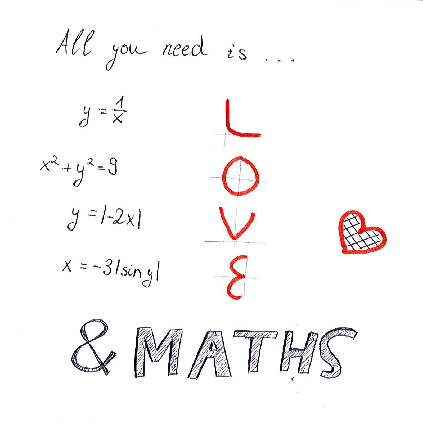
\includegraphics[width=7cm]{love_maths.png}
\end{center}
\end{framed}


\clearpage

\tableofcontents
%\pagenumbering{arabic}

\clearpage
\clearpage 

\section*{Abberviations}

\begin{tabular}{ll}
	LMI & linear matrix inequality 
	\\ LP & linear program or linear programming 
	\\ NLP & non-linear program or non-linear programming 
	\\ POP & polynomial optimization program or polynomial optimization
	\\ PSD & (symmetric) positive semidefinite
	\\ SDP & (linear) semidefinite optimization program or semidefinite programming
	\\ SOS & sum of squares
\end{tabular}

\clearpage 

\section*{About these notes} 

In July 2017, Prof.~Sebastian Sager and I held a course aiming at presenting some of the trends in modern optimization. This course is one of the teaching activities of the Research Training Network Mathematical Aspects of Complexity Reduction, supported by the German Research Foundation. Sebastian presented various aspects of linear, non-linear, mixed-integer and global optimization and also addressed optimization in infinite-dimensional spaces (in systems and control theory). 

In my part of the course, I explained the reduction of polynomial optimization problems to semidefinite optimization via the sum-of-squares approach, and explained how the interior point methods can be used to solve semidefinite problems based on the duality of semidefinite programming. This manuscript presents the notes, on which my part of the course was based.

Currently, there are several regular sources, from which you can learn about the topic: a long expository article of Monique Laurent~\cite{laurent2009sumsofsquares}, the book of Jean B.~Lasserre~\cite{lasserre2015anintroduction}, which is the standard reference book in polynomial optimization and the book of Murray Marshall~\cite{marshall2008positivepolynomials} that contains the necessary theoretical background from real algebra and ends with a short discussion of polynomial optimization.  There are basic dual approaches to reduce polynomial problems to semidefinite programming: one can use sum-of-squares relaxations and truncated-moment relaxations. In my notes, I discuss truncated-moment relaxations very briefly and towards the end of the notes. The line of thought is as follows: 
\begin{enumerate}
	\item To obtain lower bounds we need algebraic certificates for positivity; Sums of squares of polynomials turn out to be a very nice tractable certificate that can be expressed in terms of semidefinite optimization. Unfortunately, one cannot use sums of squares of polynomials to always certify positivity.
	\item One can always use sums of squares of rational functions, which shows that positivity is intrinsically related to sums of squares.
	\item On compact semialgebraic sets, positivity \emph{can} be expressed through sums of squares of polynomials. 
	\item For solving semidefinite problems, one needs to understand duality of semidefinite programming, which is a special case of conic duality. 
	\item Semidefinite programs can be solved using interior point methods. 
\end{enumerate}

Each of the above points corresponds to a chapter of these notes. Discussing point~3 I rely on my short exposition article \cite{averkov2013constructive} on elementary approaches to denominator-free positivstellensätze, which collects various pieces of information that were spread all over the literature. 

I made no attempt to give an extensive exposition of the background literature (though I plan to extend the literature list in the future).

A second iteration of the compact course based on these notes was held by Maximilian Merkert in 2020, whom I would like to thank for implementing some corrections compared to the initial version.

If you happen to spot any issues (inconsistencies etc.), please let me know. 

\clearpage 

\section{Introduction}



\subsection{Global non-linear optimization} 

\begin{itemize}
	%
	\item Convex and linear optimization problems are computationally tractable. This is confirmed in theory and practice! One very special thing about convex optimization is that there is no difference between local and global optimality. So, for checking global optimality, local information is enough.
	%
	\item In applications, one frequently needs to solve non-linear problems. When one says \emph{non-linear} one usually means \emph{non-convex problems}, because in optimization the crucial difference is not between linear and non-linear but between convex and non-convex.
	%
	\item Originally, one is usually interested in \emph{global non-linear optimization}. Of course, when the underlying global optimization problem is hard, one can try to find a locally optimal solution rather than solving the problem globally. However, if there are lots of local solutions of all possible qualities, why should a `random' local solution be good?  See figure: if you pick any locally optimal solution, you will get as good as any value of the objective function. So, why is a locally optimal solution any better than just any solution?
	\begin{center}
		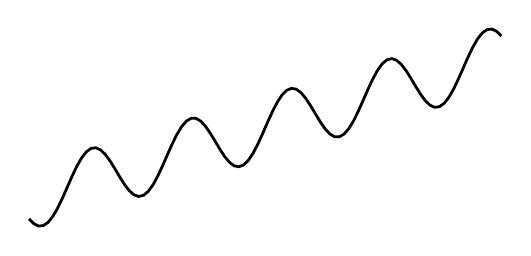
\begin{tikzpicture}
			\draw[line width=1pt,domain=-3:3,samples=100] plot ({\x}, {0.3*\x+0.4*sin(5*deg(\x))}); 
		\end{tikzpicture}
	\end{center}
%	\begin{center}
%		\begin{tikzpicture}
%		\begin{axis}[domain=0:3,legend pos=outer north east,,samples=100]
%		\addplot {0.3*x+0.2*sin(10*deg(x))}; 
%		%\legend{$x+ 6 \sin(x)$}
%		\end{axis}
%		\end{tikzpicture}
%	\end{center}
	%
	\item So, if we are really interested in solving an original problem, we usually have to deal with global non-linear programming (NLP).
	%
	\item \emph{General} global NLP is extremely hard. It's a \emph{huge} class of problems. Depending on how you define it, not algorithmically solvable. Consider the feasibility problem 
	\begin{align*}
		\sin(\pi x_1) = \ldots = \sin(\pi x_n) & = 0 & & \text{(Integrality constraints $x_1,\ldots,x_n \in \Z$)}
		\\ p(x_1,\ldots,x_n) & = 0 & & \text{(Polynomial equality)}
	\end{align*}
	It is not algorithmically solvable (see Matyasievich's answer to Hilbert's 10th problem). If you do not like the feasibility formulation you can reword the problem equivalently as an optimization problem. Just ask whether the optimal value of the minimization problem
	\[
		\inf \setcond{p(x_1,\ldots,x_n)^2 + \sum_{i=1}^n \sin(\pi x_i)^2}{x=(x_1,\ldots,x_n) \in \R^n} 
	\]
	is $0$ and if this value is attained for some $x \in \R^n$.
	
	%
	\item Take a look at the \blue{following chain of complexity classes}
	\[
		\complP \subseteq \complNP \subseteq \complPSPACE \subseteq \complEXP \subseteq \complDECIDABLE
	\]
	It is conjectured that all inclusions are strict and the inclusion $\complP \subseteq \complEXP$ is known to be strict. As we have seen, global NLP is not decidable and so it is easy to imagine that subclasses of global NLP are spread all over this chain. So, \blue{they cover} lots of extremely difficult problems, including the $\complNP$-complete problems, which researchers have already been working \blue{on} for decades. 
	
	Complexity theory tells us that there is no way of finding a \emph{universal} efficient approach to very hard problems. Still, we can and will develop some quite general theory which can help us to do appropriate algorithmic choices for our concrete problems we want to solve. 
	%
	\item Currently, the global NLP community seems to be split into two sub-communi\-ties:
    \begin{itemize}
	 \item One can use
  	 \begin{itemize}
		\item branching,
		\item introducing intermediate variables to keep track of the intermediate results in the expression digraphs of the underlying functions, or
		\item basic outer convexification (McCormick, $\alpha$-relaxations  et al.)
	\end{itemize}
	Such techniques are available in solvers like Baron. 

    \item Alternatively, one can use sums-of-squares which has also been implemented.
    \end{itemize}
\end{itemize}
	
\subsection{Polynomial optimization}

I what follows, I am going to use POP to abbreviate either \emph{polynomial optimization} or a \emph{polynomial optimization problem}. 

POP is the class of problems of dealing with optimization of
\begin{itemize}
	\item a polynomial objective function 
	\item in the presence of finitely many real-valued decision variables and 
	\item under finitely many polynomial equality/inequality constraints
\end{itemize}

Direct usage of equality constraints can be avoided, as we can replace $p(x)=0$ by $p(x) \ge 0$ and \blue{$-p(x) \ge 0$}. When we talk about inequality constraints, we mean the non-strict inequalities by default, but it can easily be seen that strict inequalities can be easily modelled via non-strict ones in lifting in the context of POP. Indeed $p(x) >0$ can be expressed as $p(x) y = 1$ and $y \ge 0$ using an additional variable $y$. 

We'll see how POPs can be converted to so-called semidefinite problems (SDPs). Some more specific situations can also be converted to linear problems (LPs). For LPs and SDPs various efficient solution methods can be employed. 

General POP involves a lot of kinds of problems as special cases, including the following $\complNP$-hard) problems:
\begin{itemize}
	\item Binary integer linear programming (so there is a connection to \emph{combinatorial optimization})
	\item Inequality constrained quadratic programming (and so there is a connection to classical numerical \emph{nonlinear optimization} dealing with iterative methods based on first and second derivatives and Taylor expansions). 
\end{itemize}

Since on a compact set, every continuous function can be approximated by a polynomial (Stone-Weierstrass theorem) with any given accuracy, in some sense, POP is dense in NLP. Apart from that, polynomials provide a very natural `modeling language', because arithmetics over reals (multiplication and addition) is one of the basic things a computer can do.  

There exist results showing that the decision version of polynomial optimization is in $\complEXP$ (see \cite{MR3212780}), so polynomial optimization (in its decision form) is somewhere between $\complNP$-hard and $\complEXP$ (but I do not know its precise complexity). 

%In my part of the lectures I would like to present algebraic approaches to \emph{global} nonlinear programming. We consider the family POP of polynomial optimization problems which is a very interesting subset of NLP. One can define POP as problems of optimizing a polynomial function on $\R^n$ subject to a finite system of non-strict polynomial inequalities (equalities can be easily modeled through inequalities). In some sense, POP is almost equal to NLP (kind of dense subset). Sebastian Sager has already presented the main approaches of the `non-linear optimization community' to NLP. 

%From the mathematical viewpoint, POP is interesting because of its relations to algebra,a and the hope is that algebraic theory may help for POP. Many concrete examples of NLP problems are actually POP problems. 

%In last decades, beautiful solutions techniques for POP have been developed which based on reduction of POP to convex problems through the so-called semidefinite optimization. POPs can be reduced to a hierarchy of large-size semidefinite problems (SDPs). This reduction is based on a certain duality theory for POP (Positivstellensätze). One can solve SDPs using interior-point methods for conic programming. Note that SDP is a far-reaching generalization of LP (One has LP $\subseteq$ SOP $\subseteq$ SDP, where SOP is a second-order cone programming, and all the paradigms are interesting in their own right). There exist interior-point methods tailored to conic problems, most notably to SDPs.

\subsection{Prerequisites}

The more you know about the following topics, the easier it would be for you to follow the discussion. 

\begin{itemize}
	\item[] \emph{Linear algebra}. Vector spaces, Euclidean spaces, linear maps. 
	\item[] \emph{Convexity}. Convex sets and cones, polyhedra, separations theorems, faces and extreme points. In the standard mathematics curriculum, convexity is usually integrated into introductory optimization courses.
	\item[] \emph{Linear optimization}. Duality, understanding the geometry of the simplex method. 
	\item[] \emph{Analysis}. Basic knowledge. 
	\item[] \emph{Algebra}. A bit of experience with groups, rings (and ideals), and fields. 
\end{itemize}

\subsection{Notation} 

\begin{tabular}{lll}
Set relations:	& & 
\\		& $\subseteq$ & regular inclusion 
\\ 		& $\varsubsetneq$ & proper inclusion
\\ Sets of numbers: & &
\\ & $\N$  & positive integers (called natural numbers here)
\\ & $\Z_+$ & non-negative integers
\\ & $\Q$ & rational numbers
\\ & $\R$ & real numbers
\\ & $\compl$ & complex numbers
\\ & $\R_+$ & non-negative reals 
\\ & $\R_{\ge 0}$ & non-negative reals (another notation)
\\ & $\R_{>0}$ & positive reals
\\ & $[m]$ & natural numbers not greater than $m \in \Z_+$
\\ Operations for sets: & & 
\\ & $\intr$ & interior
\\ &  $\conv$ & convex hull
\\ &  $\cone$ & \emph{convex} conic hull
\\ & $\lin$ & linear hull
\\ & $\aff$ & affine hull
\end{tabular} 

We use $0$ to denote the zero element; it can be zero value, zero vector or a zero matrix, depending on the context. 

Throughout, $n \in \N$ is the dimension of the ambient space, which is usually $\R^n$. The elements of $\R^n$ are viewed as columns, but we tend to omit transposition to simplify the expressions. For example, we write $(1,2,3) \in \R^3$ rather than $(1,2,3)^\top \in \R^3$. If $I$ is a set, then $\R^I$ is the set of all functions from $I$ to $\R$ and it can also be viewed (and written) as a vector indexed by elements of $I$. So, we can write for example $x=(x_i)_{i \in I} \in \R^I$. With this point of view, $\R^n$ is nothing but a special case of $\R^I$ with $I=[n]$. Please note that we do not insist $x_i$ to be the default notation for the $i$-component, because in cases we do not work with components of vectors, we prefer to use lower indexing for vectors. 

For $x= (x_i)_{i \in [n]}$ and $y = (y_i)_{i \in [n]}$, we introduce the standard scalar product $\sprod{x}{y} = \sum_{i=1}^n x_i y_i$ of $x$ and $y$ and the respective Euclidean norm $\|x\| := \sqrt{\sprod{x}{x}}$ of $x$. We also use the notation $\sprod{\dotvar}{\dotvar}$ and $\|\dotvar\|$ to denote the scalar product and the respective norm of other Euclidean spaces appearing in our discussion. The scalar product gives rise to the orthogonality relation and we use the notation $X^\perp$ to denote the orthogonal complement of $X$ (which is the set of all vectors orthogonal to every vector from $X$). 

By $I_n$ we denote the identity matrix of size $n$, and if the size is clear from the context we omit the subscript $n$. If $A$ is a matrix, then $A^\top$ denotes the transpose of~$A$. When we say that a matrix $A$ is PSD we always mean symmetric PSD.



Asymptotic notation for $f, g: X \to \R$, for $x \to x^\ast$:

\begin{center}
\begin{tabular}{l@{\hskip 5em}l}
	$f=O(g)$ & $\limsup_{x \to x^\ast} \frac{|f(x)|}{|g(x)|} < +\infty$ 
	\\ $f=\Omega(g)$ & $\liminf_{x \to x^\ast} \frac{|f(x)|}{|g(x)|} < +\infty$ 
	\\ $f = \Theta(g)$ & $f= O(g)$ and $f = \Omega(g)$
	\\ $f = o(g)$ & $\lim_{x \to x^\ast} \frac{|f(x)|}{|g(x)|} = 0$. 
\end{tabular}
\end{center}


By $\R[X_1,\ldots,X_n]$ we denote the set of polynomials in variables $X_1,\ldots,X_n$ with coefficients in $\R$. Instead of $\R$ one can use other sets, so one can consider other sets of polynomials, but we'll mostly work with $\R[X_1,\ldots,X_n]$. A warning for those, who don't have much experience with algebra: polynomials and functions are not quite the same thing. Rather, polynomials are formal expressions, and their variables $X_1,\ldots,X_n$ are just formal symbols (also called \emph{indeterminates}). So, a symbolic variable $X$ in the ring $\R[X]$ of univariate polynomials with real coefficients is not equal to any element of $\R$, because $X$ is just another element of $\R[X]$ (as any element of $\R$). To illustrate this, consider the following code in sage which introduces a symbol variable and compares it to the number $3$: 

\begin{verbatim}
x = var('x')
if x!=3:
   print "Not equal"
else:
   print "Equal"
\end{verbatim}

You can try this code at \url{http://sagecell.sagemath.org/}. Another way to explain this is by means of coefficients. The element $3$ of $\R[X]$ is a degree one polynomial, that is $3 = 3 + 0 X + 0 X^2 + \ldots $, and its coefficients are $3, 0, 0, \ldots$. On the other hand $X$ is another polynomial $X = 0  + 1 X + 0 X^2 + \cdots$ and its coefficients are $0, 1,0 , 0, \ldots$. Comparison of polynomials is defined through comparision of coefficients and so $3$ and $X$ are not equal, because their respective coefficients are not all equal. 

$\R(X_1,\ldots,X_n)$ denotes the set of rational functions in $X_1,\ldots,X_n$ with coefficients in $\R$. Even though rational functions are called functions, they are not functions but formal quotients $f/g$ with $f, g \in \R[X_1,\ldots,X_n]$ and $g \ne 0$. By definition, two such functions $f_1/ g_1$ and $f_2/g_2$ are equal if the polynomial equality $f_1 g_2 = f_2 g_1$ holds. 

For various kinds of structures \blue{$X$ and $Y$,} we use notations like $X + Y = \setcond{ x + y}{x \in X, y \in Y}$, $X - Y = \setcond{x - y}{x \in X, y \in Y}$, $a X = \setcond{ a x }{x \in X}$ etc. This allows us to express things in a concise form. For example, if $R$ is a ring, then an ideal $I$ of $R$ can be defined as an additive subgroup of $R$ satisfying $R I \subseteq I$, where we use the notation $X Y = \setcond{x y }{x \in  X, y \in Y}$. 


\subsection{Numbering}

Theorems, Lemmas, Propositions, Remarks, Exercises and Examples are all numbered based on a common counter. In my opinion, this simplifies searching. 

\subsection{Software}

The following software will or may be useful:

\begin{center}
\begin{tabular}{lp{9.7cm}c}
	\textbf{Name} & \textbf{Description} & \textbf{Used}
	\\ \hline MATLAB & proprietary numerical computing environment & yes
	\\ GNU Octave & free alternative for MATLAB & no
	\\ \hline AMPL & modelling language for optimization problems & yes
	\\ \hline SeDuMi & MATLAB package for solving semidefinite problems & yes
	\\ \hline SOSTOOLS & sums-of-squares based optimization toolbox for MATLAB & yes
	\\ GloptyPoly & sums-of-squares and moment-relaxation based optimization toolbox for MATLAB & no
	\\ \hline BARON software &  global solver for non-convex problems & yes
\end{tabular}
\end{center}

One could have listed more software.



\clearpage 
\section{Non-negativity and sums of squares} 

In this chapter, $n \in \N$ and  
\[
X=(X_1,\ldots,X_n)
\]
is a tuple of $n$ indeterminates. In particular, if $n=1$, then $X$ is an indeterminate. The aim is to present the relationship between real algebra, polynomial optimization and semidefinite optimization. 

\subsection{A Topic of real algebra}

In contrast to classical algebra over complex numbers (or more generally, over algebraically closed fields), in real algebra one tries to understand positivity and non-negativity of polynomials and other algebraic objects (one just cannot define the non-negativity concept over complex numbers). So, we have to work with reals (or ordered fields, more generally). 

Let $f \in \R[X]=\R[X_1,\ldots,X_n]$. For $K \subseteq \R^n$, we write 
\begin{itemize}
	\item $f \ge 0$ on $K$ if $f(x) \ge 0$ for every $x \in K$ and 
	\item $f > 0$ on $K$ if $f(x)> 0$ for every $x \in K$.
\end{itemize}

%\begin{exercise}
%	If $f \in \R[X] \setminus \{0\}$ is non-negative on $\R^n$, then the degree of $f$ is even. 
%\end{exercise}
%\begin{solution}
%	Assume the contrary, and the degree $d$ is odd. We consider all exponents $X^\alpha$ of odd degree $d$ occuring in $f$. The exponent vector $\alpha = (\alpha_1,\ldots,\alpha_d)$. 
%\end{solution}

We'll frequently write polynomials $f \in \R[X]$ using coefficients $c_\alpha \in \R$ where $\alpha \in \Z_+^n$. For monomials we use the notation
\[
	X^\alpha := X_1^{\alpha_1} \cdots X_n^{\alpha_n}  \qquad (\alpha \in \Z_+^n),
\]
so that we can write $f$ in the form 
\[
	f = \sum_{\alpha \in \Z_+^n} c_\alpha X^\alpha
\] 
where all but finitely many $c_\alpha$'s \blue{are zero}. 
We call $\alpha \in \Z_+^n$ an \emph{exponent vector} or a \emph{multi-index} and we use the notation
\[
	|\alpha| := \alpha_1 + \cdots + \alpha_n
\]
to denote the degree of the monomial $X^\alpha$. For $n \in \N$ and $d \in \Z_+$, we introduce the notation 
\[
	E^n_d := \setcond{\alpha \in \Z_+^n}{|\alpha| \le d}
\]
for \blue{the set of} multi-indices of degree at most $d$. Thus, if $\deg(f) \le d$, we can write $f$ as $f = \sum_{\alpha \in E^n_d} c_\alpha X^\alpha$. 

\begin{exercise}
	Determine the cardinality $|E^n_d|$ of $E^n_d$.
\end{exercise}
\begin{solution}
	We are looking for the number of \blue{ordered} non-negative integer solutions of the inequality $\alpha_1 + \cdots + \alpha_n \le d$.  Adding $\alpha_{n+1} \in \Z_+$ we switch to looking for the number of non-negative integer solutions of the equality  $\alpha_1 + \cdots + \alpha_{n+1} = d$ in unknowns $\alpha_1,\ldots,\alpha_{n+1}$. 
		
	Substituting, $\alpha_i + 1 =: \beta_i$, we switch to looking for the number of positive integer solutions of the equation $\beta_1 + \cdots + \beta_{n+1} = d+n+1$. Now imagine you've got $d+n+1$ objects, which are lined up, like in this example with $d+n+1 = 8$ objects
	\[
		\square \ \square \ \square \ \square \ \square \ \square \ \square \  \square 
	\]
	Now, there are $d+n$ spaces between the objects and by marking $n$ of the spaces as the separating spaces you can split your objects into $n+1$ non-empty groups of consecutive objects. If say, $n=3$ the following marks
	\[
	\square \ \square \cdot \square \ \square \cdot \square \cdot \square \ \square \  \square 
	\]
	split the objects in four groups with, respectively, $2$, $2$, $1$ and $3$ objects. So, each such splitting corresponds to a unique choice of $\beta_1,\ldots,\beta_{n+1}$ and, vice versa, each choice of $\beta_1,\ldots,\beta_{n+1}$ gives a unique splitting. In our example, we get \blue{$\beta_1 = 2, \beta_2 =2,\beta_3=1, \beta_4=3$}. The number of splittings is clearly $\binom{n+d}{n}$ since we choose $n$ spaces out of $n+d$. This shows $|E_d^n| = \binom{n+d}{n}$ and since the binomial coefficients are symmetric we also have $|E_d^n|  = \binom{n+d}{(n+d)-n} = \binom{n+d}{d}$. 
\end{solution}

\subsection{Unconstrained polynomial optimization}

For the time being, let's restrict our attention to unconstrained polynomial optimization. It is a sufficiently large class, on the one hand, and it is a convenient class to explain the basic ideas of approaching POP via SOS, on the other hand. 

We are given a polynomial objective $f \in \R[X]$ and want to solve 

\begin{equation}
	\inf \setcond{f(x)}{x \in \R^n}. \label{unconst:POP:eq}
\end{equation}

Solving the problem means, as usual, to determine the optimal value which can be finite, $-\infty$ or $+\infty$ and, if there exists an $x^\ast \in \R^n$, at which the optimal value is attained, one such $x^\ast$ should be computed. Currently, we do not go into the subtleties on what it actually means to compute $x^\ast$. So, the statement of the problem is a bit vague, but that's not really disturbing, because we are not going to do computational-complexity studies so far. 


\begin{exercise}
	Show that for $n=1$, whenever the infimum in \eqref{unconst:POP:eq} is finite, it is attained at some $x \in \R^n$ and that for every $n \ge 2$, there exists a polynomial $f$ such that the optimal value of \eqref{unconst:POP:eq} is finite but not attained at any $x \in \R^n$. 
\end{exercise}
\begin{solution}
	As for $n=1$, we see that for $|x| \to \infty$, the dominating term will be the one for the monomial of the highest degree. The degree must be even, say $2d$, for otherwise, the polynomial wouldn't be bounded from below. The coefficient at $2d$ should be positive by the same reasons. So we see that $f(x)>0$ if $x$ is sufficiently large. Thus, \eqref{unconst:POP:eq} can be turned into the optimization of a polynomial over a \blue{closed} segment. Since polynomial functions are continuous, we are done. 
	
	As for $n \ge 2$, of course it is sufficient to deal with the case $n=2$. Consider $f(X_1,X_2) := X_2^2 + (X_1 X_2 -1)^2$. The infimum is zero, because $f$ is nonnegative on $\R^2$ and $\blue{f(1/t,t)} = t^2 \to 0$ as $t \to 0$. Let $x_1, x_2 \in \R$. If $x_2 \ne 0$, then $f(x_1,x_2) \ge x_2^2 > 0$. If $x_2=0$, then $f(x_1,x_2) \ge 1 > 0$. 
\end{solution}

\subsection{Sum-of-squares relaxation from the dual formulation}

Approaches to solving \eqref{unconst:POP:eq} (and other polynomial problems) can be roughly split into heuristic and non-heuristic ones. For the former, a choice of $x^\ast \in \R^n$ is suggested, but one does not say whether the chosen $x$ is good (no guarantees). For the latter, one does suggest $x^\ast$ and gives a lower bound $y$ on the optimal value, so that by comparing $f(x^\ast)$ and $y$ one can see how good $x^\ast$ actually is. Heuristic approaches to solving general problems is a very popular topic (machine learning and neural networks etc.) In this course, we are interested in non-heuristic approaches. So, anyway we need an approach to derive lower bounds, and that's what we're actually going to start with. Let's formally dualize our problem \eqref{unconst:POP:eq} to

\begin{equation}
	\sup \setcond{y \in \R}{ f - y \ge 0 \quad \text{on} \ \R^n}. \label{unconst:POP:dual:eq}
\end{equation}

This formulation just tells us that we are interested in lower bounds (that's why `formally dualize'), because the formulation does not yet tell us how to actually find such bounds. While a non-negativity condition for a polynomial is hard to check, there is a stronger condition that turns out to be easy to test. We call $g \in \R[X]$ sum of squares (SOS), if $g= g_1^2 + \cdots + g_k^2$ for finitely many polynomials $g_1,\ldots,g_k \in \R[X]$. If we succeeded to write $g$ as above, we had an algebraic evidence of $g$ being non-negative. So, by strengthening the non-negativity constraint in \eqref{unconst:POP:dual:eq} by an SOS constraint, our supremum becomes smaller (in general) and we arrive at what is called an SOS relaxation of \eqref{unconst:POP:eq}. 

\begin{equation}
\sup \setcond{y \in \R}{ f - y \quad \text{SOS}}. \label{unconst:POP:dual:SOS:eq}
\end{equation}

The term relaxation should be understood in the sense that by solving \eqref{unconst:POP:dual:SOS:eq} we obtain a \emph{lower} bound on our original problem \eqref{unconst:POP:eq}. 

In what follows we've got two things to take care of: we need to figure out how we could solve  \eqref{unconst:POP:dual:SOS:eq}, and it would be good to understand how good the lower bounds on \eqref{unconst:POP:eq} obtained from \eqref{unconst:POP:dual:SOS:eq} are.


\subsection{SOS-relaxations and semidefinite optimization}

\label{SOS:and:sdp}

For $k \in \N$, let $\cS^k$ be the vector space of symmetric matrices $A \in \R^{k \times k}$ of size $k \times k$ and let $\cS_+^k$ be the closed convex cone of psd matrices in this space. The constraint `$Z \in \cS_+^k$' can be viewed as a generalization of non-negativity to the world of matrices. For $k=1$, we just have a regular non-negativity constraint for \blue{a real variable}.

A \emph{(linear) semidefinite problem} (SDP, for short) is a problem with the following properties:
\begin{itemize}
	\item Linear objective
	\item Finitely many variables, which can be real variables ranging in $\R$ or matrix variables in spaces $\cS^k$ with $k \in \N$
	\item Finitely many constraints of the form
	\[
		A_0 + x_1 A_1 + \cdots + x_n A_n \in \cS_+^k,
	\]
	with $A_0,\ldots,A_n \in \cS^k$. The latter is called a \emph{linear matrix inequality} (LMI) of size $k$ for real variables $x_1,\ldots,x_n \in \R$. The matrices $A_0,\ldots,A_n$ are the coefficients of the LMI. (Note that if $A_0,\ldots,A_n$ are diagonal matrices, we just have a system of $k$ linear inequalities). 
	\item Constraints of the form
	\[
		Z \in \cS_+^k
	\]
	with $k \in \N$. The latter is called a PSD-constraint on a matrix-variable $Z$. 
	\item Linear equality constraints involving the real variables and/or entries of the matrix variables.
\end{itemize}

We'll see that \eqref{unconst:POP:dual:SOS:eq} can be formulated as a semidefinite problem. It is enough to derive the following 

\begin{proposition}
	\label{sos:as:sdp:feasibility}
	Let $d \in \Z_+$. Let $f = \sum_{ \gamma \in E_{2d}^n} c_\gamma X^\gamma \in \R[X]$ be a polynomial of degree at most $2d$. Then the following conditions are equivalent:
	\begin{enumerate}[(i)]
		\item The polynomial $f$ is SOS. 
		\item There exists a symmetric psd matrix $Z:= \bigl(z_{\alpha,\beta})_{\alpha,\beta \in E_d^n}$ satisfying the linear \blue{equations}  
		\begin{equation}
			\sum_{\alpha, \beta \in E_d^n \, : \, \alpha + \beta = \gamma} z_{\alpha, \beta} = c_\gamma \qquad \forall \ \gamma \in E_{2 d}^n \label{SOS:sdp:eq}
		\end{equation}
	\end{enumerate}
\end{proposition}
\begin{proof}
	We introduce the vector of all monomials of degree at most $d$: 
	\[
		m(X):=(X^\alpha)_{\alpha \in E_d^n}.
	\]
	
	If $f = f_1^2 + \cdots + f_r^2$ for some $f_1,\ldots,f_r \in \R[X]$, then all $f_1,\ldots,f_r$ are of degree at most $d$ (this will be justified below, in Proposition~\ref{newton:SOS}). For each $f_j$ we introduce the vector $u_j \in \R^{E_d^n}$ of its coefficients, so that we can write $f_j$ as 
	\[
		f_j = \sprod{m(X)}{u_j} = m(X)^\top u_j = u_j^\top m(X).
	\]
	Thus, $f_j^2 = \sprod{m(X)}{u_j}^2 = m(X)^\top u_j u_j^\top m(X)$ and $f=f_1^2 + \cdots + f_r^2$ can be rewritten as 
	\[ 
		\blue{f = m(X)^\top \underbrace{(u_1 u_1^\top + \cdots + u_r u_r^\top )}_{=:Z} m(X).}
	\]
	For each $j$, the matrix $u_j u_j^\top$ is psd (of rank at most $1$). Hence, the sum $Z = (z_{\alpha,\beta})_{\alpha,\beta \in E_d^n}$ is psd, too. We arrive at the representation 
	\[
		\blue{f} = m(X)^\top Z m(X).
	\]
	The latter can be described as a system of linear \blue{equations in}  the coefficients of~$Z$, \blue{and this system is written explicitly as \eqref{SOS:sdp:eq}.} 
	
	Conversely, if \eqref{SOS:sdp:eq} is fulfilled, then we have $\blue{f}= m(X)^\top Z m(X)$. Since $Z$ is psd, we can write it as $Z = \sum_{j=1}^r u_j u_j^\top$ for some finitely many vectors $u_1,\ldots,u_r \in \R^{E_d^n}$. This yields \blue{$f=f_1^2 + \cdots + f_j^2$} for $f_j = \sprod{m(X)}{u_j}$. 
\end{proof}

In the last step of the previous proof, we used a fact from linear algebra, which we formulate as an exercise

\begin{exercise}
	\label{sdp:sum:rank:1}
	Show that if a matrix $A \in \cS^k$ is psd, then it can be written as $A = u_1 u_1^\top + \cdots + u_r u_r^\top$ for some finitely many vectors $u_1,\ldots,u_r \in \R^k$. Can the choice of $r$ be bounded in terms of $k$?
\end{exercise}
\begin{solution}
	We use $r=k$. 
	
	\emph{Showing existence:} This solution is based on the spectral theory of symmetric matrices. 
	Since $A$ is symmetric, there exists an orthonormal basis $v_1,\ldots,v_k$ consisting of eigenvectors of $A$. Let $\lambda_1,\ldots,\lambda_k$ be the respective eigenvalues. Since $A$ is psd, the eigenvalues are non-negative. Let $u_j = \sqrt{\lambda_j} v_j$. It suffices to check that $A v_j = (u_1 u_1^\top + \cdots + u_k u_k^\top) v_j$ for every $j\in[k]$. The left as well as the right hand side is $\lambda_j v_j$. Clearly, if $A$ is of rank $k$, we cannot choose a smaller $r$, since the rank of $u_1 u_1^\top + \cdots + u_r u_r^\top$ is at most $r$. 
	
	\emph{Computing the decomposition:} There is a Gauss-method-like approach to diagonalizing a given quadratic form with $O(k^3)$ arithmetic operations. This would definitely do. 
	
	Every psd matrix $A$ has a Cholesky factorization $A = L L^\top$, where $L$ is a lower triangular matrix. For us, it is not of primary importance that $L$ is lower triangular (any matrix $L$ with $A = LL^\top$ would do). 
	Choosing $u_1,\ldots,u_k$ to be the columns of $L$ we get a desired representation of $A$. Note that, on the algorithmic side (when one really wants to find a decomposition $A=L L^\top$ efficiently), one usually presents how to efficiently compute a Cholesky decomposition of positive definite matrices. For positive semidefinite matrices, the existence of such a decomposition can be shown as follows. 
	
	
	Every decomposition $A=UU^\top$, where $U$ is arbitrary, gives a decomposition $A=LL^\top$, because $U^\top$ has a QR-factorization. 
	
	On the level of software, I've tried out the function \textbf{chol} in Matlab but it does not seem to accept matrices of non-full rank (there has been a respective error message). What one can do to compute a desired decomposition within a few lines of code is taking a square root of the matrix using \textbf{sqrtm}. Here is the code illustrating the two possibilities:
	
	\lstinputlisting[language=Matlab]{code/chol_example.m}	
	
	The code generates a random positive semidefinite matrix and uses the two approaches to get the decomposition. So, both $R^\top R$ and $V^\top V$ coincide with $A$ (in the numerical sense). 
\end{solution}

With Proposition~\ref{sos:as:sdp:feasibility} we can easily convert the SOS-relaxation to an SDP. 

\begin{corollary}
	Let $f \in \R[X]$ be of degree at most $2 d$, where $d \in \Z_+$. Then \eqref{unconst:POP:dual:SOS:eq} is an SDP of the form
	\begin{equation}
		\sup \setcond{y \in \R}{Z \ \textpsd, \  m(X)^\top Z m(X) + y = \blue{f}}. \label{unconst:POP:dual:SOS:as:sdp:eq}
	\end{equation}
	where $m(X) := (X^\alpha)_{\alpha \in E^n_d}$ and the decision-variable $Z$ is a $k \times k$ symmetric matrix with $k=|E^n_d|$. 
\end{corollary}

The linear equality system 
\[
	m(X)^\top Z m(X) + y = \blue{f}
\]
in unknowns $Z$ and $y$ can be written explicitly, similarly to the system \eqref{SOS:sdp:eq}, but one can use also the above concise form. Already from this form it is clear that this is a linear system: $\blue{f}$ is the right hand side of the system and $Z$ and $y$ occur linearly in the left hand side.

The total number of variables of the latter system is \blue{$\binom{k+1}{2}+1 \in O(k^2)$}, where $k = \binom{n+d}{d}$ and the number of equations is $|E_{2d}^n| = \binom{n+2d}{2d}$. 

\subsection{Employing Newton polytopes to reduce the size of an SDP} 

It turns out that, by taking more care to what our choice of $f$ actually is, the size of \eqref{unconst:POP:dual:SOS:as:sdp:eq} can be reduced. For a polynomial $f = \sum_\alpha c_\alpha X^\alpha \in \R[X]$ the set 
\[
	\newt(f) := \conv \setcond{ \alpha }{c_\alpha \ne 0}
\]
is called the \emph{Newton polytope} of $f$. We want to find out how the Newton polytope of a sum of squares looks like.  

\begin{lemma}
	\label{Newton:of:square}
	For every $f \in \R[X]$ one has $\newt(f^2) = 2 \newt(f)$. 
\end{lemma}
\begin{proof}
	We assume $f \ne 0$. If $f = \sum_{\alpha \in E} c_\alpha X^\alpha$ with $c_\alpha \ne 0$ for all $\alpha \in E$, then $\newt(f) = \conv(E)$. We've got $f^2 = \sum_{\alpha, \beta \in E} c_\alpha c_\beta X^{\alpha + \beta}$. This shows that $\newt(f^2) \subseteq \conv(E+E) = \conv(E)+\conv(E) = 2 \newt(f)$. To see the converse let $\alpha$ be a vertex of $\newt(f)$. Then, for all $\beta,\gamma \in E$, whenever one has $\alpha = (\beta+ \gamma)/2$, one must have $\beta=\gamma=\alpha$. In other words, one can have $2 \alpha = \beta + \gamma$ for $\beta,\gamma \in E$ if and only if $\beta=\gamma=\alpha$. This shows that $X^{2\alpha}$ occurs in $f^2$ with coefficient $c_\alpha^2 \ne 0$. Thus, we also have the converse inclusion $2 \newt(f) \subseteq \newt(f^2)$. 
\end{proof}

The latter can be \blue{generalized} to

\begin{proposition} \label{newton:SOS}
	Let $f_1,\ldots,f_r \in \R[X]$ and let $f=f_1^2 + \cdots + f_r^2$. Then, we have
	\[
		\newt(f) = 2 \conv \left( \bigcup_{j=1}^r \newt(f_j) \right),
	\]
	and, in particular, 
	\[
		\deg(f) = 2 \max \{\deg(f_1),\ldots,\deg(f_r)\}. 
	\]
\end{proposition} 
\begin{proof}
	The argument is inspired by Proposition~1.1 of \cite{chua2016gram} (which is a somewhat weaker formulation of this proposition). It seems that the idea of looking at the Newton polytope for non-negativity questions goes back to Reznick \cite{Reznick1978} (I do not have access to this paper). 
	
	Without loss of generality let all $f_j$ be non-zero polynomials. The inclusion $\subseteq$ follows by observing $\newt(f_1^2 + \cdots + f_r^2) \subseteq \conv \left(\bigcup_{j=1}^r \newt(f_j^2) \right)$ and using Lemma~\ref{Newton:of:square}.
	
	To see the converse consider an arbitrary vertex $\alpha$ of $P:=\conv \left( \bigcup_{j=1}^r \newt(f_j) \right)$. Then, for every $\beta,\gamma \in P \cap \Z^n$, the condition $\alpha = \frac{1}{2}(\beta + \gamma)$ implies $\beta = \gamma = \alpha$.  In other words the condition $2 \alpha = \beta+ \gamma$ for $\beta, \gamma \in P \cap \Z^n$ implies $\beta=\gamma =\alpha$. Each $f_j$ can be written as $f_j = \sum_{\beta \in P \cap \Z^n} c_{j,\beta} X^\beta$. From the previous condition, we see that $X^{2 \alpha}$ occurs in $f_1^2 + \cdots + f_r^2$ with the coefficient $\sum_{j=1}^r c_{j,\alpha}^2$. Since $\alpha$ is a vertex of one of the polytopes $\newt(f_j)$, at least one square in the previous sum is non-zero. We thus conclude that $2 \alpha \in \newt(f_1^2 + \cdots +f_r^2)$. 
	
	The equality for the degrees is an obvious consequence of the equality for the Newton polytopes (the information about the degree is saved in the Newton polytope). 
\end{proof}

For \eqref{unconst:POP:dual:SOS:as:sdp:eq} to be feasible, we need to have \blue{$f - y$ is SOS} for at least one $y \in \R$.
\blue{Such $y \in \R$ exists if and only if $\bar y \in \R$ with $\bar y \neq 0$ and $f - \bar y$ is SOS exists.
With such a choice $\newt(f) = \conv(\newt(f - \bar y) \cup \{0\})$.} So, by \blue{Proposition~\ref{newton:SOS}},  for feasibility it is necessary that \blue{$\newt(f)$} is of the form $2 P$, where $P$ is a polytope with integer vertices (so called integer polytope), \blue{and that one of its vertices is~$0$}. \blue{Proposition~\ref{newton:SOS}} also shows that in that case, we can use $m(X)$ of the form $m(X) = (X^\alpha)_{\alpha \in P \cap \Z^n}$. So, rather than using \blue{exponent vectors} from the whole set $\blue{E^n_d}$, we can restrict ourselves to $P \cap \Z^n$ (a subset of $\blue{E^n_d}$), so that the size of the SDP \eqref{unconst:POP:dual:SOS:as:sdp:eq} gets reduced. 

\begin{exercise}
	Consider 
	\[
	f = 2 + X_1^2 + X_1^2 X_2^4 - 4 X_1 X_2 
	\]
	\begin{enumerate}[(a)]	
		\item Show that the two-variate polynomial is SOS. 
		\item Determine a vector $m(X)$ of monomials and a PSD matrix $Z$ with 
		\[
			f=m(X)^\top Z m(X). 
		\]
		\item Describe, for your choice of $m(X)$, all PSD matrices $Z$ satisfying 
		\[
		f=m(X)^\top Z m(X).
		\]
	\end{enumerate}
\end{exercise}
%\begin{solution}
%	We have seen a general strategy that allows to answer such kind of questions numerically (some sdp-solvers also work with exact arithmetics). In the software session you will see how to use software (SOStools, sedumi) for answering these kind of questions. Here is a different solution, in which the approach was to tackle this particular $f$. Let us look at the exponent vectors and the Newton polytope of our polynomial $f$: 
%	\begin{center}
%		\begin{tikzpicture}[scale=0.5]
%		\draw[black!30!white,line width=1pt] (0,0) grid (2,4);
%		\draw[line width=1.2pt] (0,0) -- (2,0) -- (2,4) -- cycle;
%		\fill (0,0) circle (0.15) (1,1) circle (0.1) (2,4) circle (0.15) (2,0) circle (0.15);
%		\end{tikzpicture}
%	\end{center}
%	The Newton polytope is a nice triangle. We'll the triangle even better, if we flip it along the $x_1$ axis to arrive at
%	\begin{center}
%		\begin{tikzpicture}[scale=0.5]
%		\draw[black!30!white,line width=1pt] (0,0) grid (2,4);
%		\draw[line width=1.2pt] (0,0) -- (2,0) -- (0,4) -- cycle;
%		\fill (0,0) circle (0.15) (1,1) circle (0.1) (0,4) circle (0.15) (2,0) circle (0.15);
%		\end{tikzpicture}
%	\end{center}
%	In fact, if our Newton polytope were like that, then the underlying polynomial  would be particularly simple with only one monomial depending on both $X_1$ and $X_2$. 
	
%	The algebraic operations corresponding to this flip is taking the polynomial 
%	\[
%	g := X_1^2 f(X_1^{-1},X_2) = 2 X_1^2 + 1 + X_2^4 - 4 X_1 X_2.
%	\]
%	Now we see that the `flipped polynomial' is SOS. Indeed, $2X_1^2 - 4 X_1 X_2 = 2 (X_1^2 - 2 X_1 X_2) = 2 ( (X_1 - X_2)^2 - X_2^2)$, which gives 
%	\[
%	g = 2 (X_1-X_2)^2 + 1 - 2 X_2^2 + X_2^4 = 2 (X_1 -X_2)^2 + (1 -X_2^2)^2.
%	\]
%	This shows that $g$ is SOS. To get an SOS-representation for $f$, we need to `flip back'. That is,
%	\[
%	f(X_1,X_2) = X_1^2 g(X_1^{-1},X_2) = 2 (1 - X_1 X_2)^2 + X_1^2 (1-X_2^2)^2. 
%	\]
	
%	Alternatively, for carrying out a derivation automatically using SDP, we can also take into account the Newton polytope. The Newton polytope of $f$ is twice the triangle with vertices $(0,0), (1,0), (1,2)$. Apart from the vertices, there is another integer point $(1,1)$ inside. Thus, it suffices to deal with the four monomials $1, X_1, X_1 X_2, X_1 X_2^2$. As a result our LMI constraint will involve a $4 \times 4$ matrix
%	\[
%	Z:=\bordermatrix{
%		& 1 & X_1 & X_1 X_2 & X_1 X_2^2 
%		\cr 1 & z_{1,1} & z_{1,2} & z_{1,3} & z_{1,4}
%		\cr X_1 & z_{1,2} & z_{2,2} & z_{2,3} & z_{2,4}
%		\cr X_1 X_2 & z_{1,3} & z_{2,3} & z_{3,3} & z_{3,4}
%		\cr X_1 X_2^2 & z_{1,4} & z_{2,4} & z_{3,4} & z_{4,4}
%	}
%	\]
%	There are $10$ unknowns here, but actually some entries get filled uniquely. For example, looking at the vertices of the Newton polytope, we see that $z_{1,1} = 2, z_{2,2} = 1$ and $z_{4,4} = 1$. So, only $7$ unknowns remain (for which we get constraints further from the equation $f(X) = m(X)^\top Z m(X)$). 
%\end{solution}
\begin{solution} 
	Parts of this exercise can be solved just by guessing an SOS decomposition of $f$, which is a valid approach to solve exercises and it is quite feasible here because the polynomial $f$ is not too complicated. Anyway, we want to follow up the systematic approach we've just developed and see how the theory works for a concrete example. 
	Look at the \blue{exponent vectors} and the Newton polytope: 
		\begin{center}
			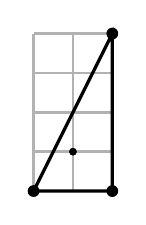
\begin{tikzpicture}[scale=0.5]
			\draw[black!30!white,line width=1pt] (0,0) grid (2,4);
			\draw[line width=1.2pt] (0,0) -- (2,0) -- (2,4) -- cycle;
			\fill (0,0) circle (0.15) (1,1) circle (0.1) (2,4) circle (0.15) (2,0) circle (0.15);
			\end{tikzpicture}
		\end{center}
		The necessary condition for SOS is fulfilled. It's twice a lattice polytope and the coefficient corresponding to the vertices are positive. Consider the half of the Newton polytope: 
		\begin{center}
			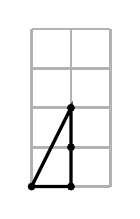
\begin{tikzpicture}[scale=0.5]
			\draw[black!30!white,line width=1pt] (0,0) grid (2,4);
			\draw[line width=1.2pt] (0,0) -- (1,0) -- (1,2) -- cycle;
			\fill (0,0) circle (0.1) (1,0) circle (0.1) (1,1) circle (0.1) (1,2) circle (0.1);
			\end{tikzpicture}
		\end{center}
		So, we know that we can choose $m(X)$ consisting of monomials with the vector exponents $00,10,11,12$. So, we'll need to come up with a matrix $Z$ whose rows and columns are indexed by $00,10,11,12$, and there will be linear equalities for the entries of $Z$ derived from the condition $f=m(X)^\top Z m(X)$. Let's see what results we obtain when we add two vectors from the list $00,10,11,12$: 
		\begin{align*}
			(0,0) & = (0,0) + (0,0)
			\\ (1,0) & = (0,0) + (1,0)
			\\ (1,1) & = (0,0) + (1,1)
			\\ (1,2) & = (0,0) + (1,2)
			\\ (2,0) & = (1,0) + (1,0)
			\\ (2,1) & = (1,0) + (1,1)
			\\ (2,2) & = (1,1) + (1,1) = (1,0) + (1,2)
			\\ (2,3) & = (1,1) + (1,2)
			\\ (2,4) & = (1,2) + (1,2)
		\end{align*}
		(the above equalities can also be nicely illustrated in a picture showing  $c= \frac{1}{2} (a+b)$ with $a,b$ being even integer vectors).
		So, we see that almost all entries of $Z$ are actually determined uniquely by $f$. The only entries, where we cannot guarantee uniqueness are $z_{11,11}$ and $z_{10,12}$. So, we will denote $z_{10,12}$ by $-t$ and then we see that one needs to have $z_{11,11}= 2t $, because of the relation $z_{11,11} + 2 z_{10,12} = 0$. 
		\[
		Z:=\bordermatrix{
			& 00 & 10 & 11 & 12
			\cr 00 & 2 & 0 & -2 & 0
			\cr 10 & 0 & 1 & 0 & -t
			\cr 11 & -2 & 0 & 2t & 0
			\cr 12 & 0 & -t & 0 & 1
		}
		\]
		Our matrix follows a checkerboard template. If we order the vector monomials differently, we'll get a block structure: 
		\[
		Z:=\bordermatrix{
			& 00 & 11 & 10 & 12
			\cr 00 & 2 & -2 & 0 & 0
			\cr 11 & -2 & 2t & 0 & 0
			\cr 10 & 0 & 0 & 1 & -t
			\cr 12 & 0 & 0 & -t & 1
		}
		\]		
		For the positive semidefiniteness both blocks should be positive semidefinite. The positive semidefiniteness of $2 \times 2$ blocks can be expressed through minors easily. And so, we easily convince ourselves that the matrix is PSD only for one choice of $t$, which is $t=1$. That is, our $Z$ turns out to be unique
		\[
		Z:=\bordermatrix{
			& 00 & 11 & 10 & 12
			\cr 00 & 2 & -2 & 0 & 0
			\cr 11 & -2 & 2 & 0 & 0
			\cr 10 & 0 & 0 & 1 & -1
			\cr 12 & 0 & 0 & -1 & 1
		}
		\]		
		The two blocks are rank one matrices. So, they can be written as a product of a vector times its transposed. Out of this decomposition, we'll come to a respective decomposition of the whole $Z$. 
		\[
		Z:=2 \cdot \bordermatrix{
			& 
			\cr 00 & 1 
			\cr 11 & -1 
			\cr 10 & 0 
			\cr 12 & 0 
		}
	\bordermatrix{
		& 00 & 11 & 10 & 12
		\cr  & 1 & -1 & 0 & 0
	}
	+ 
\bordermatrix{
	& 
	\cr \textcolor{red}{00} & 0
	\cr \textcolor{red}{11} & 0 
	\cr \textcolor{red}{10} & 1 
	\cr \textcolor{red}{12} & -1 
}
\bordermatrix{
	& \textcolor{red}{00} & \textcolor{red}{11} & \textcolor{red}{10} & \textcolor{red}{12}
	\cr  & 0 & 0 & 1 & -1
}		\]		
		Now, we can write down the SOS decomposition of $f$
		\[
			f = 2 (1- X_1X_2)^2 + (X_1 - X_1 X_2^2)^2.
		\]
\end{solution}


\subsection{Unconstrained univariate POP gets reduced to SDP}

One of the simplest possible cases is the case $n=1$. By the following exercise, we show that univariate global polynomial optimization can be reduced to semidefinite optimization. Some might think that univariate POP is trivial. This is not quite true, there are a number of publications on the univariate case; see related publications \cite{MR3385951,MR2736359,MR2742714} on computing the real roots of real univariate polynomials.



\begin{exercise}
	\label{univariate}
	Show the following: 
	\begin{enumerate}[(a)]
		\item A univariate polynomial $f \in \R[X]$ is non-negative if and only if $f$ is SOS. 
		\item If a univariate polynomial $f \in \R[X]$ is non-negative, it is a sum of at most two squares. 
	\end{enumerate}
\end{exercise}
\begin{solution}
	For (a), we need to show that every non-negative polynomial $f \in \R[X]$ is SOS (the converse is clear) and (b) is \blue{a refinement} of (a). So, we only prove (b). Assume $f \ne 0$. The coefficient at the highest degree monomial of $f$ is strictly positive (because $f(x) \to +\infty$ as $x\to +\infty$). After rescaling, we can assume that the coefficient at the highest order monomial of $f$ is $1$. Since $f$ is real, the complex roots of $f$ come in conjugate pairs. Thus, from the complex factorization of $f$, we can derive the representation 
	\[
		f = \prod_{s \in S} (X-a_s)^{k_s} \prod_{j \in J} ( (X-b_j)^2  + c_j^2)^{l_j}
	\]
	where $S$ and $J$ are finite index sets, $a_s, b_j \in \R, c_j \in \R \setminus \{0\}$ and $k_s,l_j \in \N$. Clearly, each $k_s$ is even (as otherwise $f$ would change sign at the root $a_s$). Thus the product over $s \in S$ is a square of a polynomial and thus also a sum of two squares (add the trivial square $0^2$). Each term $(X-b_j)^2 + c_j^2$ is a sum of squares of two polynomials $(X-b_j)$ and $c_j$. Thus, $f$ can be written as $f = (f_1^2 + g_1^2 ) \cdots (f_t^2 + g_t^2)$ for some finitely many polynomials $f_1,\ldots,f_t,g_1,\ldots,g_t \in \R[X]$. We can now modify the above representation iteratively, decreasing $t$ by one in each iteration. For this, use the following formula which shows that the product of sums of two squares can be converted into a sum of two squares
	\[
		(a^2 + b^2) (c^2 + d^2) = (ac - bd)^2 + (ad + bc)^2,
	\]
	valid for all $a,b,c,d$. To convince yourself in the validity of the formula you may introduce two complex numbers $z = a + i b$ and $w = c + i d$, where $i=\sqrt{-1}$. Then you can easily see that the formulas is just the equality $|z|^2 |w|^2 = |zw|^2$ involving the absolute values of $z, w$ and $zw$. 
\end{solution}

\subsection{The case of degree two gets reduced to linear algebra} 

\begin{lemma} \label{homogenization}
	Let $f \in \R[X_1,\ldots,X_n]$ be a polynomial of degree at most $2d$. Then
	\begin{enumerate}[(a)]
		\item \label{hom} $g:=X_0^{2d} f(X_1/X_0,\ldots,X_n/X_0) \in \R[X_0,\ldots,X_n]$ is a homogeneous polynomial of degree at most $2d$ with $g(1,X_1,\ldots,X_n) = f(X_1,\ldots,X_n)$.
		\item \label{nonneg:pol:hom} $f \ge 0$ on $\R^n$ $\Leftrightarrow$ $g \ge 0$ on \blue{$\R^{n+1}$} $\Leftrightarrow$ $g \ge 0$ on a sphere in $\R^{n+1}$ with the center at the origin.
		\item \label{sos:pol:hom} $f$ is SOS $\Leftrightarrow$ $g$ is SOS of homogeneous polynomials. 
	\end{enumerate}
\end{lemma}
\begin{proof}
	\eqref{hom} and \eqref{nonneg:pol:hom} are quite clear. 
	
	\eqref{sos:pol:hom}: if $f = f_1^2 + \cdots + f_r^2$, then by Proposition~\ref{newton:SOS} the degrees of $f_i$'s are at most $d$. Then $g = g_1^2 + \cdots + g_r^2$, where $g_i = X_0^d f_i(X_1/X_0,\ldots,X_n/X_0)$ is a homogeneous polynomial of degree $d$. Conversely, if $g= g_1^2  + \cdots + g_r^2$ for some homogeneous polynomials $g_1,\ldots,g_r$, then $f=f_1^2 + \cdots + f_r^2$ with $f_i = g_i(1,X_1,\ldots,X_n)$. 
\end{proof}

Quadratic optimization is a classical topic in numerical linear algebra. It is well-known there that solving a linear system $A x = b$ for a symmetric positive definite matrix $A$ is equivalent to the minimization of $f(x):=\frac{1}{2} \sprod{A x}{x} - \sprod{b}{x}$, and that there are methods employing this equivalence (e.g., conjugate gradients). 

\begin{exercise}
	\label{degree:two}
	If $f \in \R[X]$ is of degree two, then $f$ is non-negative if and only if $f$ is SOS. 
\end{exercise}
\begin{solution}
	Using an additional variable $X_0$, we can turn $f(X_1,\ldots,X_n)$ into a homogeneous degree-two polynomial $h(X_0,X_1,\ldots,X_n)=X_0^2 f(X_1 / X_0,\ldots,X_n / X_0 )$. 
	
	If $f$ is non-negative, then its homogenization $h$, too, is non-negative. We can write $h$ as 
	\[ h = \bar{X}^\top A \bar{X}, \] where $A \in \cS^{n+1}$ and $\bar{X} = (X_0,X_1,\ldots,X_n)^\top$. Since $h$ is non-negative, $A$ is psd. Writing $A$ as a sum of rank-one psd matrices (see Exercise~\ref{sdp:sum:rank:1}), we get the claim. 
\end{solution}


\subsection{Non-negativity vs. SOS: multivariate counterexamples} 

It turns out that for every $n \ge 2$, there exist non-negative $n$-variate polynomials which are not SOS. 

\goodbreak
\begin{proposition}
	\label{motzkin}
	For the two-variate degree-six polynomial 
	\[
		f = 1 -3 X_1^2 X_2^2 + X_1^2 X_2^4 + X_1^4 X_2^2
	\]
	the following hold:
	\begin{enumerate}[(a)]
		\item $f$ is non-negative.
		\item $f$ attains the value $0$.
		\item $f$ is not SOS. 
		\item $f-y$ is not SOS for every $y \in \R$. 
	\end{enumerate}
\end{proposition}
\begin{proof}	
	(a): The inequality for the arithmetic geometric mean of three values yields
	\[
		\frac{1 + x_1^2 x_2^4 + x_1^4 x_2^2}{3} \ge \sqrt[3]{ 1 (x_1^2 x_2^4) (x_1^4 x_2^2)} = x_1^2 x_2^2
	\]
	for all $x_1,x_2 \in \R$. This shows that $f \ge 0$ on $\R^2$. 
	
	(b): When $x_1, x_2 \in \{-1,1\}$, the value $0$ is attained, because we take the arithmetic and the geometric mean of three ones. 
	
	(c):  We assume the contrary, $f=f_1^2 + \cdots + f_r^2$ for some polynomials $f_1,\ldots,f_r \in \R[X]$ and get a contradiction using  Proposition~\ref{newton:SOS}. The Newton polytope of $f$ is $2 P$, where $P$ is a triangle with vertices $(0,0), (1,2)$ and $(2,1)$. 
	
	\begin{center}
		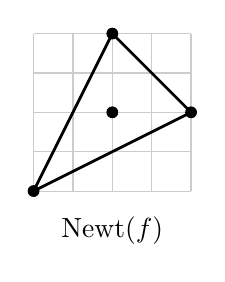
\begin{tikzpicture}[scale=0.5]
		\draw[black!20!white] (0,0) grid (4,4);
		\draw[line width=1pt] (0,0) -- (2,4) -- (4,2) -- cycle;
		\foreach \x/\y in {0/0,2/2,2/4,4/2} {
			\fill (\x,\y) circle (0.15);
		}
		\node at (2,-1) {$\newt(f)$};
		\end{tikzpicture}
		\hspace{10ex}
		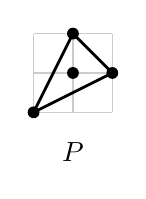
\begin{tikzpicture}[scale=0.5]
		\draw[black!20!white] (0,0) grid (2,2);
		\draw[line width=1pt] (0,0) -- (1,2) -- (2,1) -- cycle;
		\foreach \x/\y in {0/0,1/1,1/2,2/1} {
			\fill (\x,\y) circle (0.15);
		}
		\node at (1,-1) {$P$};
		\end{tikzpicture}
	\end{center}
	
	There are not so many integer points in this triangle: apart from the vertices, it is only the point $(1,1)$. Since $\newt(f_j) \subseteq P$ for every $j \in [r]$, we get 
	\[
		f_j = \sum_{\alpha \in E} c_{j,\alpha} X^\alpha,
	\]
	where 
	\[
		E:= \{(0,0),(1,2),(2,1),(1,1)\}.
	\]
	For the sum of squares we have 
	\[
		f = \sum_{j=1}^r f_j^2 = \sum_{j=1}^r \blue{\sum_{(\alpha, \beta) \in E^2} c_{j,\alpha}c_{j,\beta} X^{\alpha + \beta}. }
	\]
	Thus, if we are interested in expressing a coefficient at the monomial $X^\gamma$ of the polynomial through the coefficients of the $f_j$'s, we need to check for representations $\gamma = \alpha + \beta$ with $\alpha, \beta \in E$. It \blue{is convenient} to view the latter equation as an equation for the midpoints of segments with \blue{points} in $2 E$, by rewriting it as $\gamma = \frac{1}{2}(2 \alpha + 2 \beta)$, where $2 \alpha, 2 \beta \in E$. 
	\begin{center}
		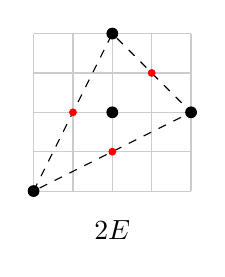
\begin{tikzpicture}[scale=0.5]
		\draw[black!20!white] (0,0) grid (4,4);
		\draw[dashed] (0,0) -- (2,4) -- (4,2) -- cycle;
		\foreach \x/\y in {0/0,2/2,2/4,4/2} {
			\fill (\x,\y) circle (0.15);
		}
		\foreach \x/\y in {1/2,2/1,3/3} {
			\fill[red] (\x,\y) circle (0.1);
		}
		\node at (2,-1) {$2 E$};		
		\end{tikzpicture}
	\end{center}	
	One immediately sees that the only way to obtain the representation $(2,2) = \frac{1}{2} ( 2 \alpha + 2 \beta)$ is by taking both $\alpha$ and $\beta$ equal to $(1,1)$. This shows that $\sum_{j=1}^r c_{j,(1,1)}^2$ is the coefficient of $f$ at the monomial $X^\gamma$ with $\gamma = (2,2)$. But this coefficient is $-3$, and we arrive at $-3 \ge 0$, which is a contradiction. 
	
	(d): The proof of (c) can be used without any changes if $y \ne 1$. If $y=1$, then the Newton polytope of $f$ gets different, because the constant term disappears. In this case, however we see that $f -y $ is not SOS, because $f$ attains negative values. We get $f-1 = X_1^2 X_2^2 (-3 + \blue{X_1^2} + X_2^2)$. So $\blue{f(x_1,x_2) - 1} < 0$ if $x_1,x_2 \in \R \setminus \{0\}$ and the distance of $(x_1,x_2)$ to $(0,0)$ is strictly less than $\sqrt{3}$. 
\end{proof}

\begin{itemize}
	\item \blue{Proposition~\ref{motzkin}}(c) was originally proved without any explicit use of Newton polytopes; see, for example, \cite{Marshall:2008}. The use of Newton polytopes is helpful as it makes the proof idea very clear.
	\item Another useful thing we learn from the proof that uses Newton polytopes is that there is a generalization of the notion of vertex in the world of lattice polytopes (or one can call the world of lattice convex sets, if you like). What we actually proved is the following: if $f$ is SOS and $2P = \blue{\newt(f)}$, then we can define $E = P \cap \Z^n$ and consider the set $2 E$. The set $2E$ is the set of all points of the lattice $(2\Z)^n$ that belong to $\blue{\newt(f)}$. This set $2 E$ has `vertices' (which are the vertices of $\blue{\newt(f)}$) and `generalized vertices', which are points $\gamma$ that cannot be written as $\gamma = \frac{1}{2} (2 \alpha + 2 \beta)$ with $\alpha, \beta \in E$ and $\alpha \ne \beta$. We have essentially shown that if $f$ is SOS and $\gamma$ is a generalized vertex of $2 E$, then the coefficient of $f$ at $X^\gamma$ must be non-negative.
\end{itemize}


Our SDP approach to lower-bounding $f$ does not work at all for $f$ in \blue{Proposition~\ref{motzkin}}, even though $f$ is pretty simple: only two variables and degree six. This $f$ is called the \emph{Motzkin polynomial}. It was discovered by Motzkin. Hilbert was the first to show (in 1888) that SOS is not always equivalent to non-negativity but he didn't give any explicit examples. An explicit example (Motzkin polynomial) was discovered much later, in 1965.

If we allow three variables, we can find a similar polynomial of degree four.

\begin{exercise}
	\label{choi:lam:exer}	
	Show that the following three-variate degree-four polynomial 
	\[
		f = 1 + X_1^2 X_2^2 + X_2^2 X_3^2 + X_1^2 X_3^2 - 4 X_1 X_2 X_3
	\]
	is non-negative, but not SOS. 
\end{exercise} 
\begin{solution}
	To see non-negativity, one can again use the inequality for the geometric and the arithmetic mean: observe that for the four exponent vectors 
	\[
		(0,0,0), (2,2,0),(0,2,2), (2,0,2), (1,1,1)
	\]
	the last one is the arithmetic mean of the remaining ones. 
	For showing that $f$ is not SOS, we can use the Newton polytope of $f$. It can be represented as $2 P$, with $P = \conv( (0,0,0), (1,1,0), (0,1,1), (1,0,1) )$. Here, $P$ is a simplex, and apart from its vertices, there are no other integer points in $P$. If we could write $f$ as $f= f_1^2 + \cdots + f_r^2$, then we had $\newt(f_j) \subseteq P$. Due to the observation about $P$,  $f_j^2$ does not contain the monomial  $X_1 X_2 X_3$. But $f$ does contain this monomial, so we get a contradiction. 
\end{solution}

The polynomial from the previous exercise is called the \emph{Choi-Lam-polynomial}. 

Here are two exercises that illustrate that passing from the dual problem \eqref{unconst:POP:dual:eq} to its SOS-relaxation \eqref{unconst:POP:dual:SOS:eq} one can get a finite positive gap. 

\begin{exercise}
	\label{parrilo:example}
	Consider the homogenization
	\[
	h(X_1,X_2,X_3) := X_3^6 -3 X_1^2 X_2^2 X_3^2 + X_1^2 X_2^4 + X_1^4 X_2^2
	\]
	of the Motzkin polynomial (it is called the \emph{Motzkin form}). Show that 
	\begin{enumerate}[(a)]
		\item $f = h(X_1,1,X_3)$ is non-negative, 
		\item $f$ is not SOS, but 
		\item $h(X_1,1,X_3) +c$ is SOS for some $c \in \R$. 
	\end{enumerate}
\end{exercise}
\begin{solution}
	The examples can be found in \cite[Example~7.2]{Parrilo:2003}.
	\begin{enumerate}[(a)]
	\item Since the Motzkin polynomial $h(X_1,X_2,1)$ is non-negative, also \blue{by Lemma~\ref{homogenization}}, $h(X_1,X_2,X_3)$ is non-negative. Since $h$ is non-negative, then also $f$ is non-negative. 
	\item If $f$ were SOS, then by homogenization of the SOS-representations, we'd get that $h$ is SOS. But then also the Motzkin polynomial $h(X_1,X_2,1)$ would be SOS, which is a contradiction. 
	\item We have
	\[
		f=X_3^6 - 3 X_1^2 X_3^2 + X_1^2 + X_1^4 .
	\]
	The disturbing term here is $- 3 X_1^2 X_3^2$, because its coefficient is negative. We get rid of this term using 
	\[
		X_1^4  - 3 X_1^2 X_3^2 = (X_1^2 - \frac{3}{2} X_3^2)^2 - \frac{9}{4} X_3^4.
	\]
	Thus, we arrive at
	\[
		f = \bigl(X_3^6 - \frac{9}{4} X_3^4 \bigr) + (X_1^2 - \frac{3}{2} X_3^2)^2 + X_1^2
	\]
	The second and third summands are squares. The first summand depends only on $X_3$ and if we add a sufficiently large constant $c$, it becomes non-negative and so SOS. One can for example check that $c=2$ will do (to see that $t^6 - \frac{9}{4} t^4 + 2 \ge 0$ for all $t \in \R$ one can distinguish between $|t| \le 1$ and $|t| \ge 1$ and estimate $t^6$ by~$t^4$ in the latter case).\qedhere
	\end{enumerate}
\end{solution}

\begin{exercise}
	Consider the Motzkin form $h$ from Exercise~\ref{parrilo:example} and the three-variate degree-twelve polynomial 
	\[
		f = (h+1)^2.
	\]
	By construction, $f$ is SOS (in fact, $f$ is a square). Show that $f-1$ is non-negative but not SOS. 
\end{exercise}
\begin{solution}
	The construction (and the solution) was communicated to me by Claus Scheiderer. 
	Observe that $h$ is not SOS. In fact, if $h$ were SOS, then also the Motzkin polynomial $h(X_1,X_2,1)$ would be SOS, which is a contradiction. One has $f - 1= (h+1)^2 - 1 = h (h+2)$, which implies that $f$ is non-negative. To see that $f-1$ is not SOS, note that $f- 1= 2 h + h^2$, where $h$ is homogeneous of degree $6$ and $h^2$ homogeneous of degree $12$. Assume the contrary, $f-1 = 2 h + h^2 = \sum_{j=1}^r g_j^2 + \cdots + g_r^2$ for some $g_1,\ldots,g_r \in \R[X]$. We introduce another indeterminate $Y$  and evaluate the above equality at $(Y X_1, Y X_2, Y X_3)$. Taking into account the homogeneity we get
	\[
		Y^6 2 h(X_1,X_2,X_3) + Y^{12} h(X_1,X_2,X_3) = \sum_{j=1}^r g_j(Y X_1, Y X_2, Y X_3)^2. 
	\]
	Now we can view the left and the right hand sides as elements of $\R[X_1,X_2,X_3][Y]$ (univariate polynomials in $Y$ with polynomials in $X_1, X_2, X_3$ as coefficients). Since the left hand side involves only monomials $Y^6$ and $Y^{12}$,  each $g_j(Y X_1, Y X_2, Y X_3)$ can be written as $Y^3 h_j(X_1,X_2,X_3)$ plus higher order terms (for monomials $Y^4,Y^5,Y^6$). Comparing the coefficients at $Y^6$ we arrive at 
	\[
		2 h(X_1,X_2,X_3) = \sum_{j=1}^r h_j(X_1,X_2,X_3)^2.
	\]
	This contradicts the fact that $h$ is not SOS.
\end{solution}

Also other examples can be generated using the above template (using the Choi-Lam-polynomial, we can construct a four-variate polynomial of degree $8$ with similar properties).

\subsection{Equivalence of non-negativity and SOS for two-variate polynomials of degree four}

There is yet another special situation, where both the degree and the dimensions are fixed to be some specific values, in which non-negativity is equivalent to SOS. If, unlike algebraists, you are not very interested in special degrees and dimensions, you can skip this subsection or read only the formulation of Theorem~\ref{thm:ternary:quartics} below. 

We show that for two-variate polynomials of degree four, SOS is equivalent to non-negativity. The result goes back to Hilbert, but here we follow a different proof recently suggested in the literature. 

\begin{lemma}
	\label{ternary:quartics:lem}
	Let $f \in \R[X]$ be a univariate non-negative polynomial and let $q \in \R[X]$ be a strictly positive quadratic univariate polynomial. Then there exist polynomials \blue{$\eta, \xi \in \R[X]$} such that 
	\[
		f = \eta^2 + q \xi^2.
	\]
\end{lemma}
\begin{proof}
	Changing coordinates and rescaling, we can assume that $q = X^2 + 1$. Since $f$ is non-negative \blue{and w.l.o.g.~non-zero}, its degree is at least two. 
	
	If the degree of $f$ is two, we can write $f$ as $f = (X+a)^2 + b^2$ for some $a,b \in \R$. In this case $\xi^2$ must be a constant, and we show that an appropriate constant can be chosen. We want the constant $\xi$ to be chosen in such a way that $f- q\xi^2$ is a square of a polynomial. Let's compute the coefficients of $f-q \xi^2$:
	
	\begin{align*}
		f - q \xi^2 & = (X+a)^2 + b^2 - (X^2 + 1) \xi^2 
		\\ & = (1-\xi^2) X^2 + 2 a X + a^2 + b^2 - \xi^2.
	\end{align*}
	For $f-q \xi^2$ to be a square of a real polynomial, it is necessary that the coefficient at $X^2$ is non-negative. Thus, we should look for $\xi$ satisfying  $\xi^2 \le 1$. Under this condition, the polynomial $f- q \xi^2$ is a square of a linear polynomial if both its roots coincide, which can be expressed as the discriminant being equal to zero. The discriminant of $f - q \xi^2$ is 
	\[
		\Delta := 4 a^2 - 4 (1-\xi^2) (a^2 + b^2 -\xi^2).
	\] 
	As $\xi^2$ moves from $0$ to $1$, the discriminant $\Delta$ gets changed from $- 4 b^2$ to $4 a^2$. So there is a choice of $\xi^2$ with $\Delta=0$. 
	
	If the polynomial $f$ is of degree larger than two, we use induction. Factorize $f$ as $f=f_1 f_2$, where $f_1$ and $f_2$ are non-constant non-negative polynomials. Such a factorization exists, because $f$ is a product of linear terms and quadratic polynomials (by the fundamental theorem of algebra).
	
	Using the induction assumption for $f_1$ and $f_2$, write each of them in the desired form $f_j = \eta_j^2 + q \xi_j^2$. This gives 
	\begin{align*}
		f & = (\eta_1^2 + q \xi_1^2) (\eta_2^2 + q \xi_2^2) .
	\end{align*}
	We will convert the expression above to the desired form $ f= \eta^2 + q \xi^2$. This can be done just by defining the right $\eta$ and $\xi$ and leaving the comparison of the two expressions as a routine verification. But it would probably be better to have a derivation that is easy to track. So, we'll be using a formal root $\sqrt{q}$ of $q$ (which can be rigorously introduced algebraically) and we will use the root of $-1$, defined by $i^2 = -1$. With this additional objects, we can essentially use the formula $|z_1 z_2| = |z_1| \cdot |z_2|$ for the absolute value of the product of complex numbers $z_1, z_2 \in \compl$ as follows: 
	\begin{align*}
		f & = \bigl(\eta_1^2 + ( \sqrt{q} \xi_1)^2 \bigr) \bigl(\eta_2^2 + (\sqrt{q} \xi_2)^2 \bigr) 
		 \\ & = \bigl | \eta_1 + i \sqrt{q} \xi_1 \bigr|^2 \bigl| \eta_2 + i \sqrt{q} \xi_2 \bigr|^2
		 \\ & = \bigl | (\eta_1 + i \sqrt{q} \xi_1) (\eta_2 + i \sqrt{q} \xi_2) \bigr|
		 \\ & = \bigl| \eta_1 \eta_2 - q \xi_1 \xi_2 + i (\sqrt{q} \xi_1 \eta_2 + \sqrt{q} \xi_2 \eta_1 ) \bigr|
		 \\ & = (\underbrace{\eta_1 \eta_2 - q \xi_1 \xi_2}_{=:\eta})^2 + q ( \underbrace{\xi_1 \eta_2 + \xi_2 \eta_1}_{=:\xi})^2.
	\end{align*}
	This gives a desired expression $ f= \eta^2 + q \xi^2$. In case, one does not believe that the intermediate steps in this calculation have a rigorous mathematical meaning, one could just check that 
	\[
		(\eta_1^2 + q \xi_1^2) (\eta_2^2 + q \xi_2^2) = (\eta_1 \eta_2 - q \xi_1 \xi_2)^2 + q (\xi_1 \eta_2 + \xi_2 \eta_1)^2,
	\]
	is true, which is nothing but checking a polynomial identity. 
\end{proof}

Having this lemma, we can now prove the following. 

\begin{theorem}[Hilbert]
	\label{thm:ternary:quartics}
	Every non-negative two-variate polynomial of degree at most four is SOS. 
\end{theorem}
\begin{proof}
	For the case $n=2, d=4$, the following proof can be given, which is obtained by simplifying the proof in \cite{Pfister:Scheiderer:2012} (see also a related proof in \cite[Prop.~6.3.4]{Bochnak:Coste:Roy:1998}). 
	
	We'll work with homogeneous polynomials in three indeterminates here and we prefer to denote these indeterminates as $X, Y, Z$ in this proof. 
	
	A non-negative two-variate polynomial $g \in \R[X,Y]$ of degree at most four can be homogenized to the three-variate non-negative polynomial $f \in \R[X,Y,Z]$ of degree~$4$ via
	\[
		f(X,Y,Z) := Z^4 g(X/Z,Y/Z).
	\]
%	In terms of exponent vectors, the homogenization from $g$ to $f$ goes by replacing an exponent vector in $\Z_+^2$ with an exponent vector in $\Z_+^3$ by appending a new component so that the sum of the components of the new exponent vector is $4$.
\blue{We have seen in Lemma~\ref{homogenization}}, that whenever $g \ge 0$ on $\R^2$, the homogenization $f$ is non-negative on $\R^3$. Using this operation, we replace the study of arbitrary non-negative polynomials of degree at most $4$ in $2$ indeterminates by a study of homogeneous non-negative polynomials of degree \blue{at most} $4$ in $3$ indeterminates. Let's denote by $C$ the cone of these polynomials 
	\[
		C:= \setcond{ f \in \R[X,Y,Z]}{f \ \text{homogeneous}, f \ge 0 \ \text{on} \ \R^3, \ \blue{\deg(f) \leq 4}}.
	\]
	Clearly, the cone is finite-dimensional, convex and closed. It is also not hard to see that the cone is pointed. To see this, we need to consider $f \in C \cap (-C)$. Such $f$ satisfies $f=0$ on $\R^3$. But, since our underlying domain of coefficients is $\R$,  the latter implies that $f$ is a zero polynomial. Let's recall that a zero polynomial is a polynomial, whose all coefficients are zero. Thus, out of $f(x,y,z) =0$ for all $(x,y,z) \in \R^3$ one needs to conclude that all coefficients of $f$ are zero. This is not particularly difficult but still requires a small argument (we leave the verification as an exercise). 
	
	We know from convexity theory that every vector in a closed pointed convex cone is a sum of finitely many vectors that lie on the extremal rays of the cone. Thus, it suffices to show the assertion for $f$ lying on the extremal ray of $C$.	Consider the unit sphere 
	\[
		S := \setcond{(x,y,z) \in \R^3}{x^2 + y^2 + z^2 = 1}.
	\]
	Due to the homogeneity, the condition $f \ge 0$ on $\R^3$ for homogeneous polynomials can be expressed as $f \ge 0$ on $S$. If a homogeneous polynomial $f$ is strictly positive on $S$, then $f$ would lie in the interior of $C$, as one would have $f+ h \ge 0$ on~$S$ for \blue{every} homogeneous polynomial~$h$ with sufficiently small coefficients. Polynomials in the interior of $C$ are not \blue{contained} in the extremal rays of $C$. So, we can assume that $f \in C$ is equal to zero for at least one $(x,y,z) \in S$. Applying a rotation of $\R^3$ around $(0,0,0)$ we can assume that $f(0,0,1) = 0$. 
	
	We can interpret $\R[X,Y,Z]$ as $\R[X,Y][Z]$ and correspondingly write $f$ as 
	\[
	f(X,Y,Z) = f_0 Z^4 + f_1 Z^3 + f_2 Z^2 + f_3 Z + f_4,
	\] 
	where $f_j \in \R[X,Y]$ is homogeneous of degree $j$, or the zero polynomial. Since $f(0,0,1)=0$, we get $f_0=0$. But then we can also see that $f_1 = 0$. A rigorous way to see this is as follows: We have 
	\[
		0 \le z^{-3} f(x,y,z) = f_1(x,y)  + f_2(x,y) z^{-1} + f_3 z^{-2} \blue{ + f_4 z^{-3}} \to f_1(x,y), \quad \text{as} \ z \to +\infty.
	\]
	This shows $f_1(x,y) \ge 0$, where $f_1$ is a homogeneous polynomial $f_1$ of degree $1$ or equal to $0$. This implies $f_1=0$. 

	Thus, we get
	\[
		f(X,Y,Z) = f_2(X,Y) Z^2 + f_3(X,Y) Z + f_4(X,Y).
	\]
	That is, out of the assumption $f(0,0,1)$ we came to the conclusion that the degree of $f$ with respect to $Z$ is at most two. We proceed by looking at the properties of the `coefficient polynomials' $f_2$ and $f_3$ and $f_4$. Clearly, $f_4 \ge 0$ on $\R^2$ since $f_4(X,Y)= f(X,Y,0)$. On the other hand we have $f_2 \ge 0$ on $\R^2$, which can be shown using an argument similar to the one that we used to show $f_1 \ge 0$ above. We distinguish cases according to the properties of the quadratic form $f_2(X,Y)$.
	
\smallskip
	\emph{Case~1:}	$f_2(X,Y)=0$. Then $f(X,Y,Z) = f_3(X,Y) Z + f_4(X,Y)$ and we must have $f_3 = 0$. Indeed, if we did have $f_3 \ge 0$, then there would be a point $(x,y) \in \R^2$ with $f_3(x,y) \ne 0$. Then $f(x,y,Z)$ is a polynomial of degree one, and we know that a polynomial of degree one cannot be non-negative, which is a contradiction. Hence $f(X,Y,Z) = f_4(X,Y)$. Since $f_4(X,Y) \ge 0$ on $\R^2$, we conclude that $f_4(X,1) \ge 0$ is non-negative on $\R$. \blue{In view of Exercise~\ref{univariate}}, we can write $f_4(X,1)$ as a sum of squares $f_4(X,1) = \sum_{j=1}^r g_j(X)^2$ of polynomials $g_j$ of degree at most two \blue{(actually we could choose $r=2$)}.  Homogenizing this we have 
	\[
		\blue{f(X,Y,Z) = }f_4(X,Y) = Y^4 f_4(X/Y,1) = \sum_{j=1}^r (Y^2 g_j(X/Y))^2,
	\]
	where $Y^2 g_j(X/Y)$ is a homogeneous polynomial of degree two. 	

\smallskip
	\emph{Case~2:} The set of zeros of $f_2$ is a one-dimensional linear space. Then $f_2 = l^2$ for some non-zero linear form $l \in \R[X,Y]$. 	
	\[
		f = l^2 Z^2 + f_3 Z + f_4 .
	\]
	Whenever $(x,y) \in \R^2$ is such that $l(x,y)=0$ holds we get \blue{$f = f_3 Z  + f_4$}. But then $f_3(x,y)=0$ since otherwise, we get a contradiction to $f \ge 0$ in the same way as we did above. It follows that $l(x,y)=0$ implies $f_3(x,y)=0$. This means that~$l$ is a factor of $f_3$. Thus, we can write  $f_3 = 2 l g_2$ for some quadratic polynomial $g_2 \in \R[X,Y]$. Thus, 
	
	\[
		f = (l Z)^2 + 2 g_2 (l Z) + f_4 = (l Z + g_2)^2 + f_4 - \blue{g_2^2. }
	\]
	
	Clearly, \blue{the homogeneous bivariate polynomial} $f_4 - \blue{g_2^2}$ \blue{of degree four} is non-negative (just consider $f(x,y,z)$ for $z= - g_2(x,y) / l(x,y)$ with $l(x,y) \ne 0$, \blue{and use the continuity of polynomials}).
	\blue{Thus, by homogenizing Exercise~\ref{univariate}, it is SOS.}
	It follows that $f$ is SOS. 
	
\smallskip
	\emph{Case~3:} The set of zeros of $f_2$ is $\{(0,0)\}$. Then 
	\begin{equation}
		\label{f2:l1:l2}
		f_2 = l_1^2 + l_2^2
	\end{equation} 
	for some non-trivial linear forms $l_1, l_2 \in \R[X,Y]$. We have a polynomial $f$ which is quadratic in $Z$, and we want to extract a full square with respect to $Z$. For doing this in terms of polynomial coefficients we need to multiply $f$ with an appropriate polynomial: 
	\[
		4 f_2 f = (2 f_2 Z)^2 + 2 f_3 ( 2 f_2 Z) + 4 f_2 f_4 = (2 f_2 Z + f_3)^2 + 4 f_2 f_4 - f_3^2.
	\]
	As above, we see that $4 f_2 f_4 - f_3^2$ is non-negative. Thus, \blue{by applying Lemma~\ref{ternary:quartics:lem} after the dehomogenization $(X,Y) \mapsto (X,1)$ of all involved polynomials, and then homogenizing back again}, there exist bivariate polynomials $\xi(x,y)$ and $\eta(x,y)$ of degrees $2$ and $3$ respectively such that 
	\[
		\eta^2 + \xi^2 f_2 = 4 f_2 f_4 - f_3^2.
	\] 
	This is equivalent to
	\begin{equation}
		\label{eta:f3}
		\eta^2 +f_3^2 = f_2 (4 f_4 - \xi^2). 
	\end{equation}
	Using \eqref{f2:l1:l2}, this can be written as 
	\[
	(\eta + i f_3)(\eta - i f_3) = (l_1 + i l_2) (l_1 - i l_2)( 4 f_4 - \xi^2),
	\]
	where $i^2 = -1$. The polynomials $l_1 \pm i l_2$ have degree one and so they are prime factors. Without loss of generality, we can assume that $l_1 + i l_2$ divides $\eta + i f_3$. Hence,~$f_2$ divides 
	\[
		(\eta+ i f_3) (l_1 - i l_2) = (\eta l_1 + f_3 l_2) + i ( f_3 l_1 - \eta l_2).
	\]
	Since $f_2$ has real coefficients, $f_2$ divides both real and the imaginary part of the latter polynomial. So, the following two fractions are polynomials
	\begin{align*}
		h_1 & := \frac{f_3 l_1 - \eta l_2}{2 f_2} &  h_2 &:= \frac{\eta l_1 + f_3 l_2}{2 f_2}.
	\end{align*}
	By definition of $h_1$ and $h_2$, we have 
	\begin{align*}
		h_1^2 + h_2^2 & = \frac{1}{4 f_2^2} \Bigl((\re ((\eta+i f_3)(l_1-il_2))^2 +  (\im ((\eta+ i f_3)(l_1 - i l_2))^2 \Bigr) 
		\\ & = \frac{1}{4 f_2^2}|(\eta+ i f_3)(l_1 - i l_2)|^2 
		\\ & = \frac{1}{4 f_2^2}|\eta+ i f_3|^2 \cdot |l_1 - i l_2|^2
		\\ & = \frac{(\eta^2 + f_3^2)(l_1^2 + l_2^2)}{4 f_2^2} 
		\\ & = \frac{\eta^2 + f_3^2}{4 f_2} 
		\\ & = f_4 - \frac{1}{4} \xi^2. 
	\end{align*}
	This gives
	\begin{align}
		h_1^2 + h_2^2 & = f_4 - \frac{1}{4} \xi^2. \label{what:is:xi}
	\end{align}
	Moreover, from the definition of $h_1$ and $h_2$ we also have 
	\[
	h_1 l_1 + h_2 l_2 = \frac{f_3 (l_1^2 + l_2^2)}{2 f_2} = \frac{1}{2} f_3.
	\]
	Consequently, 
	\begin{align*}
	(\xi/2)^2 + (h_1 + l_1 Z)^2 + (h_2 + l_2 Z)^2 & \stackrel{\eqref{what:is:xi}}{=} f_4 - h_1^2 - h_2^2 + (h_1 + l_1 Z)^2 + (h_2 + l_2 Z)^2 
	\\ & = f_4 + 2 (\underbrace{h_1 l_1 + h_2 l_2}_{=\frac{1}{2} f_3}) Z + (\underbrace{l_1^2 + l_2^2}_{f_2}) Z^2 
	\\ & = f_2 Z^2 + f_3 Z+ f_4 
	\\ & = f. \qedhere
	\end{align*}
\end{proof}

\blue{
\begin{remark}
The proof above shows that every non-negative two-variate polynomial of degree at most four can be written as a sum of at most three squares.
\end{remark}
}
%
\blue{
\begin{exercise}
(Solution to be found!) Is three squares optimal in the previous remark?
More precisely, does there exist a non-negative two-variate polynomial of degree at most four that needs at least three squares in any SOS representation?
\end{exercise}
}

\begin{exercise}
	Show that $f \in \R[X]$ is a zero polynomial if and only if $f=0$ on~$\R^n$.
\end{exercise} 

\subsection{Non-negativity vs. SOS: Summary}

\begin{theorem}
	Let $d \in \N$ and $n \in \N$. Every $n$-variate \blue{non-negative} polynomial of degree at most $2d$ is SOS if and only if one of the following conditions is fulfilled:
	\begin{enumerate}[(a)]
		\item $n=1$, or
		\item $d=1$, or
		\item $n=2, d=2$.
	\end{enumerate}
\end{theorem}
\begin{proof}
	See results and examples of this chapter (Exercise~\ref{univariate}, Exercise~\ref{degree:two}, Proposition~\ref{motzkin}, Exercise~\ref{choi:lam:exer} and Theorem~\ref{thm:ternary:quartics}).
\end{proof}



	\begin{center}
		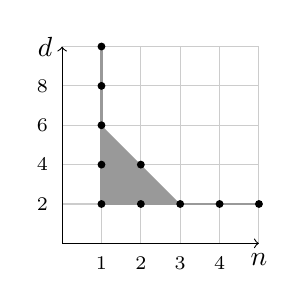
\begin{tikzpicture}[scale=0.5]
		\draw[black!20!white] (0,0) grid (5,5);
		\draw[<->] (5,0) node[below]{$n$} -- (0,0) -- (0,5) node[left]{$d$};
		\foreach \x\y in {1/2,2/4,3/6,4/8} {
			\node at (-0.5,\x) {\scriptsize $\y$};
		}
		\draw[black!40!white,line width=1pt] (1,1) -- (1,5);
		\draw[black!40!white,line width=1pt] (1,1) -- (5,1);
		\fill[black!40!white] (1,1) -- (3,1) -- (1,3) -- cycle;
		\foreach \y in {1,2,3,4} {
			\node at (\y,-0.5) {\scriptsize $\y$};
		}
		\foreach \x/\y in {1/1,2/1,3/1,4/1,5/1,1/2,1/3,1/4,1/5,2/2} {
			\fill (\x,\y) circle (0.1);
		}
		\end{tikzpicture}
	\end{center}	


\begin{remark}
	Similar characterizations were also obtained for symmetric polynomials (invariant up to permutation of variables) and for symmetric polynomials even in each variable; see \cite{choi1977old} and \cite{goel2016choi}.
\end{remark}







\clearpage
\section{Stellensätze with denominators and Hilbert's 17th problem}

In this chapter, too, we deal with $n \in \N$ and indeterminates $X=(X_1,\ldots,X_n)$.

\subsection{Hilbert's 17th problem}

Non-negativity is not equivalent to sos, but can one still certify non-negativity of polynomials algebraically in a different way? This already concerned Hilbert, who included the following problem on his famous list of the 23 problems from the year 1900: is every non-negative polynomial in $\R[X]$ a sum of squares of rational functions?

Recall that we define the field $\R(X)$ of formal quotients $f / g$ with $f, g \in \R[X]$ and $g \ne 0$ with the standard multiplication and addition. 

Artin gave a complete positive solution of Hilbert's problem in 1927, and here we present a `modern version' of Artin's solution. It will turn out that as a byproduct we'll be able to derive a number of Stellensätze, which characterize non-negativity, positivity and equality to zero of a polynomial on a so-called basic closed semialgebraic set.

\subsection{Ordered fields}

We call a subset $P$ of a field $F$ a \emph{preordering} of the field $F$ if $P$ is closed under addition and multiplication, and every square is an element of $P$. That is $x+y \in P$ and $x y \in P$ for all $x, y \in P$ and $x^2 \in P$ for every $x \in F$. By $\sum F^2$ we denote the set of all sums of squares of elements of $F$. Clearly, one has $\sum F^2 \subseteq P$ for every preordering $P$ and $\sum F^2$ itself is a preordering.

If $F$ is a subset of a ring, we'll use the notation $\sum F^2$ for the set of all sums of squares of elements from $F$. For example, $\sum \R[X]^2$ is the set of all sos-polynomials in variables $X$ with coefficients in $\R$ and $\sum \R(X)^2$ is the set of all sums of squares of rational functions in variables $X$.

We call a subset $P$ of $F$ an \emph{ordering} of $F$ if $P$ is closed under addition and multiplication and, furthermore, the equalities $P \cup (-P) = F$ and $P \cap (-P) = \{0\}$ hold. 

\begin{exercise}
	Show that every ordering is a preordering. For this, it suffices to check that if $P$ is an ordering of the field $F$, then every square $x^2$ with $x \in F$ belongs to $P$.
\end{exercise} 
\begin{solution}
	One has either $1 \in P$ or $-1 \in P$. If we had $-1 \in P$, then we also had $(-1) (-1) = 1 \in P$, which is a contradiction. This shows that $1 \in P$. If $x \in F$ and $x \ne 0$, then we either have $x \in F$ or $-x \in F$. In the former case $x^2 \in P$, because $x^2$ is a square of $x$ and in the latter case $x^2 \in P$, because $x^2$ is a square of $-x$. 
\end{solution}

Every ordering $P$ of $F$ defines a total-order relation $\le$ on $F$ given by $x \le y $ if and only if $y -x \in P$.  A field $F$ equipped with $P$ (and the total-order relation $\le$ arising from $P$) is called an ordered field. For an ordered field, one can also introduce $\ge, >$ and $<$ in a natural way. 

\begin{example}
	\label{ex:ordering:rational:functions}
	Let $n=1$ and consider the field $\R(X)$ of univariate rational functions. We order the subfield $\R$ of $\R(X)$ in a standard way ($\R_+$ is the standard ordering of $\R$). Let's order the whole $\R(X)$ by claiming that $X \ge r$ for every $r \in \R$. Once this is required, it is clear how the rest of $\R(X)$ gets ordered. For example, we have $X^2 \ge X$ and $X^3 \ge X$. We also have $1/X < r$ for every $r \in \R$ with $r > 0$. In this ordering $X$ is infinitely large, $X^2$ is even larger, $1/X$ is infinitely small positive, $1/X^2$ is even smaller etc. 
\end{example}

\begin{exercise}
	\label{exer:all:orderings:rational:functions}
	The field $\R(X)$ in the above examples can be ordered in more than one way. 
	\begin{enumerate}[(a)]
		\item Try to find other orderings that extend the ordering of $\R$. 
		\item Can you describe all such orderings? 
	\end{enumerate}
\end{exercise}
\begin{solution}
	(a): Just by interchanging the roles of $X$ and $1/X$, we get another ordering. In this ordering, $1/X$ is infinitely large. One can also require $-X$ to be infinitely large or $-1/X$ to be infinitely large. 
	
	(b): Yet another general possibility (that covers the case of $1/X$ or $-1/X$ being infinitely large) is to fix a number $a \in \R$ and require $X-a$ to be infinitely small positive or infinitely small negative. It is not very hard to convince oneself that the above suggestions cover all possible orderings. In fact, $\R$ is already ordered, and $X$ should occupy some place with respect to the real numbers. We can put it either behind all real numbers or before all real numbers, or fix $a \in \R$ and put $X$ before $a$ or behind $a$ (infinitely close to $a$). 
\end{solution}

We call a field $R$ \emph{real closed} if $R$ is not algebraically closed but $R[\sqrt{-1}]$ is an algebraically closed field. That is, in $R$ we only miss an imaginary unit for representing the roots of polynomial equations. The abstract field $R[\sqrt{-1}]$ is in the same relation to the abstract field $R$ as the field $\mathbb{C}$ of complex numbers to the field $\R$ of real numbers. 

\begin{exercise}
Show the following. For a real closed field $R$, the set  $\sum R^2$ is the unique ordering of $R$. Even more specifically, an element of $R$ is non-negative if and only if it is a square $x^2$ with $x \in R$. 
\end{exercise}
\begin{solution}
	Let $i:= \sqrt{-1}$. Consider an arbitrary ordering of $R$ and let's denote the corresponding order relation (as usual) by $\le$. If $a \in R \setminus \{0\}$ satisfies $a \ge 0$,
	then the equation $\lambda^2 = a$ has two roots in $R[i]$. These roots are either of the form $\pm b$ with $b \in R \setminus \{0\}$ or of the form $\pm i b$ with $b \in R \setminus \{0\}$. In the first case $a = b^2$. In the second case $a = - b^2$. Since $b^2 \ge 0$, we see that in the former case $a \ge 0$ and in the latter case $a \le 0$. Thus, the whole $R$ gets decomposed into squares and `minus squares' (that intersect at the element $0$). This shows that squares are all non-negative elements with respect to our ordering. 
\end{solution}

\begin{theorem}
	\label{thm:extending:to:real:closed}
	For every ordered field $F$ there exists a (unique) real closed extension of $R$. This means $R$ is an extension of the field $F$, $R$ is a real closed field and the set of all elements in $R$ which are non-negative in $R$ and belong to $F$ is exactly the set of all elements of $F$ that are non-negative in $F$. 
\end{theorem}
\begin{proof}
	The proof is contained in \cite{Bochnak:Coste:Roy:1998} (one of the first chapters). 
\end{proof}

\subsection{Quantifier elimination and Tarski's transfer principle}

Let $R$ be a real closed field (for example, $R=\R$).  We start with some terminology
\begin{itemize}
	\item A \emph{boolean formula} is a formula based on and,or,not operations and involving boolean variables (true/false-variables).
	\item A quantifier-free formula $F$ is obtained by plugging in relations of the form $f(X)=0, f(X)>0, f(X) \ge 0$ etc. for $f \in R[X]$ into a boolean formula. So, a quantifier formula depends on indeterminates. If the underlying polynomials have rational coefficients (that is $f \in \Q[X]$), we say that the formula has rational coefficients.
	\item A first-order formula is a formula, in which some of the variables are quantified. It has the form 
	\[
		F(X):= \mathcal{Q}_1 Y_1 \ldots \mathcal{Q}_k Y_k \ \ G(X_1,\ldots,X_n,Y_1,\ldots,Y_k),
	\] where a $G$ is a quantifier free-formula and $\mathcal{Q}_1,\ldots,\mathcal{Q}_k \in \{ \forall, \exists\}$ are quantifiers.
	\item Two formulas $F_1(X)$ and $F_2(X)$ are said to be equivalent over $R$ if $F_1(x)=F_2(x)$ for all $x \in R^n$. 
\end{itemize}


\begin{theorem}[Tarski-Seidenberg quantifier elimination] 
	\label{thm:tarski-seidenberg}
	Let $R$ be a real closed field. Let $F$ be a first-order formula with rational coefficients. Then there exists an algorithm that constructs a quantifier-free formula $G$ with rational coefficients equivalent to $F$. The algorithm depends only on $F$ and not on the choice of the underlying real closed field $R$. 
\end{theorem}
\begin{proof}[About the proof]
	The proof is not particularly hard but a bit long. It proceeds by induction, and one basic thing one should learn to do is counting real roots of a polynomial in an interval (to start the induction). A complete proof can be found in \cite[Th.~1.4.6]{Bochnak:Coste:Roy:1998}. If abstraction is not your favorite activity, one can ready the proof setting $R=\R$, but the point is that for every real closed field $R$ the proof works just the same, and this will turn out to be a \emph{crucial} observation when it comes to proving Stellensätze. 
\end{proof}

Sets defined by a first-order formula are called \emph{semialgebraic}, these are the sets of the form $\setcond{x \in R^n}{F(x)=0}$, where $F(X)$ is a first order formula with free variables $X=(X_1,\ldots,X_n)$. Semialgebraic sets defined by a system of non-strict resp.\ strict polynomial inequalities are called \emph{basic closed} resp.\ \emph{basic open} .

\begin{exercise}
	Let $k,d \in \N$. 
	\begin{enumerate}[(a)]
		\item Is $\cS_+^k$ semialgebraic? Is it basic closed semialgebraic?
		\item Is $\intr(\cS_+^k)$ semialgebraic? Basic open semialgebraic?
		\item Is the set of all non-negative $n$-variate polynomials of degree at most $2d$ semialgebraic?
		\item Is the set of all positive $n$-variate polynomials of degree at most $2d$ semialgebraic?
	\end{enumerate}
\end{exercise}

\begin{remark}[Quantifier elimination algorithms]
	Currently the best quantifier elimination algorithms can carry out the quantifier elimination procedure in $O((m d)^{O(n^{4 (t+1)})})$ arithmetic operations, where $m$ is the number of polynomials involved, $d$ a degree bound and $t$ is the number of quantifier alternations. In particular, if there are no alternations (say, all the quantifiers are existential), the time bound is exponential. In principle, one can solve polynomial optimization problems using quantifier elimination in exponential time (though, no one  would dare to do that on large problems). One reason for the running time being so high, is that in certain situation the output (quantifier-free formula equivalent to the given one) is exponentially large. 
\end{remark}

\begin{remark}[Fourier-Motzkin elimination]
	Fourier-Motzkin elimination is a special case of quantifier elimination occurring in the theory of polyhedra and linear programming. We have a system of affine linear inequalities of the form $f_1(x,y) \ge 0,\ldots,f_m(x,y) \ge 0$ in variables $x \in \R^n$ and $y \in \R$ and we want to write the condition that there exists $y$ satisfying $f_1(x,y) \ge 0,\ldots, f_m(x,y) \ge 0$ in terms of $x$-Variables only. This is possible. The inequalities can be written in the form $y \le u_i(x)$, $y \ge l_j(x)$ and $g_k(x) \ge 0$ with $i \in I$, $j \in J$ and $k \in K$. That is, each inequality either provides an upper bound on $y$, or a lower bound on $y$, or is independent of $y$. Now, the existence of $y$ can be written as the system $\max_{j \in J} l_j(x) \le y \le \min_{i \in I} u_i(x)$, $g_k(x) \ge 0$ for every $k$. The system can be reformulated without any use of $y$ as $l_j(x) \le u_i(x), g_k(x) \ge 0$ for all $i \in I, j \in J, k \in K$. One can see that out of $m$ original inequalities one gets up to $\Theta(m^2)$ inequalities after elimination. There exists examples that show that this cannot be avoided. The situation with a general quantifier elimination is pretty similar. 
\end{remark}

Just to get a feeling how quantifier elimination can be carried out, let us consider a particular example. 

\begin{exercise}
	Compute a quantifier-free formula equivalent to 
	\[
		F(p,q) := \exists x \ \bigl[ \ -1 \le x \le 1 \  \text{and} \ x^2 + p x + q = 0  \ \bigr]
	\]
	Draw a sketch of the respective semialgebraic set $S:= \setcond{(p,q) \in \R^2}{F(p,q) =0}$. 
\end{exercise}
\begin{solution}
	The condition $F(p,q)$ just tells us that the quadratic polynomial $f(X):=X^2 + p X + q$ given by coefficients $p$ and $q$ has a root in the segment $[-1,1]$. Let's figure out how we could characterize this condition in $p$ and $q$ directly, without any use of quantifiers. If the the signs of $f$ at the endpoints of $[-1,1]$ are different, we'll get a root in $[-1,1]$ (by the intermediate value theorem from analysis). So, we'll have a root if $f(-1) \ge 0$ and $f(1) \ge 0$ or $f(-1) \le 0$ and $f(1) \ge 0$. If $f(-1) < 0$ and $f(1) < 0$, we'll have no roots in $[-1,1]$, because $f$ is convex. So, we are left with the case $f(-1) \ge 0, f(1) \ge 0$. Note that the global optimum of $f$ is attained at $x = -p/2$. Thus, $x = -p/2$ is in $[-1,1]$ and $f(-p/2) \le 0$, then $f$ has a root in $[-1,1]$. 
	
	To sum up, if at least one of the following cases occurs, $f$ has a root in $[-1,1]$:
	\begin{enumerate}[(a)]
		\item $f(-1) \le 0, f(1) \ge 0$ or 
		\item $f(-1) \ge 0, f(1) \le 0$ or 
		\item $f(-1) \ge 0, f(1) \ge 0$, $-1 \le -p/2 \le 1$, $f(-p/2) \le 0$.
	\end{enumerate}
	Converse, if neither of the above cases occurs, we must have $f(-1)<0, f(-1) < 0$ or $f(-1) > 0, f(1) > 0$. In the former situation, $f$ has no roots in $[-1,1]$, which follows from convexity of $f$. In the latter situation, if $-p/2$ lies outside $[-1,1]$, then $f$ has no roots in $[-1,1]$ (because $f$ either grows or falls in $[-1,1]$ and remains strictly positive on the whole segment). If $-p/2 \in [-1,1]$, we have $f(-p/2) > 0$ (for, otherwise, the third condition would be fulfilled), which shows that $f$ is strictly positive on $\R$ and thus also on $[-1,1]$. Thus, we have characterized $F(p,q)$ by the above three conditions. In terms of $p$ and $q$ the conditions can be formulated as 
	\begin{enumerate}[(A)]
		\item $1 - p + q \le 0, 1 + p + q \ge 0$ or 
		\item $1 - p + q \ge 0, 1 + p + q \le 0$
		\item $1 - p+ q \ge 0, 1 + p + q \ge 0$, $-1 \le -p/2 \le 1$, $p^2 - 4 q \ge 0$. 
	\end{enumerate}
	Here is a picture of the semialgebraic set described by $F(p,q)$: 
	\begin{center}
		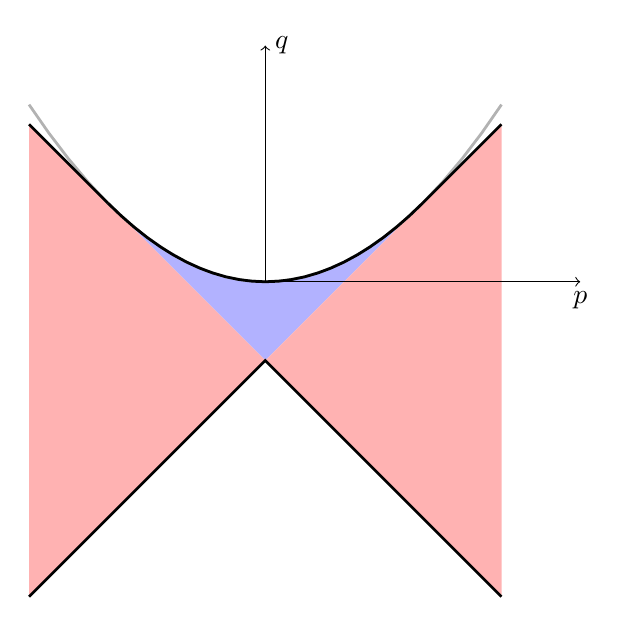
\begin{tikzpicture}
		\fill[blue!30!white,domain = -2:2] plot ({\x}, {\x*\x*0.25}) -- (0,-1); 
		\fill[red!30!white] (0,-1) -- (-3,2) -- (-3,-4) -- cycle;
		\fill[red!30!white] (0,-1) -- (3,2) -- (3,-4) -- cycle;
		
		\draw[black!30!white,domain = -3:3,line width = 1pt,line width = 1pt] plot ({\x}, {\x*\x*0.25});
		\draw[domain = -2:2,line width = 1pt,line width = 1pt] plot ({\x}, {\x*\x*0.25});
		\draw[line width=1pt] (-3,-4) -- (0,-1) -- (3,-4);
		\draw[line width=1pt] (2,1) -- (3,2);
		\draw[line width=1pt] (-2,1) -- (-3,2);
		
		\draw[<->] (0,3) node[right]{$q$} -- (0,0) -- (4,0) node[below]{$p$};
		\end{tikzpicture}
	\end{center}

	This exercise illustrates the following situation. Assume that you are optimizing a function $g(p,q)$ subject to constraints $-1 \le x \le 1$ and $x^2 + p x + q =0$. Even though, it looks as if your feasible set is nice (it is just a piece of a surface described by a simple equation $x^2 + p x + q =0$), projecting out $x$ and writing your constraints without $x$, you see that you are optimizing $g$ over a weird semialgebraic subset of $\R^2$ (which is not basic: it cannot be described by a system of polynomial inequalities). This is in contrast to the situation in linear optimization. In linear optimization, a projection of a polyhedron is a polyhedron again. This exercise shows that a projection of a basic semialgebraic set is not necessarily basic. 
\end{solution}

As a consequence of Tarski's principle, we obtain the following crucial corollary. It says that whenever a first-order formula over $\R$ is satisfiable over a bigger real closed field $R$, then it is also satisfiable over our original smaller field $\R$. 

\begin{corollary}[Tarski's transfer principle]  
	\label{cor:tarski}
	Let $R$ be a real ordered field, which is an ordered extension of the field $\R$. Let $F(X)$ be a first-order formula with coefficients in $\R$. If there exists $x^\ast \in R^n$ such that $F(x^\ast)$ is fulfilled, then there exists also $x' \in \R^n$ such that $F(x')$ is fulfilled. 
\end{corollary}
\begin{proof}
	The proof is borrowed from \cite[Cor.~1.4.7]{Bochnak:Coste:Roy:1998}. It is known that every real ordered field can be extended to a real closed field (see \cite{Bochnak:Coste:Roy:1998}). So, without loss of generality we assume that $R$ is real closed. 
	
	Let $Y=(Y_1,\ldots,Y_k)$ be the quantified variables used in $F(X)$. 
	Each polynomial $f \in \R[X,Y]$ involved in $F(X)$ can be written as $f(X,Y) = g(X,Y,a)$ where $a \in \R^m$ is independent of $f$ and where $g \in \Q[X,Y,Z]$ (a polynomial with rational coefficients) and $Z=(Z_1,\ldots,Z_m)$ are additional indeterminates. For example, if $f(X,Y) = \sqrt{2} X^2 + \sqrt{3} (X-Y) + \sqrt{2} Y^2$ we can introduce $g(X,Y,Z_1,Z_2) = Z_1 X^2 + Z_2 (X-Y) + Z_1 Y^2 \in \Q[X,Y,Z_1,Z_2]$ with $f(X,Y,a) = f(X,Y)$ for $a=(\sqrt{2},\sqrt{3})$.
	
	That is, we put all the real coefficients of all the polynomials involved in $F(X)$ into a vector $a$. This gives rise to a first-order formula $G(X,Z)$ such that $G(X,a) = F(X)$. By Tarski-Seidenberg, $\exists X : G(X,Z)$ can be turned into a quantifier-free form. So, there exists a quantifier-free formula $H(Z)$ with rational coefficients equivalent to $\exists X : G(X,Z)$ over every real closed field. We plug in $Z=a$ and see that $\exists X : G(X,a)$ is equivalent to $H(a)$, where $H(a)$ is independent of $X$ and so $H(a)$ is either true or false. By assumption $\exists X : G(X,a) = \exists X : F(X)$ is true over $R$. So, $H(a)$ is true and so $\exists X : G(X,a) = \exists X : F(X)$ is true over every real closed field containing $\R$ including $\R$ itself. This gives the assertion. 
\end{proof}

\subsection{Solution of Hilbert's 17th problem}

\begin{lemma}[Serre 1947]
	\label{lem:Serre}
	Let $F$ be field of zero characteristic (this means that $\underbrace{1+ \cdots + 1}_k \ne 0$ in $F$ for every $k \in \N$). Let $T$ be a preordering of $F$ and let $f \in F \setminus T$. The inclusion-maximal preordering $P$ with the properties $T \subseteq P$ and $f \not\in P$ is an ordering. 
\end{lemma}
\begin{proof}
	Note that the existence of $P$ follows from Zorn's lemma (and is by this based on the axiom of choice).
	
	We recall that a preodering is a set closed under addition, multiplication and taking squares. We also shortly mention that a preordering is closed under divisions, too. If both $a$ and $b$ are in the preordering and $b$ is not zero, then $a/b = a b (1/b)^2$ and so, we see that immediately.
	
	We first observe that $-1 \not\in P$. In fact, if we had $-1 \in P$, then $P$ is going to be the whole field $F$, which is a contradiction. To see this, it suffices to observe that every element of $F$ is a difference of two squares. Just use the simple identity $ 4 x = (1+x)^2 - (1-x)^2$ and divide it by four (division by four requires $1+1 \ne 0$ in $F$ -- this is the reason of having the assumption on the characteristic of the field $F$). All squares are in the preordering just by definition. If $-1$ is in $P$, then also the minus squares are in the preordering. But then also the differences of the squares are in the preordering and we get $P=F$, which contradicts $f \not\in P$. 
	
	
	We also note that $-f \in P$. If we had $-f \not \in P$, we would get that the set $P - f P$ containing both $P$ and $-f$ is a preordering. In fact, $P - f P$ is closed under addition, because $P$ is closed under addition, $P-f P$ contains all squares, because $P$ contains all squares and $P- f P$ is closed under multiplication, which can be seen by expanding the brackets in $(P -f P)(P - fP)$ and using the fact that $P$ is a preordering. 
	
	Furthermore, since $P$ does not contain $f$, also the set $P - fP$ does not contain $f$. For if $f \in P - fP$, then we had $f = a - f b$ with $a, b \in P$, which gives $(1+b) f = a$. We have $b+1 \ne 0$, since otherwise $-1 = b \in P$ would be an element of $P$. Consequently, $ f= a / (1+b) \in P$, which is a contradiction.
	
	Furthermore, we observe that for every $g \in F$, one has $g \in P$ or $-g \in P$, which means $P \cup (-P) = F$. 
	If, say, $g \not \in P$, we'll show that $-g \in P$. Consider the set $P + g P$. As above, $P + g P$ is a preordering containing $P$, and the containment is proper because $g \in P+ gP$ and $g \not\in P$. By the inclusion-maximality of $P$ under the property $f \not\in P$, we must have $f \in P + gP$, which means that $f = a + g b$ holds for some $a,b \in P$. Then $ - b g = a + (-f) \in P$, because $a \in P$ and we have seen that $-f$ belongs to $P$, too. One cannot have $a - f= 0 $, since otherwise $f = a \in P$. This implies $g b = f -a  \ne 0$. Thus, $b \ne 0$ and by this $-g = (a-f) / b \in P$. 
	
	It remains to show that $P \cap (-P) = \{0\}$ holds. Let $g \in P \cap (-P)$, that is $g, - g \in P$. Then $g =0$, for otherwise, we had $-1 = g (-g) (1/g)^2 \in P$, which contradicts $-1 \not\in P$, which we have derived above. 
\end{proof}

\begin{theorem}[Artin 1927] Let $f \in \R[X]$ be a non-negative polynomial. Then $f \in \sum \R(X)^2$ (that is, $f$ is a sum of squares of rational functions). 
\end{theorem}
\begin{proof}
	Assume to the contrary that $f \not \in \sum \R(X)^2$. Applying the previous lemma to the preordering $\sum \R(X)^2$ of $\R(X)$, we see that there exists an ordering $P$ on $\R(X)$ with respect to which $f$ is negative. We fix $R := \R(X)$ and endow $R$ with the ordering $P$ (this can be viewed as follows: $P$ is a kind of evaluation of rational functions at an `abstract point' and by construction $f$ is strictly negative at this abstract point). By construction, there exists $(x_1,\ldots,x_n) \in R^n$ such that $f(x_1,\ldots,x_n) < 0$. Indeed $X_1,\ldots,X_n$ are rational functions and by this elements of $R$ and so $f(x_1,\ldots,x_n) < 0$ holds for $(x_1,\ldots,x_n) \in R^n$ with $x_1=X_1,\ldots,x_n=X_n$. Since $R$ is a field extending $\R$ and since the coefficients of the polynomial $f$ are in $\R$, Tarski's principle  shows that there also exists $(x_1,\ldots,x_n)$ belonging to $\R^n$ such that $f(x_1,\ldots,x_n) < 0$. This contradicts the non-negativity of $f$. Consequently, $f \in \sum \R(X)^2$. 
\end{proof}

\begin{remark}
The previous proof is not constructive, so it does not provide a method to write a non-negative polynomial as a sum of squares of rational functions. E.g., from the proof, it is not clear \emph{how} the Motzkin polynomial (or other non-sos-polynomials) can be represented as a sum of squares of rational functions. 
\end{remark}

\begin{remark}
	It is known that $2^n$ squares suffice. For $n=1$, we have seen this in our proof. The case $n=2$ is due to Hilbert (1893). The general case is due to Pfister (1965); see \cite{Bochnak:Coste:Roy:1998}. 
\end{remark}

\subsection{An algebraic certificate of non-negativity}

Now, let's consider a more general setting, in which we want to certify whether a polynomial $f$ is positive or non-negative on a basic closed semi-algebraic set $K$. The solution of Hilbert's 17th problems gives a certificate for $K=\R^n$ and, using similar principles, we can also do the case of a more general $K$. 

Given $s$ polynomials $g=(g_1,\ldots,g_s) \in \R[X]^s$, we introduce the basic closed set 
\[
	\{g \ge 0\} := \setcond{x \in \R^n}{g(x) \ge 0}
\]
We'll also use the longer notation
\[
	\{g_1 \ge 0,\ldots, g_s \ge 0\} := \setcond{ x \in\R^n}{g_1(x) \ge 0,\ldots,g_s(x) \ge 0}.
\]
and we'll use an analogous notation for strict inequalities and equalities. With $g$ we also associate
the so-called preordering generated by $g$
\begin{align*}
	\cP(g) & := \cP(g_1,\ldots,g_s) 
	\\ & := \setcond{\sum_{e:=(e_1,\ldots,e_s) \in \{0,1\}^s} \sigma_e g_1^{e_1} \ldots g_s^{e_s} }{ \sigma_e \ \text{sos} \ \text{for every} \ e \in \{0,1\}^s}.
\end{align*}
For example, for $s=2$, $\cP(g_1,g_2)$ consists of polynomials $\sigma_{0,0} + \sigma_{1,0} g_1 + \sigma_{0,1} g_2 + \sigma_{1,1} g_1 g_2$ where $\sigma_{0,0}, \sigma_{1,0}, \sigma_{1,0}, \sigma_{1,1}$ are sos. 

Clearly, $\cP(g)$ is indeed a preordering and it is the inclusion-minimal preordering containing all the polynomials $g_1,\ldots,g_s$. Each $f \in \cP(g)$ is non-negative on $\{g \ge 0\}$. Furthermore, we can recover $\{g \ge 0\}$ from $\cP(g)$ since we obviously have 
\[
	\{g \ge 0\} = \setcond{x \in \R^n}{f(x) \ge 0 \ \text{for all} \ f \in \cP(g)}.
\]
The latter equality allows us to view $\cP(g)$ as a kind of dual object associated to the semi-algebraic set $\{g \ge 0\}$. 

While the condition that $f \ge 0$ on $\{g \ge 0\}$ is a `geometric' non-negativity condition ($f$ non-negative on a semi-algebraic) set, $f \in \cP(g)$ is a sort of `algebraic' non-negativity condition. Though it is not true that the two conditions are equivalent, there is a strong relationship and, for understanding the ideas of the following proofs, it is nice to keep in mind the analogy between the two notions. 

We also introduce the set 
\[
	\cP^0(g):= \cP(g) \cap (-\cP(g))
\]

\begin{itemize}
	\item A representation of $f$ as an element of $\cP(g)$ provides an algebraic evidence for $f \ge 0$ on $\{g \ge 0\}$. 
	\item A representation of $f$ as an element of $\cP^0(g)$ provides an algebraic evidence for $f = 0$ on $\{g \ge 0\}$. 
\end{itemize}

So, it is nice to think of $f \in \cP(g)$ and $f \in \cP^0(g)$ as some kind of `$\ge 0$' and `$=0$' conditions. 

%Sometimes we'll work with sets $F$ that are larger than $\R$, and the we'll use subscript $F$, like $\cP_F(g)$ We will also use notation 

%\[
%	\{ g \ge 0\}_F := \setcond{x \in F^n}{g(x) \ge 0}
%\] 
%for ordered fields extending $\R$ and we'll use the notation like

%\[
%	\cP_F(g) := \setcond{ \sum_{e =(e_1,\ldots,e_s) \in \{0,1\}^s} \sigma_e g_1^{e_1} \cdots g_s^{e_s}}{\sigma_e \in \sum F[X] \ \forall e}
%\]
%where $F$ is a field or ring. 

We recall that an ideal $I$ in a commutative ring $(R,+,\cdot)$ is an additive subgroup of $R$ with the property $I R \subseteq I$. 

\begin{lemma}
	\label{lem:ideals}
	Let $n \in \N$. Let $g=(g_1,\ldots,g_s) \in \R[X]^s$, let $P:=\cP(g)$ and $I:=\cP^0(g)$. Then the following hold: 
	\begin{enumerate}[(a)]
		\item \label{I:ideal} $I$ is an ideal of $\R[X]$.
		\item \label{I:proper} If $I$ is proper (that is $I \ne \R[X]$), then $-1 \not\in P$ (analogy: if there is an element not equal to zero `in the abstract sense', the constants like $-1$ are not non-negative `in the abstract sense').
		\item \label{sum:non-neg:zero} If $p, q \in P$ and $p+q \in I$, then $p, q \in I$ (analogy: if the sum of non-negative elements is zero, then all the summands are zero). 
	\end{enumerate}
\end{lemma}
\begin{proof}
 \eqref{I:ideal}: Since $P$ is closed under addition, $I$ too is closed under addition. Since $0 \in P$ we have $0 \in I$ and it is clear that $I + I = I$. For every $f \in I$ also $-f \in I$. So $(I,+)$ is a subgroup of $\R[X]$. Let $q \in I = P \cap (-P)$. As we did above, we use a formula telling us that every element of a $\R[X]$ is a difference of two squares.
 
 For every $p \in \R[X]$, one has $ 4 p = (1+p)^2 - (1-p)^2$. Since $(1+p)^2 q \in P \cap (-P)$ and $(1-p)^2 q \in P \cap (-P)$, we conclude that $4 p q \in P \cap (-P)$. Dividing by $4$, we get $p q \in P \cap (-P)$. Here is a bit more detailed explanation how we can get the conclusion: From $q \in P$ and $-q \in P$, we get $(1+p)^2 q \in P$ and $-(1-p)^2 q \in P$, respectively. This yields $(1+p)^2 q - (1-p)^2 q \in P$, meaning $4 p q \in P$. Dividing by $4$, we get $p q \in P$. Completely analogously, we also get $p q \in -P$. 
 
 \eqref{I:proper}: If $-1 \in P$, then using $ 4 p = (1+p)^2 - (1-p)^2$, we conclude that $P = \R[X]$. Hence $I=P \cap (-P) = \R[X]$, which is a contradiction. 
 
 \eqref{sum:non-neg:zero}: Since, $p,q \in P$, we have $p+q \in P$. So we just need to show $-p, -q \in P$. Indeed, showing this, we get $-(p+q) \in P$ and conclude $p+q \in P \cap (-P) = I$. By $p+q \in I$ we have $-p - q \in P$. So $-p \in q + P \subseteq P$ and $-q  \in p +P \subseteq P$. 
\end{proof}

An ideal $\cP^0(g)$ should help us certify the condition $f=0$ on $\{g \ge 0\}$. However, $\cP^0(g)$ may have an undesired property of being non-prime. Here is just a small example with $g=(g_1,g_2)$, $g_1=X_1 X_2, g_2 = -X_1 X_2$. In this case, the set $\{g \ge 0\} = \{X_1 X_2 = 0\}$ is just the union of two coordinate axes. The polynomial $X_1$ does not belong to $\cP(g)$, because $X_1$ is not non-negative on $\{g \ge 0\}$. Analogously, the polynomial $X_2$ does not belong to $\cP(g)$ because $X_2$ is not non-negative on $\{g \ge 0\}$. It is clear that the product $X_1 X_2$ belongs to $\cP^0(g)$. So, we conclude that neither $X_1$ nor $X_2$ belongs to $\cP^0(g)$ but their product $X_1 X_2$ does belong to $\cP^0(g)$. This shows that the ideal $\cP^0(g)$ is not prime. The reason of $\cP^0(g)$ being non-prime is the fact that the variety $\{X_1 X_2 = 0\}$ is not irreducible. 

In the proof of our positivstellensatz  we'll need a step of enlarging $\cP^0(g)$ to a prime ideal (which dually can be viewed as picking an irreducible component in a variety). 


\begin{exercise}
	\label{powers:prime:ideals}
	Show that, if $J$ is a prime ideal and $m \in \N$, then $p^m \in J$ implies $p \in J$.
\end{exercise}
\begin{solution}
	For $m=1$ this is clear. If $m \ge 2$, then $p p^{m-1} \in J$ and since $J$ is prime, $p$ or $p^{m-1}$ is in $J$. In the former case, we get the desired assertion. In the latter case, by induction, we deduce that $p \in J$.
\end{solution}

\begin{lemma}
	\label{lem:prime:ideals}
	In the notation of Lemma~\ref{lem:ideals}, we have 
	\begin{enumerate}[(a)]
		\item If $I$ is a proper subset of $\R[X]$ and if $J$ is a minimal prime ideal containing $I$, then, for all $p,q \in P$ satisfying $p, q \in P$ and $p+q \in J$, one has $p, q \in J$. 
		\item For the ideal $J$ in (a) and the field $F$ of fractions over the integral domain $\R[X] / J$, the set
		\[
			P' := \setcond{ \sum_{e \in \{0,1\}^s} \sigma_e g^e }{\sigma_e \in \sum F^2}.
		\] 
		is a proper preordering of $F$.
	\end{enumerate}
\end{lemma}
\begin{proof} See \cite[Prop.~2.1.7]{Marshall:2008}. 
 (a): It is known that there exists an inclusion-minimal prime ideal $J \subseteq \R[X]$ with $I \subseteq J$ (follows by applying Zorn's lemma to the family of all prime ideals that contain $I$ as a subset). It is also known that in this case for every $p \in J$, there exists an integer $m \ge 0$ and an element $q \in \R[X] \setminus J$ with $p^m q \in I$; see any basic book in commutative algebra, for example, \cite[Prop.~1.14]{Atiyah:Macdonald:2016}. Here is an illustration in the context of number theory of how this works. The ideal $12 \Z$ is contained in two inclusion-minimal prime ideals $2 \Z$ and $3 \Z$. If we raise an element of $2 \Z$ to the power two and then multiply with $3 \not\in 2 \Z$, we get an element of $12 \Z$. An illustration in terms of polynomial rings is as follows. The ideal $X_1^4 X_2 \R[X_1,X_2]$ is contained in two prime ideals $X_1 \R[X_1,X_2]$ and $X_2 \R[X_1,X_2]$. Taking a fourth power of an element of $X_1 \R[X_1,X_2]$ and multiplying it with $X_2 \not\in X_1 \R[X_1,X_2]$, we get an element of $X_1^4 X_2 \R[X_1,X_2]$. 
 
 So, if $p+q \in J$, then $(p+q)^n u \in I$ holds for some $n \ge 0$ and $u \not\in J$. This gives $u^2 (p+q)^n \in I$. We can always assume that $n$ is odd. If $n$ is even, just increase $n$ by one, by multiplying with $(p+q)$.  Using binomial expansion we can write $u^2 (p+q)^n$ as a non-negative linear combination of the terms $u^2 p^i q^{n-i}$ with $i \in \{0,\ldots,n\}$. Depending on whether $i$ is odd or even, we can write the latter term as a square multiplied by $p$ or a square multiplied by $q$. So we conclude that $u^2 (p+q)^n$ is an element of $I$ which can be written as a sum of terms belonging to $P$. By Lemma~\ref{lem:ideals}(c), every term $u^2 p^i q^{n-i}$ belongs to $I$. In particular also $u^2 p^n \in I$. Since $I \subseteq J$, $J$ is prime and $u \not \in J$, we get $p \in J$. Indeed, $u^2 \not \in J$ since $u \not\in J$ and $J$ is prime (see Exercise~\ref{powers:prime:ideals}). Then from $u^2 \not\in J$ and $u^2 p^n \in J$, we deduce that $p^n \in J$ (since $J$ is prime). From $p^n$ we deduce $p \in J$ (see Exercise~\ref{powers:prime:ideals}). Since $p$ and $q$ play the same roles, we also get $q \in J$. 

(b): This is related to \cite[Prop.~2.1.6]{Marshall:2008}. Assume the contrary, that is, $P'= F$. Then $-1 \in P'$. This means
\[
	-1 = \sum_{e \in \{0,1\}^s} \sigma_e g^e 
\]
for some $\sigma_e \in \sum F^2$, $g^e := g_1^{e_1} \cdots g_s^{e_s}$ and $e=(e_1,\ldots,e_s)$. Note that $F$ is a field of fractions over the integral domain $\R[X]/J$. The terms $\sigma_e$ are sums of squares of fractions of elements of $\R[X]/J$. So, setting $f$ to be the product of all the denominators in the mentioned fractions, we get
\[
	-f^2 = \sum_{e \in \{0,1\}^s} \sigma_e g^e
\]
for some $\sigma_e \in \sum (\R[X]/J)^2$ and $f \in R[X]/J$ with $f \ne 0$ in $\R[X]/J$. The latter identity can be written as an identity modulo $J$. So, coming from $\R[X] / J$ to $\R[X]$, this gives
\[
	-f^2 \in \underbrace{\sum_{e \in \{0,1\}^s} \sigma_e g_e}_{=:h} + J. 
\]
for some $f \in \R[X]$ and $f \not\in J$ and some choices $\sigma_e \in \sum \R[X]^2$. 

We have thus shown $h + f^2 \in J$. Here, $h \in P$ by construction, and $f^2 \in P$, because $f^2$ is a square. By (a), we conclude $f^2 \in J$. Since $J$ is prime, we get $f \in J$, which is a contradiction. 
\end{proof}


\subsection{A Farkas-type lemma for polynomial inequalities}

\begin{theorem}[Certifying infeasibility of a polynomial system; a Farkas Lemma for POP] 
	\label{thm:farkas:pop}
	Let $g = (g_1,\ldots,g_s) \in \R[X]^s$. Then $\{g \ge 0\} = \emptyset$ if and only if $-1 \in \cP(g)$. 
\end{theorem}
\begin{proof}
	The sufficiency is clear, so we need to prove the necessity. Assume $-1 \not\in \cP(g)$. We will prove that $\{g \ge 0\}$ is non-empty. Consider the ideal $I := \cP^0(g)$. Since $\cP(g) \supseteq I$, we have $-1 \not\in I$, that is, $I$ is a proper subset of $\R[X]$. There exists a prime ideal $J$ containing $I$ as a subset and being minimal with respect to inclusion with respect to this property. Let $F$ be the field of fractions of $\R[X]/J$. The preordering $P'$ from Lemma~\ref{lem:prime:ideals} is a proper subset of $F$ and so, using Lemma~\ref{lem:Serre}, we can find an ordering $P$ with $P \supseteq P'$. With the ordering $P$, the field $F$ becomes an ordered field. Consider the natural homomorphisms $f \mapsto f+J \mapsto \frac{f+J}{1}$ on the spaces $\R[X] \to \R[X] / J \to F$. These homomorphisms send $X_1,\ldots,X_n \in \R[X]$ to some $x_1,\ldots,x_n \in F$. By construction, we have $g_1(x_1,\ldots,x_n) \ge 0,\ldots g_s(x_1,\ldots,x_n) \ge 0$ for the constructed $(x_1,\ldots,x_n) \in F^n$ (with respect to the ordering $P$ we've fixed for $F$). Thus, we found a solution of the system $g \ge 0$ in the space $F^n$. By Tarski-Seideberg transfer principle (Corollary~\ref{cor:tarski}), there exists also a solution in $\R^n$. 
\end{proof}

\begin{remark}
	A representation of $-1$ as an element of $\cP(g)$ is an infeasibility certificate for the system $g_1(x) \ge 0,\ldots,g_s(x) \ge 0$. This theorem does not provide a direction control of the size of such a certificate, as there is nothing mentioned about the degree of the sos-polynomials $\sigma_e$ in the representation $-1 = \sum_{e \in \{0,1\}^s} \sigma_e g^e$. Tools from real algebra allow to show that such a certificate is realizable with degrees of the polynomials $\sigma_e$ bounded in terms of $n$ and the degrees of $g_i$'s only, but it is likely that such degree bounds for $\sigma_e$ are necessarily very huge. 
\end{remark}


\subsection{Stellensätze with denominators}

The following theorem contains a Positivstellensatz (positive-locus theorem), a Nichtnegativstellensatz (non-negative-locus theorem) and a Nullstellensatz (zero-locus theorem). 

\begin{theorem}[{Krivine 1964, Stengle 1974; see \cite[Thm.~2.2.1]{Marshall:2008}}]
	\label{stellensaetze}
	Let $g = (g_1,\ldots,g_s) \in \R[X]^s$, let $K = \{ g \ge 0\}$ and $P= \cP(g)$. Then for $f \in \R[X]$ the following conditions hold.
	\begin{enumerate}[(a)]
		\item $f>0$ on $K$ if and only if there exist $p, q \in P$ with $p f = 1+ q$. 
		%
		\item $f \ge 0$ on $K$ if and only if there exists an integer $m \ge 0$ and $p, q \in P$ such that $p f = f^{2m} + q$. 
		%
		\item $f=0$ on $K$ if and only if there exists an integer $m \ge 0$ such that $-f^{2m} \in P$. 
	\end{enumerate}
\end{theorem}
\begin{proof}
	(a): The sufficiency is easy: if $p f = 1+q$, then there exists no $x \in K$ with $f(x) \le 0$: if $g(x) \ge 0$ and $f(x) \le 0$, then $p(x) f(x) = 1+q(x)$ yields a contradiction, because the left hand side is $\le 0$ and the right hand side is $> 0$. Conversely,  if $f>0$ on $K$, then $\{ g \ge 0,-f \ge 0 \}$ is empty and so by the  Theorem~\ref{thm:farkas:pop} (the `polynomial Farkas-lemma'), we know that $-1 \in \cP(g,-f)$. Clearly, $\cP(g,-f) = \cP(g) - f \cP(g) = P - f P$ and so we get $-1 = q - f p$ for some $q, p \in P$, which is exactly what we need to derive. 
	
	(b): Sufficiency : if $p f = f^{2m} +q$ then there exists no $x \in K$ with $f(x) < 0$: if we had $g(x) \ge 0$ and $f(x) < 0$, then $f^{2m}(x) + q(x) > 0$ and $p(x) f(x) \le 0$, which is a contradiction. Conversely, assume $f \ge 0$ on $K$. We assume $f \ne 0$ as otherwise the assertion is clear. We'll get to the situation of (a) using lifting. Condition $f \ge 0$ on $\{g \ge 0\}$ can be phrased as $f > 0$ on $\{ g \ge 0, f \ne 0\}$. We can rewrite $f(X) \ne 0$ as $f(X) Y =1$ using an addition indeterminate $Y$. This gives $f > 0$ on $\{ g(X) \ge 0, f(X) Y =  1\} \subseteq \R^{n+1}$. Rewriting the equality condition through inequality gives $f> 0$ on $\{g(X) \ge 0, 1 - f(X) Y \ge 0, f(X) Y - 1 \ge 0\}$. By (a), we get 
	$p(X,Y) f(X) = 1+ q(X,Y) $ with $p, q \in \cP(g,1-f(X) Y, -1 + f(X) Y)$. Substituting $Y = 1/f(X)$. This gives $p(X,1/f(X)) f(X) = 1 + q(X,1/f(X))$. Multiplying through by a sufficiently large power $f(X)^{2m}$ of $f(X)$ clears the denominators and we get the desired assertion. 
	
	(c): Sufficiency: if $- f^{2m} \in P$, then there exists no $x \in K$ and $f(x) \ne 0$: indeed, for such $x$ we would have $- f^{2m}(x) < 0$, but the condition $-f^{2m} \in P$ tells us that one has $-f^{2m}(x) \ge 0$, which is a contradiction. Conversely, if we have $f = 0$ on $K$, then $f \ge 0$ on $K$ and $f \le 0$ on $K$ and we can use the argument of (b). We have $p_1 f = f^{2m} + q_1$ and $p_2 (-f) = f^{2m} + q_2$ for some $p_1,p_2,q_1, q_2\in P$ (using the same $m$ in both relations is possible, as we can see from the proof of (b)). Multiplication of both equalities yields $-p_1 p_2 f^2 = f^{4m} + (q_1+q_2) f^{2m}  +q_1 q_2$. So we see that $-f^{4m} \in P$.   
\end{proof}

\subsection{Remarks on Stellensätze}

	\begin{enumerate}[(a)]
		\item Positive solution of Hilbert's 17th problem says that the condition $f(X) \ge 0$ can be characterized algebraically as $f \in \sum \R(X)^2$. Theorem~\ref{stellensaetze}(b) gives yet another certificate: $f(X) \ge 0$ iff $p f = f^{2m} + q$ for some $p, q \in \SOS{\R[X]}$ and some integer $m \ge 0$. It turns out that the certificate of (b) is in a way stronger, as we can convert it to the $\SOS{\R(X)}$-certificate as follows. Assume $f \ne 0$ (as otherwise, things are clear). In this case $p$ is not a zero polynomial as well, since the right hand side $f^{2m} + q$ is not a zero polynomial. So we can rewrite $p f = f^{2m}+ q$ as $f = \frac{1}{p} (f^{2m} + q)$ and, rewriting this as $f = (\frac{1}{p})^2 p ( f^{2m} + q)$, we see that $f \in \SOS{\R(X)}$.
		\item What happens when we consider equality constraints, say $g=0$ rather than $g \ge 0$? Rewriting $g=0$ as $g \ge 0, -g \ge 0$, we can use Theorem~\ref{stellensaetze}. A polynomial $f$ is positive on $\{g=0\}$ if and only if $p f = 1+q$, where $p,q \in \cP(g,-g)$. Note however that every polynomial is a difference of two squares. This shows that $\cP(g,-g) = \SOS{\R[X]} + I$, where
		\[
			I = \R[X] g_1 + \cdots + \R[X] g_s
		\]
		is the so-called ideal generated by $g_1,\ldots,g_s$. Thus, working with equality constraints we have a particularly simple certificate of positivity. This observation can be extended to non-negativity condition and to the case where both inequality and equality constraints are present. 
		\item In the classical algebraic geometry (over an algebraic field like complex numbers), one would try to describe polynomials that vanish on an $\{g=0\} = \{g_1=0,\ldots,g_s=0\}$. We want can characterize  $f=0$ on $\{g=0\}$ algebraically. By Theorem~\ref{stellensaetze}(c), we've got $-f^{2m} \in \cP(-g,g)$. Since $\cP(g,-g) = \SOS{\R[X]} +I$, with $I$ as above, we have the certificate $-f^{2m} = \SOS{\R[X]} +I$ for the condition $f = 0$ on $\{g=0\}$. This is analogous to the Nullstellensatz from classical algebraic geometry. 
		\item Of course, one may wonder whether one really needs denominators. Our intention was to describe the preordering 
		\[
		\Tilde{\cP}(g):=\setcond{f \in \R[X]}{f(x) \ge 0 \ \text{on} \ \{g \ge 0\}}
		\] 
		and we would prefer a simple description if possible. Theorem~\ref{stellensaetze} gives one such description, which is quite involved: the certificate $p f = f^{2m} + q$ involves two polynomials $p$ and $q$ and an integer $m \ge 0$. So, it would be nice if we had, say $\Tilde{\cP}(g)=\cP(g)$. Unfortunately, this equality doesn't always hold. We have seen, this equality does not hold for every $n \ge 2$  if we have no constraints. It's known that when $n \ge 3$ and $\{g \ge 0\}$ has non-empty interior, we've got just the same situation, namely $\Tilde{cP}(g) \ne \cP(g)$ . This means that characterizing non-negativity on $\{g \ge 0\}$ algebraically is not an easy task. Strict positivity is characterized in a nicer way. Computationally, dealing with strict positivity rather than non-negativity we do not lose much. Apart from that, for posivitity, in a number of cases there are denominator-free certificates (this is the topic of the following chapter).
		\item One serious difference to the Farkas lemmas from linear programming is that the degree of sos-polynomials in our certificates can be extremely large. The maximum degree has not been estimated exactly so far. But there is an extremely huge upper bound that has recently been established in \cite{lombardi2014elementary}. It was shown that if a polynomial $f$ of degree $d$ is non-negative on $\R^n$, then $q f = p$, where $q,p$ are sos-polynomials of degree at most 
		\[
			2^{2^{2^{d^{4^n}}}}.
		\]
		I do not know, up to what extent the bound can be improved. 
		\item Stellensätze could have also been derived with respect to an arbitrary real closed field. This has imporatant quantitative consequences in the spirit of the previous remark. Real algebraic geometry contains results that give us as a corollary of the latter fact that the degrees of the polynomials $p,q \in \cP(g)$ involved in the certificates can be bounded in terms of $n$, and the degrees of $f$ and $g_1,\ldots,g_s$. However, the theory does not tell us what the bounds exactly are. 
	\end{enumerate}




\clearpage 
\section{Positivstellensätze without denominators}

Let $X=(X_1,\ldots,X_n)$ be indeterminates and $n \in \N$. Consider the basic semi-algebraic set $\{g \ge 0\}$ given by $g =(g_1,\ldots,g_s) \in \R[X]^s$.  The template questions of this chapter are: Does the condition $f > 0$ on $\{g \ge 0\}$ imply that $f \in \cP(g)$? Can one use another set rather than $\cP(g)$ in such a context? We'll see positive answers in a number of situations and provide links to linear and semidefinite programming.
The presentation in this chapter is based on \cite{averkov2013constructive}.

%\subsection{Affine version of Farkas lemma}

%Recall that $\blue{\cone(M)}$ is the convex conic hull of \blue{$M$}. One of the basic Nichtnegativstellens\"atze without denominators is the Farkas lemma. Its affine version can be formulated as follows.
%We say that a polynomial is linear if its degree is at most one. 
%
%\begin{lemma}[Affine version of Farkas lemma]
%	\label{lem:farkas}
%	Let $f,a_1,\ldots,a_m \in \R[X]$ be $n$-variate linear polynomials, and let the polyhedron $K = \{a_1 \ge 0,\ldots a_m \ge 0\} \subseteq \R^n$ be non-empty.
%	Then the following conditions are equivalent:
%	\begin{enumerate}[(i)]
%		\item $f \ge 0$ on $K$
%		\item $f \in \cone(1,a_1,\ldots,a_m)$. 
%	\end{enumerate}
%\end{lemma}
%\begin{proof}
%	Exercise
%\end{proof}


\subsection{P\'olya: a positivstellensatz on a simplex}

The templates for the following results will be: if $f > 0$ on a compact set $K$, then there exists some algebraic representation of $f$ providing the evidence that $f \ge 0$ on $K$. So, you see that it is not a characterization, but an implication: you require strict positivity and have the evidence for non-negativity only. Such results can of course be converted into a characterization of positivity. It suffices to invoke the above implication for $f - \eps$ in place of $f$, where $\eps>0$ is small enough so that $f - \eps$ is still positive on $K$. 


The following theorem is about homogeneous polynomials, which are positive on the standard simplex.
For dealing with exponent vectors of homogeneous polynomials, we introduce the notation 
\[
	\bE^n_d := \setcond{\alpha \in \Z_+^n}{|\alpha | =d}.
\]
We also use the notation $\alpha ! = \alpha_1 ! \cdot \ldots \cdot \alpha_n !$ for $\alpha = (\alpha_1,\ldots,\alpha_n) \in \Z^n_+$.


\begin{theorem}[P\'olya 1928] 
	Let $f \in \R[X]$ be a homogeneous polynomial, with $f> 0$ on the simplex 
	\[
		\Delta := \setcond{(x_1,\ldots,x_n) \in \R_+^n}{x_1 + \cdots + x_n =1}.
	\]
	Then there exists $N \in \Z_+$ such that all coefficients of $(X_1 + \cdots + X_n)^N f(X)$ are non-negative. 
\end{theorem}
\begin{proof}

	We write $f$ as $\sum_{\alpha \in \bE^n_d} c_\alpha X^\alpha$. The expression $(X_1 + \cdots + X_n)^N$ can be expanded so that we get
	\begin{align*}
		 g & := (X_1+ \cdots + X_n)^N f 
		 \\ & = \sum_{\beta \in \bE^n_N} \frac{N!}{\beta !} X^\beta \sum_{\alpha \in \bE^n_d} c_\alpha X^\alpha 
		 \\ & = \sum_{\alpha \in \bE^n_d, \beta \in \bE^n_N} c_\alpha \frac{N!}{\beta!} X^{\alpha+\beta}.
	\end{align*}
	
	We see that $g$ is a homogeneous polynomial of degree $d+N$:
	\[
		g = \sum_{\gamma \in \bE^n_{d+N}} A_\gamma X^\gamma
	\]
	whose coefficients can be expressed through the coefficients of $f$ by:
	\begin{equation}
		\label{A:gamma:first:eq}
		A_\gamma = \sum_{\alpha \in \bE^n_d \,:\, \alpha \le \gamma} c_\alpha \frac{N!}{(\gamma-\alpha)!} .
	\end{equation}
	We want to analyze the behavior of $A_\gamma$ for growing $N$. To this end, we factor out an appropriate term in the above sum describing $A_\gamma$:
	\[
		A_\gamma = \frac{N!(N+d)^d}{\gamma!} \sum_{\alpha \in \bE^n_d \, : \alpha \le \gamma} c_\alpha \frac{\gamma !}{(\gamma-\alpha)! (N+d)^d}.
	\]
	In the latter sum, the coefficients $c_\alpha$ are multiplied by values depending on $N$. In order to see how these values behave for $N \to \infty$, we express them differently. Since both $\gamma!$ and $(\gamma-\alpha)!$ are products of $n$ factorials and since $|\alpha|=d$, we get
	\[
		\frac{\gamma!}{(\gamma-\alpha)! (N+d)^d} = \prod_{i=1}^n \frac{\gamma_i !}{(\gamma_i-\alpha_i)! (N+d)^{\alpha_i}} ,
	\]
	where $\alpha = (\alpha_1,\ldots,\alpha_n)$ and $\gamma=(\gamma_1,\ldots,\gamma_n)$. The quotient $\gamma_i! / (\gamma_i-\alpha_i)!$ is the product of the $\alpha_i$ many values $\gamma_i-\alpha_i+1,\ldots,\gamma_i$. Hence 
	
	\[
		\frac{\gamma_i !}{(\gamma_i-\alpha_i)! (N+d)^{\alpha_i}} = \left(\frac{\gamma_i - \alpha_i+1}{N+d} \right) \cdots \left( \frac{\gamma_i}{N+d} \right).
	\]
	Summarizing this gives
	\[
		A_\gamma = \frac{N!(N+d)^d}{\gamma!} \sum_{\alpha \in \bE^n_d \, : \alpha \le \gamma} c_\alpha \prod_{i=1}^n \left(\frac{\gamma_i - \alpha_i+1}{N+d} \right) \cdots \left( \frac{\gamma_i}{N+d} \right).
	\]
	We can discard the condition $\alpha \le \gamma$  and let the sum go over all $\alpha \in \bE^n_d$, for if $\alpha_i > \gamma_i$ for some $i \in [n]$, then the respective term in the product occurring in the latter representation of $A_\gamma$ is equal to zero. 
	
	In this context, it will be convenient to use the notation
	\[
		(x)_t^m := x (x-t) \cdots x (x - (m-1) t).
	\]
	Note that for $t \to 0$, $(x)_t^m \to x^m$, so for small $t$, the value $(x)_t^m$ is a perturbed version of $x^m$. In this notation $A_\gamma$ can be represented as
	
	\[
		A_\gamma = \frac{N!(N+d)^d}{\gamma!} \sum_{\alpha \in \bE^n_d} c_\alpha \left(\frac{\gamma_1}{N+d} \right)_{1/(N+d)}^{\alpha_1} \cdots  \left(\frac{\gamma_n}{N+d} \right)_{1/(N+d)}^{\alpha_n}.
	\]	
	Since one has $|\gamma|= N+d$, we get $\gamma / (N+d) \in \Delta$. Consider the polynomial
	
	\[
		f_t(X) = \sum_{\alpha \in \bE^n_d} c_\alpha (X_1)_t^{\alpha_1} \cdots (X_n)_t^{\alpha_n}.
	\]
	
	The polynomial function $f_t(x)$ converges to $f(x)$ uniformly on $\Delta$ as $t \rightarrow 0$ (recall that the uniform and the pointwise convergence are equivalent for continuous functions on a compact set). Thus, \blue{by our assumption that $f > 0$ on $\Delta$}, we get $f_t(x)>0$ for all $x \in \Delta$ if $t$ is small enough. Up to a positive multiple, our $A_\gamma$ coincides with $f_t(\gamma/ (N+d))$ for $t=\frac{1}{N+d}$. It follows that $A_\gamma  > 0$ for all $\gamma$, if $N$ is large enough. 
\end{proof}

\begin{remark}
\blue{
The proof above shows that for large enough $N$ every possible monomial $X^\gamma$, for $\gamma \in \bE^n_{d+N}$, appears in $(X_1 + \dots + X_n)^N f(X)$ with a positive coefficient.}

\blue{As an example consider the polynomial $f = X^2 - 2 X Y + 2 Y^2 = (X - Y)^2 + Y^2$ which is positive on~$\Delta \subseteq \R^2$.
We have
\[
(X+Y)^4 f(X) = X^6 + 2 X^5Y + 5 X^2Y^4 + 6 XY^5 + 2Y^6,
\]
in which every coefficient is non-negative, but not every monomial of degree six appears.
However, in $(X+Y)^6 f(X)$ every monomial of degree six appears and has a positive coefficient.
}
\end{remark}

\begin{remark}
	Quantitative aspects of P\'olya's theorem (how large is $N$, depending on $f$) were investigated by Reznick \& Powers \cite{Powers:Reznick:2001}. They give a choice of $N$ depending on $d,n$ and $\min_{x \in \Delta} f(x)$. Their paper also contains a complete proof of P\'olya's theorem. 
\end{remark}

\subsection{P\'olya's theorem and copositivity} 

A symmetric matrix $A \in \cS^n$ is called co-positive if $\sprod{x}{A x} \ge 0$ holds for all $x \in \R_{\ge 0}^n$. This means the quadratic polynomial $f(x) = \sprod{x}{A x}$ is non-negative on the standard simplex $\Delta$. If $\sprod{x}{Ax}>0$ holds for all $x \ne 0$, then $A$ is called strictly copositive and the corresponding quadratic polynomial $f(x)$ is strictly positive on the standard simplex. P\'olyas theorem addresses strict positivity as a special case. Checking whether a matrix is copositive (strictly copositive) is hard. This can also be seen from the fact that a number of NP-hard problems can be formulated as conic problems over the copositive cone (conic problems will be the topic of Chapter~\ref{conic:optimization}; roughly, a conic program is a problem of optimization of a linear objective function over an affine slice of a given cone). See also the survey \cite{dur2010copositive}. Copositive programming is a special case of inequality constrained quadratic programming. 


\subsection{P\'olya's theorem and the cone of homogeneous polynomials} 

Let's denote by $\oP_{n,d}(\Delta)$ the closed convex cone of all homogeneous $n$-variate polynomials of degree $d$ that are non-negative on the simplex $\Delta$. P\'olyas theorem provides a sequence of polyhedral cones $\oP_{n,d}^N(\Delta)$ approximating the cone $\oP_{n,d}(\Delta)$ arbitrarily well, as $N \to \infty$. In fact, the condition that all coefficients of $(X_1+\cdots +X_n)^N f$ are non-negative is a system of linear inequalities for the coefficients of $f$. The polynomial $f$ occurs linearly in the expression $(X_1+\cdots + X_n)^N f$, or to put it a bit differently, the map $f \mapsto (X_1+ \cdots +X_n)^N f$ is linear. For $N=0$, the condition is just that all coefficients of $f$ are non-negative. Thus, for $N=0$, the set $\oP_{n,d}^N(\Delta)$ is just a simplicial cone. For large $N$ explicit inequalities on the coefficients of $f$ can be found in the proof. By \eqref{A:gamma:first:eq}, the inequalities are 
	\begin{align*}
		\sum_{\alpha \in \bE^n_d \,:\, \alpha \le \gamma} c_\alpha \frac{1}{(\gamma-\alpha)!} & \ge 0 & & \forall \gamma \in \bE^n_{N+d}.
	\end{align*}


\begin{example}
	To illustrate this, we consider approximations of the copositive cone for $n=2$.  We consider a quadratic form $f(x,y)$ given as $f(x,y) = a x^2 +  b x y + c y^2$. So, in this case $\oP_{n,d}(\Delta)= \oP_{2,2}(\Delta)$ is a three-dimensional cone. It will be more convenient for us to look at the slices of the cone and so we fix a normalization \blue{$2 a + b + 2 c = 2$} of coefficients of $f$, which corresponds to slicing $\oP_{2,2}(\Delta)$ by a hyperplane (the slice by the hyperplane $a + b + c=1$ is unbounded, see Exercise~\ref{ex:polya:unboundedslice} below). It is known, and \blue{sketched in Exercise~\ref{ex:polya:P22decomposition} below}, that the cone $\oP_{2,2}(\Delta)$ is generated by the polynomial $xy$ and the PSD quadratic forms (that is, each $f\in \oP_{2,2}(\Delta)$ is $f = \alpha g + \beta xy$, where $\alpha, \beta \ge 0$ and $g$ is PSD). Note that $f$ is PSD if and only if $a \ge 0, c \ge 0, a c - (\frac{b}{2})^2 \ge 0$ holds (this is a basic fact in linear algebra). We look at the equality $a c - (\frac{b}{2})^2 =0$ which, in view of $2a + b + 2c = 2$, can be formulated as $a c - (1- (a+c))^2 = 0$. This equation describes an ellipse tangent to the $a$ and $c$ axes and lying in the non-negative orthant. 
	
	The best is to write the condition in $a+c$ and $a -c$. Using $\xi=a+c$ and $\eta = a-c$ and multiplying by $4$, this can be formulated as
	\[
		\xi^2 - \eta^2 - 4 (1- \xi)^2 = 0.
	\]
	This is
	\[
		- 3 \xi^2  + 8 \xi - 4 - \eta^2 = 0
	\]
	which gives
	\[
		3 \xi^2 - 8 \xi + 4 + \eta^2 = 0
	\]
	and can be written as
	\[
		3 (\xi - 4/3)^2 + \eta^2 = \frac{4}{3}.
	\]
	So we get an equation of the ellipse (that is, the boundary of the PSD forms sliced by $2a + b + 2c = 2$ is an ellipse). We remark that from $a c - (1 - (a+c))^2 = 0$ one gets $a \ge 0$ and $c \ge 0$. Furthermore both $a =0$ and $c=0$ are possible (by choosing $a=0, c=1$ and $a=1, c = 0$). Here is a picture of it generated with WolframAlpha:
	\begin{center}
		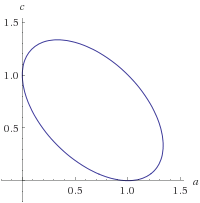
\includegraphics[width=150pt]{sdp_ellipse}
	\end{center}
	
	\blue{The full slice of $\oP_{2,2}(\Delta)$ is then given by the convex hull of this ellipse and the origin, which can be seen by scaling a general form $\alpha g + \beta xy$ back to the chosen hyperplane $2a + b + 2c = 2$.}
	Here is a picture, generated by Benjamin Peters using Matlab that shows how (the slices of) $\oP_{2,2}^N(\Delta)$ approximate (the slice of) $\oP_{2,2}(\Delta)$.
	
	\begin{center}
	\begin{tikzpicture}[]
	\pgftext{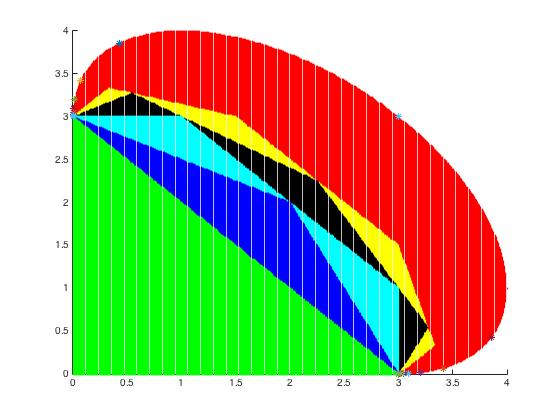
\includegraphics[width=150pt]{polya_polyhedra}} at (0pt,0pt);
	\end{tikzpicture}
	\end{center}

	As $N$ grows, $\oP_{2,2}^N(\Delta)$ is growing larger and larger so that every interior point of the red region is eventually covered. But for some of these points it takes very long to be covered. 
\end{example}

\begin{exercise}
	\label{ex:polya:unboundedslice}
	Show that the slice of 
	\[
		\oP_{2,2}(\Delta) := \setcond{(a,b,c) \in \R^3}{f:=a x^2 + b x y + c y^2 \ge 0  \ \text{on} \ \Delta}
	\] 
	by the hyperplane $a+b+c=1$ is unbounded. 
\end{exercise}
\begin{solution}
	Clearly, the slice is non-empty, because all $(a,b,c)$ with $a + b + c=1$ and $a,b,c \ge 0$ are in the slice. It suffices to find $(a',b',c') \in \oP_{2,2}(\Delta)$ with $a' + b' +c'=0$. Adding arbitrary non-negative multiples of this to any point of the slice we do not fall out of the slice. This shows that a slice contains a ray and so is unbounded. As we know from the convexity theorem, unboundedness of a closed convex set can always be certified by providing a ray that is contained in the set. Finding such an element is easy: $(x-y)^2 = x^2 - 2xy + y^2$ is non-negative ant it yields $a'=1, b'=-2$ and $c'=1$. Done!
\end{solution}

%\begin{exercise*}
%	 Determine all hyperplane slices of $P_{2,2}(\Delta)$ which are non-empty and bounded. UNDER CONSTRUCTION: At this point the exercise may come too early as duality of cones has not been discussed, yet. 
%\end{exercise*}
%\begin{solution}
%	psd quadratic forms are in $P_{2,2}(\Delta)$ and $xy$ is also in $P_{2,2}(\Delta)$. This allows to see that $P_{2,2}(\Delta)$ is the sum of two cones $K_1 + K_2$, where $K_1$ are quadratic forms with non-negative coefficients and $K_2$ are psd quadratic forms. So if slicing $K_1$ or $K_2$, we get an unbounded set, we have unboundedness. One can also show the converse, if both slice of $K_1$ and slice of $K_2$ is bounded, then also the slice of $K_1 + K_2$ will be bounded (standard convexity). 
%	UNDER CONSTRUCTION
%\end{solution}

\begin{exercise}
	\label{ex:polya:P22decomposition}
Show that $\oP_{2,2}(\Delta)$ is the convex conic hull of all psd quadratic forms $q(x,y)$ and the polynomials $xy$.
\end{exercise}

\begin{solution}	
(Sketch of the solution)
%
Clearly, the mentioned convex conic hull is a subset of $\oP_{2,2}(\Delta)$. To prove the converse, it suffices to show that every point on an extremal ray of $\oP_{2,2}(\Delta)$ is psd quadratic form or coincides with $xy$ up to a multiple. Note that $\oP_{2,2}(\Delta)$ is pointed and full-dimensional. Every point $f$ on the extremal ray is on the boundary ans so has a zero in $\Delta$. If it has a zero in the relative interior of $\Delta$ it is a square and so a psd form. If it has a zero in an endpoint of $\Delta$, there are the following cases. If both endpoints are zeros of $f$, then $f$ coincides with $xy$ up to a non-negative multiple. If only one endpoint is zero, then we tweak on $f$ so that it remains non-negative on $\Delta$ using $x^2$ or $y^2$. This shows that $f$ is not extremal.
\end{solution}


\subsection{Handelman: a positivstellensatz on a polytope} 

P\'olya's theorem can be used to derive a positivstellensatz on polytopes.

For $a_1,\ldots,a_m \in \R[X]$ and $a=(a_1,\ldots,a_m)$ we introduce the semiring generated by $a$ as 
\[
	\cS(a) := \setcond{\sum_{e=(e_1,\ldots,e_m) \in E} c_e a_1^{e_1} \cdots a_m^{e_m} }{c_e \in \R_{\ge 0} \ \forall e \in E, \ E \subseteq \Z_+^m \ \text{finite}}.
\]
The set $\cS(a)$ consists of conic combinations of products of powers of $a_1,\ldots,a_m$. It is clear, that a representation of $f$ as an element of $\cS(a)$ gives a certificate for non-negativity of $f$ on $\{a \ge 0\}$. 

\begin{remark}[P\'olya on general simplices]
P\'olya's theorem applied in a straightforward way yields a positivstellensatz on an arbitrary simplex. If $a_1,\ldots,a_{n+1}$ are linear polynomials and $S:=\{a_1 \ge 0,\ldots, a_{n+1} \ge 0\}$ is an $n$-dimensional simplex, then every polynomial $f$ strictly positive on $S$ belongs to $\cS(a)$. The sketch of the argument is as follows. Up to rescaling, one can assume $a_1 + \cdots + a_{n+1} = 1$. The original variables $X_1,\ldots,X_n$ can be expressed through $a_1,\ldots,a_{n+1}$, which will become our `new variables', and if $f$ has degree at most $d$, we can replace each monomial in~$f$ by a homogeneous polynomial of degree $d$ in `new variables' $a_1,\ldots,a_{n+1}$. After this, applying P\'olya's theorem, we get the desired conclusion. 
\end{remark}

\blue{We need two ingredients to extend P\'{o}lya's result to arbitrary polytopes.
For the first, let }$f \in \R[X]$ be a polynomial of degree at most $d$ and let~$l \in \R[X]$ be a linear homogeneous polynomial.
Then, $g = l^d f (X/l)$ is a polynomial, too. Moreover, $g$ is a homogeneous polynomial and we call it a \emph{homogenization} of $f$ with respect to $l$.

Let's see an example for how this kind of homogenization works. If  say $f = X_1 + X_1 X_2 + X_1 X_2 X_3^2$ and $l=X_1 + X_2 +X_3$, then the degree of $f$ is $4$. There is a monomial of degree one and a monomial of degree two. We multiply each of these monomials by an appropriate power of $l$ to get the homogeneous polynomial
\[
	g = X_1 l^3 + X_1 X_2 l^2 + X_1 X_2 X_3^2. 
\]

\blue{The second ingredient is one of the basic Nichtnegativstellens\"atze without denominators -- the Farkas lemma.
Recall that $\cone(M)$ is the convex conic hull of $M$.
We say that a polynomial is linear if its degree is at most one.}
%
\blue{\begin{lemma}[Affine version of Farkas lemma]
	\label{lem:farkas}
	Let $f,a_1,\ldots,a_m \in \R[X]$ be $n$-variate linear polynomials, and let the polyhedron $K = \{a_1 \ge 0,\ldots, a_m \ge 0\} \subseteq \R^n$ be non-empty.
	Then, the following conditions are equivalent:
	\begin{enumerate}[(i)]
		\item $f \ge 0$ on $K$
		\item $f \in \cone(1,a_1,\ldots,a_m)$. 
	\end{enumerate}
\end{lemma}
\begin{proof}
	Exercise
\end{proof}
}

\begin{theorem}[Positivstellensatz of Handelman]
	Let $a = (a_1,\ldots,a_m) \in \R[X]^m$ be polynomials of degree at most one and let the polyhedron $S:= \{a \ge 0\}$ defined by the inequalities $a \ge 0$ be non-empty and bounded. Then every polynomial $f \in \R[X]$ strictly positive on $S$ belongs to $\cS(a)$. 
\end{theorem}
\begin{proof}
	Without loss of generality, we can assume that $S \subseteq \R_{\ge 0}^n$ (because we can translate $S$ into the non-negative orthant $\R_{\ge 0}^n$, and translation is just an affine change of coordinates in the space $\R^n$). 
	
	Every polynomial is bounded on \blue{the compact set} $S$ so that the polynomial $X_1 + \cdots + X_n + a_1(X) + \cdots +a_m(X)$ has an upper bound $t \in \R_{> 0}$ on $S$. Let 
	\[
		q = t - (X_1 + \cdots + X_n) - (a_1(X) + \cdots + a_m(X)).
	\] 
	By construction $q \ge 0$ on $S$. We introduce new indeterminates $Y = (Y_1,\ldots,Y_m)$ and $Z$ and the polynomials 
	\[
		\sigma = \frac{1}{t} ( X_1 + \cdots + X_n + Y_1 + \cdots +Y_m + Z)
	\]
	and
	\[
		g = f(X) + c \sum_{i=1}^m (a_i(X) - Y_i)^2
	\]
	in these indeterminates. Here, $c \in \R_{>0}$ is a constant that will be fixed in what follows. 
	
	Let $\Delta$ be the simplex given by 
	\[
		\Delta:=\setcond{(x,y,z) \in \R_{\ge 0}^{n+m+1}}{\sigma(x,y,z) = 1}.
	\]
	The $\Delta$ is up to rescaling a standard simplex (and so it is as good as a standard simplex for our purposes).
	Let $A$ be the subset of $\Delta$ given by 
	\[
		A = \setcond{(x,y,z) \in \Delta}{a_i(x) = y_i \ \forall i \in [m]}.
	\]
	The polynomials $f$ and $g$ coincide on $A$ and \blue{$a_i(x) = y_i \geq 0$, for all $i \in [m]$ on~$A$.
	Hence, $f = g > 0$ on $A$.} Above, we've lifted our~$f$ to a polynomial $g$ in a larger space and in that larger space, the positivity of~$f$ on the original set $S$ is translated to the positivity of $g$ on $A$. 
	
	Since $\blue{g} > 0$ on $A$, $\blue{g}$ is also positive on a small compact neighborhood of $A$. In $\Delta$ and outside this small neighborhood, $g$ can be made arbitrarily large, by choosing $c>0$ sufficiently large. Indeed, if we are away from $A$, the sum occurring in the definition of $g$ can be bounded from below by a positive constant and so, choosing the factor $c$ in the definition of $c$ sufficiently large we can ensure that $g> 0$ on the whole $\Delta$. Clearly, one can construct a homogeneous polynomial $g_0$ such that $g=g_0$ on $\Delta$: Just homogenize $g$ with respect to $\sigma$, by setting $g_0 := \sigma^{\deg g} g( X / \sigma, Y / \sigma, Z / \sigma)$. 
	
	Applying P\'olya's theorem to $g_0$, we get that for some large enough integer $N \in \Z_+$ all coefficients of $\sigma^N(X,Y,Z) g_0(X,Y,Z) $ are non-negative. Substituting $Z = t - (X_1 + \cdots + X_n) - (Y_1 + \cdots + Y_m)$, the polynomial $\sigma$ is turned to $1$. Subsequent substitutions $Y_i = a_i(X)$, turn the polynomial $g$ to $f$. We thus, conclude that
	$f = g_0(X,a_1(X),\ldots,a_m(X), q(X))$ is in the semiring  \[
		\cS(X_1,\ldots,X_m,a_1(X),\ldots,a_m(X),q(X)).
	\] Note that $X_1,\ldots,X_m, q(X)$ do not contribute to this semiring, because by Farkas' lemma (Lemma~\ref{lem:farkas}), these polynomials of degree at most $1$ are in $\cone(1,a_1,\ldots,a_m)$. This shows that the latter semiring coincides with $\cS(a)$. So, the assertion follows.
\end{proof}


\subsection{Handelman's theorem and linear programming}

Let's borrow the notation $a=(a_1,\ldots,a_m)$ and $S$ of Handelman's theorem and let $f \in \R[X]$ be arbitrary. In view of Handelman's theorem, the polynomial optimization problem
\[
	\min \setcond{f(x)}{a \ge 0}
\]
over the polytope $S= \{a \ge 0\}$ has the dual formulation 
\[
	\max \setcond{y \in \R}{f - y \ge 0  \ \text{on} \ S} = \sup \setcond{y \in \R}{f - y \in \cS(a)}.
\]
We really need to pass to the supremum, because Handelman's theorem is a positivstellensatz (it is about `strict' positivity). Now we can modify this problem by replacing the whole $\cS(a)$ by its truncated version
\[
	\cS_E (a) := \setcond{ \sum_{e \in E} c_e a^{e_1} \cdots a^{e_m}}{c_e \ge 0 \ \forall e \in E} \,,
\]
where $E \subseteq \Z_+^m$ is finite and fixed. The problems
\begin{equation}
	\label{handelman:relaxation}
	\max \setcond{y}{f - y \in \cS_E(a)}
\end{equation}
give lower bounds on the original minimization problem. In view of Handelman's theorem, the hierarchy of such problems with, say, $E=E^m_d$ and $d \in \N$ gives optimal values that converge to the optimal value of the original problem, as $d$ grows. Unfortunately, the convergence may be quite slow (because Handelman is based on P\'olya and so it inherits the convergence problems of P\'olya).

Let's also note that \eqref{handelman:relaxation} is a \emph{linear} problem. The objective is linear (it's just one variable $y$). The constraint $f -y \in \cS_E(a)$ is the linear equality system 
\[
	 y+ \sum_{e=(e_1,\ldots,e_m) \in E} c_e a_1^{e_1} \cdots a_m^{e_m} = f
\]
for the decision variable $y \in \R$ and the non-negative decision variables $c_e \in \R_{\ge 0}$. Indeed, the $c_e$'s and $y$ occur linearly in this expression. The polynomial $f$ is the right hand side. 

\begin{remark}
	Applicability of Handelman-based approaches (including analysis of convergence etc.) has been discussed in several sources. 
\end{remark}

\subsection{Quadratic modules and constrained polynomial optimization} 

\label{quadr:modules:pop}

If $a=(a_1,\ldots,a_s) \in \R[X]^s$ are arbitrary polynomials, then the set 
\[
	\cM(a):= \setcond{g_0 + g_1 a_1 + \cdots + g_s a_s}{g_0,\ldots,g_s \ \text{are SOS} }
\]
is called the quadratic module generated by $a=(a_1,\ldots,a_s)$. Thus, the general constrained polynomial optimization problem, \blue{with objective function $f \in \R[X]$,}
\begin{equation}
	\label{constr:pop}
	\inf \setcond{f(x)}{x \in \R^n, a_1(x) \ge 0,\ldots, a_s(x) \ge 0}
\end{equation}
over the set $\{a \ge 0\}$
can be relaxed to
\begin{equation}
	\label{module:relax}
	\sup \setcond{y \in \R}{f - y\in \cM(a)}.
\end{equation}
In fact, the supremum is a lower bound on the infimum, because the elements of $\cM(a)$ are non-negative on $\{a \ge 0\}$. The condition $f - y \in \cM(a)$ can be formulated as a semidefinite constraint. For this purpose it will be convenient to introduce the family $\cS^\infty$ of infinite-size symmetric matrices with only finitely many non-zero entries. For such matrices $A \in \cS^\infty$ the PSD property can be defined in the usual way. So, we also have a PSD cone $\cS_+^\infty$ in that space. Let 
\[
	m(X) = (X^\alpha)_{\alpha \in \Z_+^n}
\] 
be the infinite vector containing all possible monomials $X^\alpha$. 

A polynomial $g$ is SOS if and only if $g=m(X)^\top Z m(X)$, where $Z = (z_{\alpha,\beta})_{\alpha,\beta \in \Z_+^n}$ is PSD. Thus, the condition $f - y \in \cM(a)$ can be written as 

\begin{equation}
 f(X) - y = m(X)^\top Z_0 m(X) + \sum_{j=1}^s a_j(X) m(X)^\top Z_j m(X),
 \label{eq:quadr:mod:conditions}
\end{equation} 
where $Z_0,\ldots,Z_s \in \cS_+^\infty$ are infinite PSD matrices, whose entries are indexed by exponent vectors $\alpha = (\alpha_1,\ldots,\alpha_n) \in \Z_+^n$. Thus, our relaxed problem \eqref{module:relax} is the infinite SDP
\begin{equation}
	\label{inf:sdp}
	\sup \setcond{y \in \R}{Z_0,\ldots,Z_s \in \cS_+^\infty, \ y + m(X)^\top Z_0 m(X) + \sum_{j=1}^s a_j(X) m(X)^\top Z_j m(X) =f(X)} \,.
\end{equation}
The latter problem can be modified to a finite problem, since $\cS_+^\infty$ essentially contains $\cS_+^k$ for every $k$. That is, the latter problem can be truncated to the problem 
\begin{equation}
	\label{trunc:module:realax}
	\sup \setcond{y \in \R}{Z_0,\ldots,Z_s \in \cS_+^k, \ y + m_d(X)^\top Z_0 m_d(X) + \sum_{j=1}^s a_j(X) m_d(X)^\top Z_j m_d(X) = f(X)},
\end{equation}
where $m_d(X) = (X^\alpha)_{\alpha \in E_d^n}$, $d \in \N$ \blue{and $k = |E^n_d|$}. It is clear that the optimal value of~\eqref{trunc:module:realax} is a lower bound on the optimal value of~\eqref{inf:sdp} and one can approximate the optimum of \eqref{inf:sdp} arbitrarily well by choosing $d$ sufficiently large.

In what follows we try to establish cases of equivalence of \eqref{constr:pop} and \eqref{module:relax} by deriving positivstellensätze that are based on quadratic modules. 

\begin{remark}[What kind of certificate should we prefer?]
	So far, we've seen several sets used for certifying positivity and leading to various relaxations of polynomial optimization. The sets are 
	\begin{itemize}
		\item the semiring $\cS(a)$ (used in Handelman's theorem when the $a_j$'s are linear),
		\item the quadratic module $\cM(a)$ (introduced above),
		\item the preordering $\cP(a)$ (can also be used just in the same way as $\cM(a)$ was used above). 
	\end{itemize}
	Which of them can one use? Which of them are the better ones? As for the first question, there is a guarantee of convergence of the respective hierarchies if we have established a respective stellensatz (though, convergence may be really slow). As for the second question, comparison of such sets is not an obvious matter. Assume that $f>0$ on $\{a \ge 0\}$ and we can certify non-negativity of $f$ on $\{a \ge 0\}$ by representing it as an element of $\cM(a)$ and also by representing it as an element of $\cP(a)$. Will the representation as an element of $\cM(a)$ be shorter? This is not really clear! Note that both representations would involve SOS-polynomials and we do not know much about their degrees. 
\end{remark}


\subsection{Positivstellensätze involving quadratic modules}

In this section, we'll see that quadratic modules yield positivstellens\"atze on bounded sets, if we add an additional special polynomial to the generators of the underlying quadratic module. As a consequence, we'll also see that the assertion of Handelman's theorem remains true if we replace $\cS(a)$ by $\cM(a)$. 

\begin{exercise}
	\label{prop:prod:pm:product}
	Show the following: Let $X_1,\ldots,X_n,Y_1,\ldots,Y_n$ be indeterminates. Let $E_+^n$ and $E_-^n$, respectively, be the set of all vectors $e \in \{-1,1\}^n$ with an even resp. odd number of entries equal to $-1$. Then 
	\[
		X_1 \cdot \ldots \cdot X_n \pm Y_1 \cdot \ldots \cdot Y_n = \frac{1}{2^{n-1}} \sum_{e \in E_\pm^n} \prod_{i=1}^n (X_i + e_i Y_i).
	\]
	In particular, $X_1 \cdot \ldots \cdot X_n \pm Y_1 \cdot \ldots \cdot Y_n$ belong to the semiring generated by $X_1+Y_1,\ldots,X_n+Y_n,X_1 - Y_1,\ldots,X_n-Y_n$. 
\end{exercise}
\begin{solution}
	Induction on $n$. 
\end{solution}

\begin{lemma} \label{lem:t:minus:squares}
	Let $f \in \R[X] = \R[X_1,\ldots,X_n]$ and let $\rho > 0$. Then, there exists $t \in \R$ such that $t + f$ and $t- f$ belong \blue{to $\cP(\rho - \|X\|^2)$, that is, }to the preordering generated by $\rho - \|X\|^2 = \rho - (X_1^2 + \cdots + X_n^2)$. 
\end{lemma}
\begin{proof} 
\blue{Write $f = \sum_\alpha c_\alpha X^\alpha$.}
	We use $t = \sum_\alpha |c_\alpha| (\rho+1)^{|\alpha|}$. Since the definition of $t$ does not depend on changing $f$ to $-f$ (because $|c_\alpha| = |-c_\alpha|$), it suffices to check the assertion for $t + f$. We have 
	\[
		t+ f = \sum_\alpha |c_\alpha| ( (\rho+1)^{|\alpha|} + \sign(c_\alpha) X^\alpha) .
	\]
	\blue{If $\alpha = 0$, then the corresponding term in $t+f$ is $|c_0|(\rho+1+\sign(c_0)) \geq 0$.}
	For $\alpha \ne 0$, we apply Exercise~\ref{prop:prod:pm:product} to  $(\rho+1)^{|\alpha|} \pm X^\alpha$ and conclude that $t+f$ is in the semiring generated by all $\rho+1 \pm X_i$ with $i \in [n]$. Now, it suffices to see that $\rho+1 \pm X_i$ is in the preordering generated by $\rho - \|X\|^2$. Due to the symmetry we can assume $i=1$. Since changing $X_1$ to $-X_1$ does not change $\|X\|^2$, it suffices to look at $\rho + 1 + X_1$. We have
	\[
		\rho+1 + X_1 = \frac{1}{2} \bigl( (\rho+1) + (1+X_1)^2 + X_2^2 + \cdots + X_n^2  + (\rho - \|X\|^2) \bigr) \,.\qedhere
	\]
\end{proof}
%
\blue{Observe that, if $t \in \R$ is a valid choice in Lemma~\ref{lem:t:minus:squares}, then every $\bar t \geq t$ also satisfies $\bar t \pm f \in \cP(\rho - \|X\|^2)$.}
%
The following lemma will be applied in the case $\{a \ge 0 \} \subseteq B$ by choosing $B$ to be a large box. 
\begin{lemma} \label{lem:transfer}
	Let $a=(a_1,\ldots,a_s) \in \R[X]^s$ and let $f \in \R[X]$ be strictly positive on $\{a \ge 0\}$. Let $B \subseteq \R^n$ be compact. Then there exists $g \in \cM(a)$ such that $f - g $ is strictly positive on $B$. 
\end{lemma}
\begin{proof}
	The set \blue{$a(B):= \setcond{\left(a_1(x),\ldots,a_s(x)\right)}{x \in B} \subseteq \R^s$ is the image of a continuous function of a compact set, and is thus compact.}
	So there exists \blue{$\gamma > 0$} with $a(B) \subseteq (-\infty, 2 \gamma]^s$. Consider $T:= \setcond{x \in B}{f(x) \le 0}$. Since $f> 0$ on \blue{the closed set} $\{a \ge 0\}$, we get $a(T) \cap [-2 \eps, 2 \gamma]^s = \emptyset$ for a sufficiently small $\eps>0$. This can also be formulated as the inequality $f(x) > 0$ being fulfilled for all $x \in B$ satisfying $a_i(x) \ge -2 \eps$ for all $i \in [s]$. We now introduce the univariate polynomial $h(t) := t \left( \frac{t - \gamma}{\gamma + \eps} \right)^{2N}$, where $N \in \N$. On $[0,2\gamma]$, the polynomial \blue{$h$} is small for large $N$. In fact, on $[0,2\gamma]$, we have $0 \le h(t) \le \blue{2} \gamma (\gamma / (\gamma+\eps))^{2N}=:c(N)$. On the other hand, when $t \le - 2 \eps$, then $h(t)$ is negative and $|h(t)|$ is big: we have $- h (t) \ge 2 \eps ((\gamma + 2 \eps)/ (\gamma+\eps))^{2N}=:C(N)$.
	
	We now plug the $a_j$'s into $h$ and take the sum, obtaining $g(X) := \sum_{j=1}^s h(a_j(X))$. For $x \in B$, in the case $a_j(x) \ge - 2 \eps$ for all $j \in [s]$, the terms $h(a_j(x))$ with $a_j(x) \ge 0$ are small and the terms $h(a_j(x))$ with $a_j(x) \le 0$ are negative. Thus, if $N$ is large enough, we get $f(x) - g(x) > 0$. Whenever there exists $a_j(x) \le - 2 \eps$, the term $-h(a_j(x))$ is large, while the terms $h(a_j(x))$ for $a_j(x) \ge - 2 \eps$ are either negative or small. Hence $f(x) - g(x) > 0$ also in the case of having $j$ with $a_j(x) \le - 2 \eps$. By construction, $g \in \cM(a)$. 
\end{proof}

The following theorem shows that the relaxations in Section~\ref{quadr:modules:pop} can be applied for bounded feasible sets $\{a \ge 0\}$ provided that we know a ball containing $\{a \ge 0\}$ and if we add a special polynomial as one of the generators of the quadratic module. 

\begin{theorem}
	\label{thm:special:quadr:module}
	Let $a:=(a_1,\ldots,a_s) \in \R[X]^s$. Let $\{ a \ge 0\}$ be bounded and let $\rho \in \R_{>0}$ be such that $\rho - \|X\|^2$ is strictly positive on $\{a \ge 0\}$. Then every polynomial $f \in \R[X]$ which is strictly positive on $\{a \ge 0\}$ belongs to $\cM(a,\rho-\|X\|^2)$. 
\end{theorem}
\begin{proof}
		Fix \blue{affine} polynomials $l_1,\ldots,l_r$ such that $\{l_1 \ge 0,\ldots,l_r \ge 0\}$ is non-empty and bounded (for example, it can be $[0,1]^n$). By Lemma~\ref{lem:t:minus:squares}, $t+l_1,\ldots, t+ l_r$ belong to the preordering generated by $\rho - \|X\|^2$ if $t$ is sufficiently large. The set $B:= \{t + l_1 \ge 0,\ldots, t+ l_r \ge 0\}$ is compact (this is easy to see for concrete choices of $l_1,\ldots,l_r$ and can be derived by observing that the recession cones of $\{l_1 \ge 0,\ldots, l_r \ge 0\}$ and $B$ are the same, in general). By Lemma~\ref{lem:transfer}, there exists $g \in \cM(a)$, such that $f - g$ is strictly positive on $B$. By Handelman, $f - g$ is in the semiring generated by $t+l_1,\ldots,t+l_r$. But every element of the semiring is in the preordering $\cP(\rho-\|X\|^2)$, and, since it is generated by a single element, also in the quadratic module $\cM(\rho-\|X\|^2)$. Thus, we get the assertion. 
\end{proof}

Having derived the latter theorem, we may still be a little dissatisfied, because the aesthetics of the assertion is disturbed by the additional special polynomial $\rho - \|X\|^2$. So, we may wonder whether this polynomial is really necessary. In the case of linear polynomials $a_1,\ldots,a_s$, we'll get a nice assertion without $\rho - \|X\|^2$, but then we cannot always get rid of $\rho - \|X\|^2$ \blue{(see, e.g., Example~\ref{ex:jp:counterexample})}.

\begin{theorem}[Jacobi \& Prestel]
	Let $a_1,\ldots,a_s$ be polynomials of degree one, such that $S:=\{a_1 \ge 0,\ldots,a_s \ge 0\}$ is a bounded non-empty polyhedron. Let $f \in \R[X]$ be strictly positive on $S$. Then $f \in \cM(a_1,\ldots,a_s)$. 
\end{theorem}
\begin{proof}
	By rescaling, without loss of generality, we can assume $S \subseteq [-1,1]^n$. By Theorem~\ref{thm:special:quadr:module}, $f  \in \cM(a_1,\ldots,a_s,n+1 - \|X\|^2)$. We can write $n+1-\|X\|^2$ as 
	\[
		n+1-\|X\|^2 = 1 + \frac{1}{2} \sum_{i=1}^n ( (1+X_i)^2 (1-X_i) + (1-X_i)^2 (1+X_i)),
	\]
	which shows that $n+1-\|X\|^2 \in \cM(1-X_1,\ldots,1-X_n,1+X_1,\ldots,1+X_n)$. By the affine Farkas lemma \blue{(Lemma~\ref{lem:farkas})}, all $1 \pm X_i$ belong to the cone generated by $1, a_1,\ldots,a_s \in \R[X]$, \blue{as by the definition of~$S$ we clearly have $1 \pm X_i \geq 0$ on~$S$}. Thus, we have shown that $f \in \cM(a_1,\ldots,a_s)$. 
\end{proof}

\subsection{Schmüdgen: Positivstellensatz on a general compact semialgebraic set}

Schmüdgen derived a positivstellensatz without any additional polynomials $\rho - \|X\|^2$ based on the preordering $\cP(a)$ rather than the quadratic module $\cM(a)$. The approach is to use positivstellensätze with denominator for $\rho - \|X\|^2$ in combination with a trick to remove denominators (Wörmann). 

\begin{lemma}[Wörmann's trick]
	\label{lem:woer:trick}
	Let $h \in \R[X]$ and $\rho \in \R_{>0}$. Then there exists a $\rho' \in \R_{>0}$ such that $\rho' - \|X\|^2 \in \cM(h, (1+h) ( \rho - \|X\|^2))$
\end{lemma}
\begin{proof}
	By Lemma~\ref{lem:t:minus:squares} there exists $t \in \R_{>0}$ such that $t- h$ is in the preordering generated by $\rho -\|X\|^2$. Let's choose $\rho' := \rho (1 + t/2)^2$ (so, this is a larger value than~$\rho$. We'll need to see that $\rho(1+ t/2)^2 - \|X\|^2$ is in the desired quadratic module. Since $t- h$ is in the preordering generated by $\rho -\|X\|^2$, the product $(1+h)(t-h)$ is in $\cM(h,(1+h)(\rho-\|X\|^2))$. Then the whole trick is to find a right expression (because there is a lot of freedom here), which involves $(1+h)(t-h)$ and other `allowed terms'. The expression is 
	\[
		\rho (1+ t/2)^2 -\|X\|^2 = (1+h)(\rho - \|X\|^2) + h \|X\|^2 + \rho (1+h) (t-h) + \rho (t/2 -h)^2.
	\]
	Let's check that the representation is correct. The coefficient at  $\|X\|^2$ is correct. So, let us just take this part away (basically, set $\|X\|^2 = 0$). With this change, we'll see that $\rho$ is a linear factor on both sides. So, we can cancel $\rho$ (basically, set $\rho=1$). Having done that, we end up with the equality $1+ h + (1+h) (t-h) + (t/2-h)^2 = (1+t/2)^2$. The right hand side doesn't involve $h$, while the left hand side does. The left hand side is $1+ h + t + h t - h - h^2 + t^2/4 - t h + h^2 = 1 + t + t^2/4 = (1+t/2)^2$. Done!
\end{proof}

\begin{theorem}[Schmüdgen's positivstellensatz]
	\label{thm:schmuedgen}
	Let $a=(a_1,\ldots,a_s) \in \R[X]^s$. Let $\{a \ge 0\}$ be non-empty and compact and let $f \in \R[X]$ be strictly positive on $\{a \ge 0\}$. Then $f \in \cP(a)$. 
\end{theorem}
\begin{proof}
	If $\rho \in \R_{>0}$ is large enough, $\rho - \|X\|^2$ is strictly positive on $\{a \ge 0\}$. By Positivstellensatz with denominators (see Theorem~\ref{stellensaetze}(a)), $\rho -\|X\|^2 = (1+g)/(1+h)$, where $g, h$ are in the preordering generated by $a$ (the possibility to choose $1+h$ rather than~$h$ is formulated as an exercise below). The latter means that $(1+h) (\rho - \|X\|^2)$ is in the preordering generated by $a$. Then, by Lemma~\ref{lem:woer:trick}, there exists $\rho' \in \R_{>0}$ such that $\rho' - \|X\|^2$ is in the preordering generated by $a$. By Theorem~\ref{thm:special:quadr:module}, $f$ is in the quadratic module generated by $\rho' - \|X\|^2$ and $a$. This gives the assertion.
\end{proof}

\begin{exercise}
	Show that if a polynomial $f$ is positive on $\{a \ge 0\}$, then $(1+h) f = 1+g$ holds for some $g,h \in \cP(a)$. The difference to the Positivstellensatz, we formulated before is that we use $1+h$ rather than $h$. (Hint: use the polynomial version of Farkas lemma; if $-1$ is in $\cP(a)$, then every polynomial is in $\cP(a)$). 
\end{exercise} 

\subsection{Putinar: cases where quadratic modules certify positivity}

The following theorem tells us when we can use $\cM(a)$ without any additional generators. 

\begin{theorem}[Putinar]
	Let $a=(a_1,\ldots,a_s) \in \R[X]^s$. If there exists $g \in \cM(a)$ such that $\{g \ge 0\}$ is bounded, then every polynomial $f \in \R[X]$ strictly positive on $\{a \ge 0\}$ belongs to $\cM(a)$. 
\end{theorem}
\begin{proof}
	By Lemma~\ref{lem:transfer}, there exists $h \in \cM(a)$ with $f - h > 0$ on $\{g \ge 0\}$. By Theorem~\ref{thm:schmuedgen}, $f - h$ is in the preordering generated by $g$. This gives the assertion. 
\end{proof}

Here is an example presenting a set, for which $\{g \ge 0\}$ is unbounded for every $g \in \cM(a)$, though $\{a \ge 0\}$ is bounded. 

\begin{example}[Jacobi-Prestel counterexample]
\label{ex:jp:counterexample}
	Consider the compact basic closed semialgebraic set $K:=\{X_1 - 1/2 \ge 0, X_2 - 1/2 \ge 0, 1 - X_1 X_2 \ge 0\}$. 
	For this, region it is known that $\rho - \|X\|^2 \not\in \cM(X_1 - 1/2,X_2-1/2,1 - X_1X_2)$ for every $\rho \in \R$. In particular, in view of Putinar's theorem, this shows that $f \not\in \cM(X_1 - 1/2,X_2 - 1/2,1 - X_1X_2)$\blue{, for all $f \in \R[X]$ with the property that $\{f \ge 0\}$ is bounded.}
%	strictly positive on $K$ 
	
	In terms of optimization, the quadratic-module relaxation of polynomial optimization under the constraints $X_1 - 1/2 \ge 0, X_2 - 1/2 \ge 0, 1 -X_1 X_2 \ge 0$ almost never gives any interesting bounds. 
\end{example}


\clearpage 

\section{Duality for conic and semidefinite optimization}

\label{conic:optimization}

This chapter is a preparation to describing interior-point methods for SDP. Interior-point methods for SDP rely on SDP duality. Since SDP duality is a special case of conic duality, we start with the conic duality and then specialize it to the SDP case.  

The chapter was motivated by various literature sources including \cite{Laurent:Vallentin:2012} and \cite[Chapter~4]{Gaertner:Matousek:2012}. When discussing general conic programming duality, we'll work in the space $\R^n$ with $n \in \N$. We'll use the notation 
\[
	H^\le(u,\beta) := \setcond{ x \in \R^n}{ \sprod{u}{x} \le \beta}
\]
for $u \in \R^n$ and $\beta \in \R$. If $u \ne 0$, such that $H^\le(u,\beta)$ is a closed half-space. An analogous notation can also be used for the relations $=,\ge,<,>$, giving also notation for hyperplanes and open half-spaces.

\subsection{Every nonlinear problem is a conic problem (in principle)}

\newcommand{\SOC}{\operatorname{SOC}}

A conic problem is a problem of optimizing a linear function $\sprod{c}{x}$ under constraints of the form $b_i - A_i x \in L_i$ for all $i \in [s]$, where $b_1,\ldots,b_s$ are vectors, $A_1,\ldots,A_s$ matrices and $L_1,\ldots,L_s$ are closed convex cones. If $L$ is a closed convex cone, the constraint $x \in L$ is a kind of `generalized non-negativity' and is a special case of the constraint $b - A x \in L$ with $b=0$ and $A = -I$. 

It is clear that LP in any of its forms, say, in the form of optimizing $\sprod{c}{x}$ subject to $A x = b$ and $x \ge 0$ is a conic problem. For this form one can use the cones $\{0\}$ and $\R_+^n$ and write the constraints as $b- A x \in \{0\}$ and $x \in \R_+^n$. So, if we use the non-negative orthant in the definition of conic problem, we end up with a linear problem. 

Are there any other interesting cones around? Yes, there are a few other cones which are good in terms of efficiency and are useful for modeling various situations. Consider for example the facility location problem of minimizing $f(x) := \sum_{i=1}^s \|x- p_i\|$, which is the total sum of distances to given facilities $p_1, \ldots,p_s \in \R^n$. We can write the problem as the problem of minimizing $\sum_{i=1}^s y_j$ for $y_1,\ldots,y_s \in \R$, $x \in \R^n$ with \blue{$y_i \ge \|x-p_i\|$} for all $i$. If we define the second order cone $\SOC_n:=\setcond{(x,y)}{y \ge \|x\|}$, then our problem can be written using the conic constraints $(x - p_i,y_i) \in \SOC_n$ for $i \in [s]$. 

A very interesting case of conic programming we need in this course is semidefinite programming, arising from the cones $\cS_+^k$ of psd matrices. 

Conic programming is a special case of convex programming. Interestingly, from the perspective of conic programming, we can pretend as every non-linear problem was convex. Consider, for example, the problem $\inf_{x \in \R^n} f(x)$ of \blue{unconstrained} optimization of a polynomial $f \in \R[x]$ in $n$ variables of degree at most $d$. Let $\blue{P_{n,d}}$ be the closed convex cone of all non-negative polynomials of degree at most $d$ in $n$ variables. Then our problem can be rewritten as $\sup \setcond{y \in \R}{f - y \in \blue{P_{n,d}}}$. This is a conic problem with the decision variable $y$ and the conic constraint $f - y \in \blue{P_{n,d}}$ for this unknown. Of course, there is a catch here: our problem did not get simpler by transformation into the conic form. The problem remains as difficult as it was. The complexity of the problem is now hidden in the cone $\blue{P_{n,d}}$, which is a complicated object (checking if a given polynomial belongs to $\blue{P_{n,d}}$ is hard). Nevertheless, such conic reformulations \emph{can} help computationally. The approach is to express problems using cones and then try to understand the structure of the underlying cones and exploit it in computations. 


\subsection{Duality operations for convex sets}

With each set $X \subseteq \R^n$ we associate the \emph{polar set}
\[
	X^\circ = \setcond{y \in \R^n}{\sprod{y}{x} \le 1 \ \forall x \in X}
\]
and the \emph{dual cone}
\[
	X^\ast = \setcond{y \in \R^n}{\sprod{y}{x} \ge 0 \ \forall x \in X} \,.
\]
In what follows we will need $X^\ast$, but it is not a bad idea to see $X^\circ$ at least once. The set $X^\circ$ is a closed, convex set containing $0$ and $X^\ast$ is a closed convex cone. The following is the main duality statement for the above duality operations. 
\begin{proposition}
	For every non-empty set $X \subseteq \R^n$, one has
	\begin{align*}
		(X^\circ)^\circ & = \cl(\conv(X \cup \{0\})),
		\\ (X^\ast)^\ast & = \cl(\cone(X)).
	\end{align*}
\end{proposition}
\begin{proof}
	(a): We first `spell out' what $(X^\circ)^\circ$ actually is: 
	\begin{align*}
		& & & x' \in (X^\circ)^\circ 
		\\ &\Leftrightarrow & & 
		\sprod{x'}{y} \le 1 \ \text{for all} \  y \in X^\circ
		\\ &\Leftrightarrow & & \sprod{x'}{y} \le 1 \ \text{for all $y$ with $\sprod{y}{x} \le 1$ \text{for all} $x \in X$}. 
	\end{align*}
	This shows that $(X^\circ)^\circ$ is the intersection of all half-spaces of the form $H_{y,1}^\le$ containing the set $X$. Such subspaces definitely contain $0$. So, we see that $X \cup \{0\} \subseteq (X^\circ)^\circ$ holds. Since polar sets are always closed convex sets, we even get $\cl(\conv(X \cup \{0\}) \subseteq (X^\circ)^\circ$, which is the `easy' inclusion. The converse inclusion relies on separation theorems from the theory of convex sets. 
	
	If a point $x'$ does not belong to $\cl(\conv(X \cup \{0\}))$, there exists a hyperplane separation of this point from our set in the following sense: there exists a vector $u$ and values $\alpha $ and $\beta$ with  $\sprod{u}{x'} \ge \alpha > \beta \ge \sprod{u}{x}$ for all $x \in X \cup \{0\}$. In particular one has $\alpha > \beta \ge 0$. For the vector $v := 2 u / (\alpha + \beta)$ we have $\sprod{v}{x'} > 1$ and $\sprod{v}{x} \le 1$ for all $x \in X \cup \{0\}$. This shows, $x'\not\in H_{v,1}^\le$ and $X \cup \{0\} \subseteq H_{v,1}^\le$. Thus, $x' \not \in (X^\circ)^\circ$.
	

	(b): The proof is analogous to (a). We `spell out' what $(X^\ast)^\ast$ means: 
	\begin{align*}
		&& &x' \in (X^\ast)^\ast
		\\ &\Leftrightarrow & &\sprod{x'}{y} \ge 0 & &\text{for all} \ y \in X^\ast
		\\ &\Leftrightarrow & & \sprod{x'}{y} \ge 0 & & \text{for all} \ y \ \text{mit} \ \sprod{y}{x} \ge 0 \text{ for all } x \in X.
	\end{align*}
	
	So $(X^\ast)^\ast$ is the intersection of all half-spaces $H_{y,0}^\ge $ given by a vector $y \ne 0$ that contain $X$ as a subset. Following the same steps as in (a), this shows $\cl(\cone(X)) \subseteq (X^\ast)^\ast$. Conversely: if a point $x'$ is not in $\cl(\cone(X))$, then by separation theorems for convex cones there exists a vector $u$ with $\sprod{u}{x'} < 0$ and $\sprod{u}{x} \ge 0$ for all $x \in \cl(\cone(X))$. That is, $x'$ is not in $H_{u,0}^\ge$, while $H_{u,0}^\ge $ contains $X$ as a subset. This gives $x' \not \in (X^\ast)^\ast$. 
\end{proof}


\subsection{Farkas lemmas in conic optimization}


Farkas lemmas in linear programming involve conditions like $A x \le b$ or $x \ge 0$. Recall that Farkas lemmas provide a certificate for infeasiblity. The template for Farkas lemmas is: a system of conditions is infeasible if and only if there is some data (certificate) that can be used to make the infeasibility algebraically apparent. For conic optimization, we deal with conic constraints of the forms $b - A x \in K$ and $x \in K$, where $K$ is an arbitrary closed cone (choosing $K$ to be a non-negative orthant we get back the linear programming duality). The duality of linear programming is perfect in the sense that it gives a complete characterization of infeasibility. For conic-programming duality the situation is quite good, too, but not really perfect. There is a necessary and a sufficient condition for infeasibility that look very similar but do not quite match. 

In one step of the proof we use the following fact:

\begin{exercise}
If $A \in \R^{m \times n}$, where $m,n \in \N$, then the image $\im(A)$ of $A$ and the kernel $\ker(A^\top)$ are related by $\im(A) = \ker(A^\top)^\perp$. 
\end{exercise}

The formula $\im(A) = \ker(A^\top)^\perp$ is one possible way to express the duality of linear algebra. 
 
\begin{theorem}[Farkas-lemma for the system $x \in K, A x =b$]
	\label{thm:farkas:kegel}
	Let $K \subseteq \R^n$ be a closed convex cone, let $A \in \R^{m \times n}$ and $b \in \R^m$. Then, the implications (1) $\Rightarrow$ (2) $\Rightarrow$ (3) hold for the conditions (1), (2) and (3) described as follows: 
	\begin{enumerate}[(1)]
		\item There exists an $y \in \R^m$ with $A^\top y \in K^\ast$ and $\sprod{y}{b} < 0$.
		\item There exists no $x \in K$ with $A x = b$.
		\item There exists $y \in \R^m$ with $A^\top y \in K^\ast$ and $\sprod{y}{b} \le 0$, where $A^\top y$ or $\sprod{y}{b}$ is not equal to~$0$.
	\end{enumerate}
	In other words, (1) is a sufficient condition for infeasibility of the system $x \in K, A x = b$, while (3) is a necessary one.
\end{theorem}
\begin{proof}
	We introduce the notation $X := \setcond{x \in \R^n}{A x = b}$. 
	
	(1) $\Rightarrow$ (2): Assume to the contrary, that there exists an $x \in K \cap X$. Then $\sprod{y}{b } = \sprod{y }{A x} = \sprod{A^\top y}{x} \ge 0$, which contradicts $\sprod{y}{b} < 0$.
	
	(2) $\Rightarrow$ (3): In the degenerate case $X = \emptyset$ we rely on linear algebra. One has $b \not \in \im(A)$. Because of $\im(A)= \ker(A^\top)^\perp$ there exists $y$ with $A^\top y = 0$ and $\sprod{y}{b} \ne 0$. Possibly, replacing $y$ by $-y$, we can assume  $\sprod{y}{b} < 0$. Thus, $y$ is the desired vector. 
	
	In the case $X \ne \emptyset$, we use separation theorems for the sets $K$ and $X$ satisfying $K \cap X = \emptyset$. There exist a vector $u \in \R^n \setminus \{0\}$ and a scalar $\alpha$ with $\sprod{u}{x} \ge \alpha$ for all $x \in K$ and $\sprod{u}{x} \le \alpha$ for all $x \in X$. 
	
	Since $K$ is a cone, the inequality $\sprod{u}{x} \ge \alpha $ for all $x \in K$ implies $\sprod{u}{x} \ge 0$ for all $x \in K$. That is $u \in K^\ast$. For $x=0$ the inequality $\sprod{u}{x}  \ge \alpha$ yields $0 \ge \alpha$. Thus, $\sprod{u}{x} \le \alpha \le 0$ holds for all $x \in X$. The function $x \mapsto \sprod{u}{x}$ is a bounded affine function on the affine space $X$. So, the function is constant on $X$. Then $\sprod{u}{x'} = \sprod{u}{x''}$ for all $x', x'' \in X$. Hence $\sprod{u}{x} =0$ for $X - X = \ker(A)$. Hence $u \in \ker(A)^\perp.$ 
	
	Since $\ker(A)^\perp = \im(A^\top)$, one has $u = A^\top y$ for some $y$. Thus, $\sprod{u}{x} = \sprod{A^\top y}{x} = \sprod{y}{A x} = \sprod{y}{b} \le \alpha \le 0$ for all $x \in X$. The vector $u=A^\top y$ is not  $0$.
\end{proof}

\blue{
\begin{remark}
The duality is perfect if the cone $AK = \left\{ Ax : x \in K \right\}$ is closed.
Indeed, in this case, assuming (2), means that $b \notin AK$, and so $b$ and $AK$ can be strictly separated by a hyperplane.
Similarly as in the proof of Theorem~\ref{thm:farkas:kegel} it follows that (1) holds.
\end{remark}
}


\subsection{Duality of conic optimization problems}
\label{subsec:konische:Dualitaet}

We'll extend the LP-duality corresponding to the case $K=\R_+^n$ to general closed \blue{convex} cones $K$. The weak duality extends easily, for the extension of the strong duality we need a kind of assumption that excludes degenerate situations. 

\begin{theorem}
	\label{thm:kon:dualitaet}
	Let $K \subseteq \R^n$ be a closed convex cone, let $A \in \R^{m \times n}, b \in \R^m$ and $c \in \R^n$ and consider the following conic problems
	\begin{align}
		\alpha & = \inf \setcond{\sprod{c}{x}}{x \in K, \ Ax -b = 0 } \label{eq:kon:primal}
		\\ \beta & = \sup \setcond{\sprod{y}{b}}{y  \in \R^m, \  c - A^\top y \in K^\ast}. \label{eq:kon:dual}
	\end{align}
	Then the following hold:
	\begin{enumerate}[(a)]
		\item If both \eqref{eq:kon:primal} and \eqref{eq:kon:dual} have feasible solutions, then $\alpha \ge \beta$. 
		\item If \eqref{eq:kon:primal} is unbounded ($\alpha= -\infty$), then \eqref{eq:kon:dual} is infeasible ($\beta = -\infty$)
		\item If \eqref{eq:kon:dual} is unbounded ($\beta=+\infty$), then \eqref{eq:kon:primal} is infeasible ($\alpha = +\infty$). 
		\item If there exists $x' \in \intr(K)$ with $A x' - b = 0$, then one has equality $\alpha = \beta$.
	\end{enumerate}
\end{theorem}
\begin{proof}	
	(a): For every feasible solution $x$ of \eqref{eq:kon:primal} and every feasible solution $y$ of \eqref{eq:kon:dual} one has $\sprod{A x -b }{y} = 0$ because $A x -b  = 0 $. On the other hand, one has $\sprod{c - A^\top y}{x} \ge 0$  by $x\in K$ and $c - A^\top y  \in K^\ast$. Thus, we get
	\[
		\sprod{c}{x} \ge \sprod{A^\top y}{x} = \sprod{A x }{y} = \sprod{b}{y}.
	\]
	
	(b) and (c) follow from (a).
	
	(d):  The existence of $x'$ implies $\alpha < \infty$. In the degenerate case $\alpha = -\infty$, the equality follows from (b). We consider the case $-\infty < \alpha < \infty$. Let $X := \setcond{x \in \R^n}{A x = b}$.
	
	
	Fix an arbitrary $\eps> 0$. By the definition of $\alpha$ there exists no $x$ with $x \in K$, $\sprod{c}{x} = \alpha - \eps$ and $A x  = b$. Application of the implication (2) $\Rightarrow$ (3) of  Theorem~\ref{thm:farkas:kegel} (Farkas-Lemma) to the system
	\begin{align*}
		x & \in K,
		&
		\begin{pmatrix}
			-A 
			\\ 
			c^\top
		\end{pmatrix}
			x
		& = \begin{pmatrix}
			-b
			\\
			\alpha - \eps
		\end{pmatrix}
	\end{align*}
	yields the existence of $y \in \R^m$ and $\mu \in \R$ with $\mu c - A^\top y \in K^\ast$ and $\mu( \alpha - \eps) - \sprod{y}{b} \le 0$, where $\mu c - A^\top y$ or $\mu(\alpha - \eps) - \sprod{y}{b}$ is not $0$. We'll produce a feasible solution of the dual problem out of  $\mu$ and $y$. Since the dual solution will have to be linked to the primal one, we derive the following inequalities:
	\begin{equation}
		\label{eq:maybe:strict}
		\mu \sprod{c}{x'} - \sprod{y}{b} = \mu \sprod{c}{x'} - \sprod{y}{A x'} = \sprod{\underbrace{\mu c - A^\top y}_{\in K^\ast}}{\underbrace{x'}_{\in K}} \ge 0.
	\end{equation}
	So, we get
	\begin{equation}
		\label{eq:at:least:one:is:strict}
		\mu(\alpha - \eps) \le \sprod{y}{b} \le \mu \sprod{c}{x'} .
	\end{equation}
	By the implication (2) $\Rightarrow$ (3) of Theorem~\ref{thm:farkas:kegel} one has $\mu c - A^\top y \ne 0$ or $\mu ( \alpha - \eps) - \sprod{y}{b} < 0$. In the former case, the inequality in \eqref{eq:maybe:strict} is strict, because $x'$ lies in $\intr(K)$. In the latter case, the inequality $\mu (\alpha - \eps) < \sprod{y}{b}$ is strict. This yields that at least one of the two inequalities in \eqref{eq:at:least:one:is:strict} is strict. We get $\mu (\alpha - \eps) < \mu \sprod{c}{x'}$. 

	Taking into account that $\sprod{c}{x'} > \alpha - \eps$  holds for all $x \in K \cap X$, we get $\mu > 0$. Now, wlog we can assume $\mu=1$, because we can rescale $y$  to $y/\mu$ and $\mu$ to $\mu/\mu =1$. After this change we get $c - A^\top y \in K^\ast$ and $\sprod{y}{b} \ge \alpha - \eps$. So, for an arbitrary $\eps>0$ we have found a feasible solution of  \eqref{eq:kon:dual}, which satisfies $\sprod{y}{b} \ge \alpha - \eps$. Thus, $\beta \ge \alpha - \eps$ for every $\eps> 0$, and we get the inequality $\beta \ge \alpha$.
\end{proof}

The conic problems \eqref{eq:kon:primal} and \eqref{eq:kon:dual} are called \emph{dual} to each other. The assertions (a)-(c) are called \emph{weak duality}, and the assertion (d) is called \emph{strong duality}. 

\begin{exercise}
	\label{compl:slackness}
	Show that, in the notation of  Theorem~\ref{thm:kon:dualitaet}, the following hold: 
	\begin{enumerate}[(a)]
		\item If $x$ and $y$ are feasible solutions of \eqref{eq:kon:primal} and \eqref{eq:kon:dual}, respectively, and the identity $\sprod{c -A^\top y}{x} = 0$ holds, then $x$ and $y$ are optimal solutions for \eqref{eq:kon:primal} and \eqref{eq:kon:dual}, respectively. 
		\item If $\alpha = \beta$ and \eqref{eq:kon:primal} and \eqref{eq:kon:dual} have optimal solutions $x^\ast$ and $y^\ast$, respectively, then $\sprod{c - A^\top y^\ast}{x^\ast} =0$ holds. 
	\end{enumerate}
\end{exercise}
\begin{solution}
	To get both assertions, just look at the derivation of the weak duality
	\[
		\sprod{b}{y} = \sprod{A x}{y} = \sprod{x}{A^\top y} \le \sprod{x}{c}.\qedhere
	\]
\end{solution}

\subsection{Duality for more general formulations}

In conic optimization, similarly to linear programming, we can formulate duality for different or more general formulations. 

We'll need the following simple observation. 

\begin{exercise}
	\label{dual:of:product}
	Let $n_1,\ldots,n_t \in \N$ and $t \in \N$. Consider, for every $i \in [t]$, the set $X_i \subseteq \R^{n_i}$ with $0 \in X_i$. Then 
	\[
		(X_1 \times \ldots \times X_t)^\ast = X_1^\ast \times \ldots \times X_t^\ast. 
	\]
\end{exercise}
\begin{solution} 
	$(y_1,\ldots,y_t) \in (X_1 \times \ldots \times X_t)^\ast$ means $\sprod{(y_1,\ldots,y_t)}{(x_1,\ldots,x_t)} \ge 0$ for all $(x_1,\ldots,x_t) \in X_1 \times \ldots \times X_t$. Plugging in $0$ for all  $x_i$ but one, we get $\sprod{y_i}{x_i} \ge 0$ for all $i \in [t]$ and $x_i \in X_i$. This shows $y_i \in X_i^\ast$ for all $i \in [k]$. The converse inclusion $X_1^\ast \times \ldots \times X_t^\ast \subseteq (X_1 \times \ldots \times X_t)^\ast$ also follows directly: a vector $(y_1,\ldots,y_t)$ belonging to the left hand side satisfies  $\sprod{y_i}{x_i} \ge 0$ for all $i \in [t]$ and all $x_i \in X_i$. This yields $(y_1,\ldots,y_t) \in (X_1 \times \ldots \times X_t)^\ast$.
\end{solution}

\begin{corollary}
\label{cor:duality-K-and-L}
 Let $m, n \in \N$, let $K \subseteq \R^n$ and $L \subseteq \R^m$ be closed convex cones and let $A \in \R^{m \times n}, c \in \R^n$ and $b \in \R^m$. Consider the problems
	\begin{equation}
		\label{eq:primal:K:L}
	\alpha := \inf \setcond{ \sprod{c}{x} }{x \in K, \ A x - b \in L}
	\end{equation}
	and
	\begin{equation}
		\label{eq:dual:K:L}
	\beta := \sup \setcond{ \sprod{y}{b}}{y \in L^\ast, \ c - A^\top y \in K^\ast}.
	\end{equation}
	Then the following hold:
	\begin{enumerate}[(a)]
		\item The problems satisfy weak duality. 
		\item If there exists an $x'$ with $x' \in \intr(K)$ and $A x' - b \in \intr(L)$, then strong duality holds.
		\item If there exists an $y'$ with $y' \in \intr(L^\ast)$ and $c - A^\top y' \in \intr(K^\ast)$, then strong duality holds.
	\end{enumerate}
\end{corollary}
\begin{proof} 
	\emph{(a):} We reformulate the minimization problem as follows:
	\begin{align*}
		\alpha & = \inf \setcond{ \sprod{c}{x} }{ (x,u) \in K \times L, \ A x - u = b}
		\\ & = \inf \setcond{ \sprod{\begin{pmatrix} c \\ 0 \end{pmatrix} }{ \begin{pmatrix} x \\ u \end{pmatrix} } }{ (x,u) \in K \times L, \ \begin{pmatrix} A & -I \end{pmatrix} \begin{pmatrix} x \\ u \end{pmatrix} = b}.
	\end{align*}
	An application of Theorem~\ref{thm:kon:dualitaet} yields the dual problem
	\[
		\sup \setcond{\sprod{y}{b}}{ \begin{pmatrix}c\\ 0 \end{pmatrix} - \begin{pmatrix} A^\top \\ - I \end{pmatrix} y  \in (K \times L)^\ast}.
	\]
	Applying Exercise~\ref{dual:of:product} yields $(K \times L)^\ast = K^\ast \times L^\ast$.
	 So, the latter problem can be reformulated as \eqref{eq:dual:K:L}.
	 
	\emph{(b):} From the proof of (a) and in view of  Theorem~\ref{thm:kon:dualitaet}, one can see that strong duality holds whenever there exists $(x',u') \in \intr(K \times L) = \intr(K) \times \intr(L)$ with $Ax' - u' =b$.

	\emph{(c):} We reformulate \eqref{eq:dual:K:L} as a minimization problem:
	\[
		-\beta = \inf \setcond{\sprod{y}{-b}}{y \in L^\ast, \ (-A^\top) y - (-c) \in K^\ast}.
	\]
	Application of (b) to this minimization problem yields
	\[
		- \beta = \sup \setcond{\sprod{x}{-c}}{x \in (K^\ast)^\ast,  \ (-b) - ((-A)^\top)^\top x  \in (L^\ast)^\ast }.
	\]
	In view of $(K^\ast)^\ast = K$ and $(L^\ast)^\ast = L$ we get
	\[
		- \beta = \sup \setcond{ - \sprod{c}{x} }{x \in K, \ A x - b \in L} = - \alpha.
	\]
	So, $\alpha = \beta$. 
\end{proof}

\begin{remark}
	Now, having deduced the more general form of duality, we can `update'  Theorem~\ref{thm:kon:dualitaet} that we had formulated before. In fact, there exists another case of strong duality for problems discussed in Theorem~\ref{thm:kon:dualitaet}, namely, when there exists $y' \in \R^m$ with $c - A^\top y'\in \intr(K^\ast)$. Observe, that the whole space $\R^m$ is a convex cone whose dual cone is $(\R^m)^\ast = \{0\}$. Thus, what we do is just use Corollary~\ref{cor:duality-K-and-L} for $L = \R^m$. 
\end{remark} 

We conclude this section by formulating a very general form of conic duality with an arbitrary number of conic constraints. 

\begin{exercise}
Let $t, s \in \N$ and consider the problems
	\[
		\alpha  = \inf \setcond{\sum_{i=1}^t \sprod{c_i}{x_i} }{x_i \in K_i \ \forall i \in [t], \ \sum_{j=1}^t A_{i,j} x_j - b_i \in L_i \ \forall i \in [s]}
	\]
	and
	\[
		\beta = \sup \setcond{ \sum_{i=1}^s \sprod{b_i}{y_i} }{y_i \in L_i^\ast \ \forall i \in [s], \ c_i - \sum_{j=1}^s A_{j,i}^\top y_j  \in K_i^\ast \ \forall i \in [t]}
	\]
	based on closed convex cones $K_1,\ldots,K_t, L_1,\ldots,L_s$, matrices $A_{i,j}$ with $i \in [s], j \in [t]$ and vectors $c_1,\ldots,c_t,b_1,\ldots,b_s$. Then: 
	\begin{enumerate}[(a)]
		\item Weak duality holds for this pair of problems.
		\item If the minimization problem has a solution $(x_1',\ldots,x_t')$ with $x_i' \in \intr(K_i)$ for all $i \in [t]$ and $\sum_{j=1}^t A_{i,j} x_j' - b_i \in \intr(L_i)$ for all $i \in [s]$, then strong duality holds.
		\item If the maximization problem has a solution $(y_1',\ldots,y_s')$ with $y_i' \in \intr(L_i^\ast)$ for all $i \in [s]$ and $c_i - \sum_{j=1}^s A_{j,i}^\top y_j' \in \intr(K_i^\ast)$ for all $i \in [t]$, then strong duality holds.
	\end{enumerate}
\end{exercise}
\begin{solution}
	Let $x=(x_1,\ldots,x_t)$. Let $c=(c_1,\ldots,c_t)$, $b=(b_1,\ldots,b_s)$ and let $A$ be the matrix with blocks $A_{i,j}$ as ``entries''. Then our problems can be formulated concisely as
	\[
		\alpha = \inf \setcond{\sprod{c}{x}}{x \in K_1 \times \ldots \times K_t,  \ A x - b \in L_1 \times \ldots \times L_s }
	\]
	and
	\[
		\beta = \sup \setcond{\sprod{b}{y}}{y \in L_1^\ast \times \ldots \times L_t^\ast, \ c- A^\top y \in K_1^\ast \times \ldots \times K_t^\ast}.
	\]
	The assertions now follow from Exercise~\ref{dual:of:product} and Corollary~\ref{cor:duality-K-and-L}.
\end{solution}


\subsection{Semidefinite optimization}

Semidefinite optimization was introduced in Section~\ref{SOS:and:sdp}. Here, we are able to describe semidefinite problems concisely as a special conic problem. We work with the linear spaces $\cS^k$ and with the cones $\cS_+^k$ in these spaces. For being able to write systems of linear inequalities concisely it is nice to have a scalar product fixed in~$\cS^k$. The space $\cS^k$ is a subspace of $\R^{k \times k}$ (all $k \times k$ matrices, not necessarily symmetric), and in $\cS^k$ one can borrow a scalar product from $\R^{k \times k}$. For $\R^{k \times k}$, a very natural scalar product is the standard one: we can think of $\R^{k \times k}$ as a vector with $k^2$ components and define the scalar product as the standard scalar product of such vectors. It turns out that this scalar product can be expressed nicely using the trace operation: It is straightforward to check that for $A = (a_{ij}), B= (b_{ij}) \in \R^{k \times k}$, one has 
\[
	\sprod{A}{B}:= \sum_{i,j} a_{ij} b_{ij} = \tr(A B^\top) = \tr(A^\top B).
\] Of course, if our matrices are symmetric we need not transpose so that we get the formula $\sprod{A}{B} = \tr(A B)$ for $A, B \in \cS^k$. 


Geometrically, SDP can be formulated as an optimization of a linear function over an affine slice of $\cS_+^k$. That is, one optimizes a linear objective over $\cS_+^k \cap H$, where $H \subseteq \cS^k$ is an affine space. There are two ways to represent $H \cap \cS_+^k$ algebraically: one can parameterize $H$ or one can describe $H$ by a system of linear equations. As a consequence, there are the following two basic formulations of SDP:

\begin{itemize}
 \item If we use equalities to describe $H$, we get a formulation
\[
	\inf \setcond{ \sprod{C}{X} }{ X \in \cS_+^k, \ \sprod{A_i}{X} = b_i \ \forall i \in [m]},
\]
where $C, A_1,\ldots,A_m \in \cS^k$ and $b_1,\ldots,b_m \in \R$.

 \item If we parameterize $H$ we end up with 
\[
	\inf \setcond{ \sprod{c}{x}}{x \in \R^n, A(x) \in \cS_+^k},
\]
with $c \in \R^n$, where $A : \R^n \to \cS^k$ is affine map, meaning  $A(x_1,\ldots,x_n) = A_0 + A_1 x_1 + \cdots + A_n x_n$ for some $A_0,\ldots,A_n \in \cS^k$. 
\end{itemize}
%
The condition $A(x) \in \cS_+^k$ is a \emph{linear matrix inequality} for $x$, which we have already seen in Section~\ref{SOS:and:sdp}
(abbreviated as LMI). The expression $A(x)$ can be viewed as an affine function in $x$ with matrix coefficients or as symmetric matrices whose entries are affine functions in $x$.

LMIs are generalizations of linear inequalities (if the off-diagonal entries of $A(x)$ are identically equal to zero, we merely have a system of $k$ linear inequalities). 
Here is a picture illustrating the geometry of sets described by LMIs (such sets are called spectrahedra):
\begin{center}
	\begin{tikzpicture}[]
	\pgftext{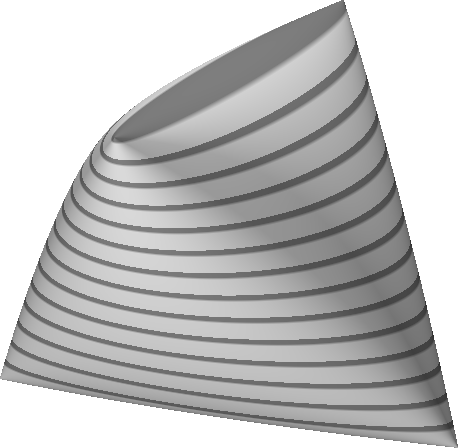
\includegraphics[width=150pt]{spectrahedron}} at (0pt,0pt);
	\node[align=left] at (7,0) {\(
		\begin{pmatrix} 1 & x_1 & x_2 \\ x_1 & 1 & x_3 \\ x_2 & x_3 & 1
		\end{pmatrix} \ \text{psd}
		\)
	};
	\end{tikzpicture}
\end{center}

The first thing we wish to do is discussing duality for SDP. We would like to use the results from the previous sections. While in the previous sections we worked with the duality with respect to the standard scalar product in $\R^n$, it is clear that the duality could have been introduced with respect to any scalar product and the results would still be the same. So, we can introduce the dual cone $(\cS_+^k)^\ast$ in the space $\cS^k$ just by the same formula that we used to introduce dual cones in $\R^n$.

It turns out that $\cS_+^k$ is self-dual.

\begin{exercise}
	For every $k \in \N$ one has $(\cS_+^k)^\ast = \cS_+^k$ (the cone $\cS_+^k$ is self-dual). 
\end{exercise}
\begin{solution} 
	For $A \in \cS^k$ the equality says that the condition $A \in \cS_+^k$ is equivalent to $\sprod{A}{B} \ge 0 \ \forall B \in \cS_+^k$. We check this equivalence.
	
	If $A \in \cS_+^k$, then  $\sprod{A x}{x} \ge 0$ holds for all $x$. The latter can be turned into the form $\sprod{A}{x x^\top} \ge 0$. Note that $x x^\top$ is a symmetric (psd) matrix of rank $1$ (for $x \ne 0$). The cone $\cS^k_+$ is the conic hull of all such matrices (see Exercise~\ref{sdp:sum:rank:1}). So, we get $\sprod{A}{B} \ge 0$ for all $B \in \cS_+^k$. Conversely: if $\sprod{A}{B} \ge 0$ holds for every $B \in \cS_+^k$, then choosing $B = x x^\top$, we get $\sprod{A}{x x^\top} \ge 0$ for all $x \in \R^n$. This gives $\sprod{A x}{x } \ge 0$ for all $x$ and shows $A \in \cS_+^k$. 
\end{solution}

\begin{exercise}
	Formulate the problem of computing the largest eigenvalue of a symmetric matrix as an SDP. 
\end{exercise}
\begin{solution}
	For $A \in \cS^k$ consider the matrix $t I - A$. It is easy to see that $\lambda$ is an eigenvalue of $A$ if and only if $t-\lambda$ is an eigenvalue of $t I - A$. A matrix $A \in \cS^k$ is PSD if and only if all its eigenvalues are non-negative. So, we arrive at the SDP
\begin{align*}
	\min \setcond{t \in \R}{ t I - A \in \cS_+^k}
\end{align*}
with one decision variable $t \in \R$.
This is an SDP in one unknown $t \in \R$. 
In the same way, we can see that computation of the spectral norm of a symmetric matrix is again an SDP (in one unknown).
\end{solution}

\begin{remark}
	Many researches are very excited about SDP. Why? It has turned out that a large number of problems can be formulated (exactly or approximately) as an SDP. In particular, we have seen that polynomial problems can be formulated approximately as SDPs. Apart from that, SDPs arise in control theory, combinatorial optimization, statistics, probability etc. Yet another reason for excitement is that SDP leads to interesting mathematical problems involving algebra, convexity and algorithms. 
\end{remark}

\subsection{Duality for SDP}

Using the previous section and conic duality, we can derive duality for SDPs. For duality in the space $\R^n$ we used the standard scalar product in $\R^n$, and the matrix $A$ (of the left hand side of the underlying system of constraints) in the primal problem has been turned to the transposed matrix $A^\top$ in the dual problem. Now, we work in $\cS^k$, which is a different Euclidean space, and so instead of using $A^\top$ we need to use an abstract analogue of it. The abstract transpose is called the adjoint operator. Actually, the adjoint operator is just another way of writing transpose (it's not more general in its essence, it's just a more general way of writing things down, that does not rely too much on the components). Let me shortly recall how this works (this material is typically presented in linear algebra). We've got two finite-dimensional Euclidean spaces $V$ and $W$ over $\R$. The spaces have scalar products  $\sprod{\dotvar}{\dotvar}_V$ and $\sprod{\dotvar}{\dotvar}_W$ (frequently, one would just omit the subscript, as it is usually clear which of the scalar products is meant). 

Consider a linear map $A : V \to W$ and a vector $b \in W$. With this data we can define an `abstract' linear system $A(x) = b$ in the unknown $x \in V$. An analogue of transpose matrix is the so-called \emph{adjoint operator} or \emph{adjoint map} $A^\ast : W \to V$, defined as the unique linear map satisfying $\sprod{A(x)}{y}_W = \sprod{x}{A^\ast(y)}_V$. 

In this abstract setting the dual pair of conic programs looks as follows

\[
	\inf \setcond{ \sprod{c}{x}}{ x \in K, \ A (x) - b \in L}
\]
and
\[
	\sup \setcond{ \sprod{y}{b}}{y \in L^\ast, \ c - A^\ast (y) \in K^\ast}
\]
where $K$ is a closed convex cone in $V$ and $L$ a closed convex cone in $W$. 



\newcommand{\cA}{\mathcal{A}}
We just need to specify what we get in the case of SDPs in the above formulas. For example, let's determine the dual of the SDP in the form
\[
	\inf \setcond{ \sprod{c}{x}}{ x_1 A_1 + \ldots + x_n A_n - B \in \cS_+^k}
\]

We can write it as 
\[
	\inf \setcond{ \sprod{c}{x}}{x \in \R^n, A(x) - B \in \cS_+^k}
\]
where $A : \R^n \to \cS^k$ is the linear map $A(x) = A_1 x_1 + \cdots + A_n x_n$. To get the dual we need to determine $A^\ast : \cS^k \to \R^n$. Just use the equality that defines the adjoint map:
\[
	\sprod{A(x)}{Y} = \sprod{x}{A^\ast(Y)} \qquad \forall x \in \R^n \ \forall Y \in \cS^k.
\]
This can be spelled out as
\[
	\sprod{A_1 x_1 + \ldots + A_n x_n}{Y} = \sprod{(x_1,\ldots,x_n)}{A^\ast(Y)} \qquad \forall x_1,\ldots,x_n \in \R \ \forall Y \in \cS^k.
\]
Comparing coefficients for $x_1,\ldots,x_n$ gives the formula 
\[
	A^\ast(Y) = ( \sprod{A_1}{Y},\ldots, \sprod{A_n}{Y})
\]
for the adjoint map.

Consequently, our dual problem is 
\[
	\sup \setcond{ \sprod{B}{Y}}{Y \in \cS_+^k, \ c_i = \sprod{A_i}{Y} \ \forall i \in [n]}
\]

\begin{remark}
	If you know the mnemonic rules to get a dual LP, you see that these rules carry over to the case of SDP in some very natural way. The mnemonic rule is about what corresponds to what in the primal-dual pair:
	\begin{itemize}
		\item variables $\leftrightarrow$ constraints
		\item unconstrained variables$\leftrightarrow$ equality constraints
		\item non-negative variables $\leftrightarrow$ inequality constraints;
		\item right hand sides $\leftrightarrow$ coefficients of the objective functions. 
	\end{itemize}
	We see that the rule remains valid for SDP.
	Our primal problem had $x_1,\ldots,x_n$ unconstrained real variables and one SDP constraint. The sdp constraint generates a psd-constrained variable $Y$ in the dual. The $n$ variables $x_1,\ldots,x_n$ generate the $n$ equality constraints in the dual. Note that our primal/dual pair of SDP illustrates the following: 
	\begin{itemize}
		\item real variables $\leftrightarrow$ LP constraints ($=$ linear (in)equalities)
		\item matrix variables $\leftrightarrow$ SDP constraints ($=$ LMIs).
	\end{itemize}
\end{remark}

\subsection{SDP duality applied to polynomial optimization}

Let's now apply the SDP duality to the SDP problem we derived in Section~\ref{SOS:and:sdp}. Let me remind what we did. We wanted to solve the global POP 
\begin{equation}
	\label{global:pop}
	\inf \setcond{f(x)}{ x \in \R^n },
\end{equation}
where $f(X)= \sum_{\gamma \in E^n_{2d}} c_\gamma X^\gamma \in \R[X]=\R[X_1,\ldots,X_n]$. We introduced the formal dual problem $\sup \setcond{y}{f - y \ge 0 \ \text{on} \  \R^n}$ (the problem to find the lower bounds) and then replaced this problem by the simpler problem
\[
	\sup \setcond{y \in \R}{ f - y \text{ is SOS}}, 
\]
which turned out to be the SDP
\[
	\sup \setcond{y \in \R}{ y + m(X)^\top Z m(X) = f(X), \ Z \ \text{psd}} ,
\]
where $m(X)= (X^\alpha)_{\alpha \in E^n_d}$ is the vector of monomials of degree at most $d$.
Thus, the above problem is a problem with decision variables $y$ and $Z$. To dualize the problem, we write the equality constraint $y + m(X)^\top Z m(X) = f(X)$ in coordinate form. Let $Z=(z_{\alpha,\beta})_{\alpha,\beta \in E^n_d}$. Then the equality $y + m(X)^\top Z m(X)= f(X)$ is 
\[
	y + \sum_{\alpha,\beta \in E^n_d} z_{\alpha,\beta} X^{\alpha+\beta} = \sum_{\gamma \in E^n_{2d}} c_\gamma X^\gamma.
\]
Comparing coefficients we get
\[
	y + z_{0,0} = c_0
\] 
and 
\begin{align*}
	\sum_{\alpha,\beta \in E^n_d : \ \alpha + \beta =\gamma} z_{\alpha,\beta} &=  c_\gamma & & \forall \gamma \in E^n_{2 d} \setminus \{0\}.
\end{align*}
%
The latter can be written as the equations
\begin{align*}
	y + \sprod{A_0}{Z}  = c_0
\end{align*}
and
\begin{align*}
	\sprod{A_\gamma}{Z} &= c_\gamma & &\forall \gamma \in E^n_{2d} \setminus \{0\},
\end{align*}
where
\begin{align*}
	A_\gamma &:= (\delta_{\alpha+\beta,\gamma})_{\alpha,\beta \in E^n_d} & & \forall \gamma \in E^n_{2d}
\end{align*}
are symmetric matrices (we use the Kronecker delta notation: $\delta_{s,t}=1$ if $s=t$ and $\delta_{s,t}=0$ otherwise).
Thus, our problem can now be written as 
%
\begin{equation}
	\label{global:sos:rel:with:equalities}
	\sup \setcond{y \in \R}{ Z \ \text{psd}, \ y+ \sprod{Z}{A_0} = c_0, \ \sprod{A_\gamma}{Z} = c_\gamma \ \text{for \ all} \ \gamma \in E^n_{2d} \setminus \{0\}}.
\end{equation}
%
Problem \eqref{global:sos:rel:with:equalities} can be dualized according to the principles we've discussed in previous sections.  The psd matrix variable $Z$ yields a psd constraint. The real variable $y$ yields a linear equation. Each linear equality constraint for $\gamma \in E_{2d}^n$ yields a real variable, which we denote by $v_\gamma$.

The dual is the following problem

\[
	\inf \setcond{ \sum_{\gamma \in E^n_{2d} } v_\gamma c_\gamma }{v_\gamma \in \R \ \forall \gamma \in E^n_{2d}, \ \sum_{\gamma \in E^n_{2d}} v_\gamma A_\gamma \ \text{psd}, \ v_0 = 1}.
\]
%
Taking into account how $A_\gamma$ were defined we see that 
\[
	\sum_{\gamma \in E^n_{2d}} v_\gamma A_\gamma = \Biggl( \sum_{\gamma \in E^n_{2d}} v_\gamma \delta_{\alpha + \beta,\gamma} \Biggr)_{\alpha, \beta \in E^n_d} = \Bigl( v_{\alpha+ \beta} \Bigr)_{\alpha, \beta \in E^n_d}.
\]
%
Hence, the dual SDP gets the form
\begin{equation}
	\label{global:sos:rel:with:equalities:simplified}
	\inf \setcond{ \sum_{\gamma \in E^n_{2d}} v_\gamma c_\gamma }{v_\gamma \in \R \ \forall \gamma, \ \Big(v_{\alpha+\beta}\Big)_{\alpha, \beta \in E^n_d} \ \text{psd}, \ v_0 = 1}.
\end{equation}
%
%
\begin{remark}
The problem \eqref{global:sos:rel:with:equalities} was established to derive lower bounds on \eqref{global:pop}, but \eqref{global:sos:rel:with:equalities} does not directly suggest any choice of $x \in \R^n$ that may be good. It turns out that an $x$ can be chosen from the dual problem. It is known that, under certain assumptions, $x=(x_1,\ldots,x_n)$ with 
\begin{align*}
 x_1 & := v_{(1,0,\ldots,0)}, & x_2 & := v_{(0,1,0\ldots,0)}, & & \ldots & x_n & := v_{(0,\ldots,0,1)}
\end{align*}
is a good choice (see works of Marshall, Schweighofer, Lasserre, Laurent et al.). 
\end{remark}
%
\blue{
\begin{example}
Let $f = X^2 - 2 X Y + 4 Y^2 - X - 2 Y + 3$.
The minimum of $f$ over~$\R^2$ equals~$2$ and is attained at the point $(1,\frac12)$.
The linear objective in the problem~\eqref{global:sos:rel:with:equalities:simplified} is given by
\[
3 - v_{10} - 2 v_{11} - 2 v_{01} + v_{20} + v_{02}
\]
and we minimize over all psd matrices of the form $V = (v_{\alpha+\beta})_{\alpha,\beta \in \{00,10,01\}}$ with $v_{00} = 1$.
The minimum is attained by
\[
V =
\left(
\begin{matrix}
1 & 1 & \frac12 \\
1 & 1 & \frac12 \\
\frac12 & \frac12 & \frac14
\end{matrix}
\right)
\]
with objective value~$2$ and $x_1 = v_{10} = 1$ and $x_2 = v_{01} = \frac12$.
\end{example}
}

\subsection{Truncated moment problem}

There is another way to arrive at the dual problem we've seen in the last section. 

We show how the approach works for the unconstrained POP only, with the constrained case being similar.
Consider

\begin{equation}
	\label{our:inf:problem}
	\inf \setcond{f(x) }{x \in \R^n}\,,
\end{equation}
with $f \in \R[X]=\R[X_1,\ldots,X_n]$. Let $c = (c_\alpha)_{\alpha \in E_{2d}^n}$ be the vector of coefficients of~$f$ and $m(X) = (X^\alpha)_{\alpha \in E_{2d}^n}$ the vector of all respective monomials. Then the problem can be written as 
\begin{equation}
	\inf \setcond{ \sprod{c}{m(x)} }{x \in \R^n}.
\end{equation}
This can be viewed as linear optimization over the set $m(\R^n):=\setcond{m(x)}{x \in \R^n}$. Thus, the problem is equivalent to
\begin{equation}
	\inf \setcond{\sprod{c}{v}}{v \in m(\R^n)}.
\end{equation}
If we enlarge $m(\R^n)$ to $\conv(m(\R^n))$ or even to $\cl(\conv(m(\R^n)))$, the problem remains the same. This way we arrive at 
\begin{equation}
	\label{lin:probl:on:M}
	\inf \setcond{\sprod{c}{v}}{ v \in M_{n,2d}}\,, \quad \blue{\textrm{ where } \quad M_{n,2d} := \cl(\conv(m(\R^n)))} \,.
\end{equation}
In general, $M_{n,2d}$ is hard to describe, but at least we can relax it to a set that we can describe with an SDP. By Carath\'{e}odory's theorem, every element of $v \in \conv(m(\R^n))$ is the convex combination of at most $\dim(m(\R^n))+1$ points of $m(\R^n)$. This convex combination can be written as the integral
\[
	v = v^\mu:= \int m(x) \mu( d x) \,,
\]
with respect to a finitely supported probability measure $\mu$ on $\R^n$. Using the definition of Lebesgue integrability, one can show that if $\mu$ is any probability measure on $\R^n$, for which the above integral exists, the respective vector $v^\mu$ belongs to $M_{n,2d}=\cl(\blue{\conv(m(\R^n))})$; see \cite[Definitions~11.21, 11.22]{Rudin}. Note that $v^\mu$ is called the \emph{vector of moments} of $\mu$ of order at most $2d$. The problem of characterizing whether a given collection of numbers associated to the multi-indices $\alpha \in \Z_+^n$ is a collection of moments of a probability measure supported in a given set $S$ is a well-known problem in probability theory and it is known as the \emph{problem of moments}. So, what special properties does the vector $v^\mu$ have? Consider an arbitrary vector $y=(y_\alpha)_{\alpha \in E_d^n} \in \R^{\binom{n+d}{n}}$. Of course $v^\mu_0=1$, since $\mu$ is a probability measure. Furthermore, for the matrix $A(v^\mu) = (v^\mu_{\alpha+\beta})_{\alpha,\beta \in E_d^n}$ one has
\begin{align*}
	y^\top A(v^\mu) y \ = \int x^{\alpha + \beta} y_\alpha y_\beta \mu(d x)
 = \left( \int x^\alpha y_\alpha \mu(d x)\right)^2 
 \ge 0.
\end{align*}
That is, $A(v^\mu)$ is PSD and \eqref{lin:probl:on:M} can be relaxed to 
\begin{equation}
	\label{moment:relaxation}
	\inf \setcond{\sprod{c}{v}}{v_0=1, \ A(v) \ \text{psd}}.
\end{equation}
This is an SDP, because the condition that $A(v)$ is PSD is a linear matrix inequality. The matrix $A(v)$ is called a \emph{localizing matrix}. 
This is just the same problem we obtained in the previous section through dualization of the SOS relaxation. 

In the constrained case, the arguments are quite similar and one also gets similar inequalities. Just to give one example. Let $\mu$ be a measure supported on the set $\{g \ge 0\}$, where $g = \sum_\alpha g_\alpha X^\alpha$ is a polynomial, and assume that $v^\mu$ is well-defined. Then, for every $y=(y_\beta)_\beta$ one has
\[
	\int g(x) \left( \sum_\beta x^\beta \right)^2 \mu( d x) \ge 0 \,,
\] 
which again turns out to be a condition $y^\top A_g(v^\mu) y$ for some matrix $A_g$. Thus we arrive at linear matrix inequalities (of a bit more general form). 

The above considerations show that the problem of moments and the positivstellens{\"a}tze and nichtnegativstellensätze are closely linked. By characterizing non-negativity of a polynomial on $\R, [0,+\infty),[0,1]$ in terms of SOS, we arrive at a characterization of sequences of moments of probability measures supported by the respective sets. All these are classical results in measure theory and probability theory.
 

\subsection{Peculiarities of SDP}

In contrast to LP, there are difficulties in solving SDP in exact arithmetics, as the following two exercises indicate. 

\begin{exercise}
	Show that even if the input data of an SDP (coefficients of vectors and matrices) is rational, the optimal solution need not be rational. 
\end{exercise}
\begin{solution}
	One can formulate the problem $\min \setcond{y}{y \ge x^2, \ y \ge 1 -x}$ as an sdp. The minimum is attained for \blue{any $x \in \R$} with $x^2 = 1 -x$, which is not a rational number.
\end{solution}

\begin{exercise}
	Even if the input data and the optimal solution of an SDP are rational, the encoding size of the output can be huge (the encoding size is the number of one needs to write down the solution, if one encodes rational values through numerator and denominator and the numerators and denominators are encoded in binary system). By huge, we mean exponential in the size of the input. 
\end{exercise}
\begin{solution}
	Consider the constraints $x_j \ge x_{j-1}^2$ for $j > 1$, for variables $x_1,\ldots,x_n$ with the constraint $x_1 \ge \frac{1}{2}$. Minimizing $x_n$ under these constraints gives the optimal solution $(x_1,\ldots,x_n) = (\frac{1}{2}, \frac{1}{2^2},\ldots,\frac{1}{2^{2^n}})$. So for encoding $x_n$ (in the standard form) one would need exponentially many bits. 
\end{solution}

\begin{exercise}
	Show that, in contrast to LP, for SDP the finite optimum value (infimum/supremum) is not necessarily attained. 
\end{exercise}
\begin{solution}
	To get examples confirming this, it helps to know that the second-order-cone programming is a special case of SDP (this is the topic of Section~\ref{soc:programming} below). So, also optimizing over conic sections is a special case of SDP. Two-dimensional conic sections are parabola or hyperbola or two lines. And the hyperbola is what we can use. If say, $x_1, x_2 \ge 0$ and $x_1 x_2 \ge 1$, then we cannot attain $x_1=0$ but can come arbitrarily close to $0$. Modeling $x_1 x_2 \ge 1$ as an sdp constraint is not a problem. 
\end{solution}


\begin{exercise}
	In degenerate situations, one can have a positive duality gap. Consider for example the problem
	\[
		\inf \setcond{x}{ \begin{pmatrix} 0 & x \\ x & y \end{pmatrix} \ \text{psd}, x  \ge -1 }
	\]
	What is the optimal value? What is the optimal value of the dual?
\end{exercise}
\begin{solution}
	I think, the example goes back to Lov\'asz. 
	The optimal value of this problem is $0$. 
Let's establish the dual. The psd constraint produces a matrix variable $Z \in \cS_2^+$ and the linear constraint the scalar variable $u \ge 0$. The objective function is $-u$. Since $x, y$ are unconstrained variables, there will be two equality constraints on the entries of $Z$. 
\[
\max \setcond{-u}{u \in \R_+, \ Z \in \cS_2^+,  \sprod{Z}{\begin{pmatrix} 0 & 1 \\ 1 & 0 \end{pmatrix} } + u =  1, \sprod{Z}{\begin{pmatrix} 0 & 0 \\ 0 & 1 \end{pmatrix} } =  0}
\]
Written in a bit simpler notation 
\[
\max \setcond{-u}{u \ge 0, \begin{pmatrix} z_{11} & z_{12} \\ z_{12} & 0 \end{pmatrix} \ \text{sdp}, \ 2 z_{12} + u = 1}
\]
The sdp constraint gives $z_{12} = 0$, so that for every feasible solution we get $u=1$. Thus, the optimal solution is $-1$, which means that we have a positive finite duality gap. 
\end{solution}


\subsection{Detour: Second-order cone programming}

\label{soc:programming}

This subsection is not necessary for discussing polynomial optimization. It can be read if you want to learn more about the connection of semidefinite optimization to other classes of optimization problems. 

	\emph{Second-order cone programming (second order cone problem)} (SOCP for short) is more general than LP and less general than SDP. SOCP is the conic programming with respect to the second-order cones 
	\[
		\SOC_{n}:=\setcond{(x,y)}{x \in \R^n, y \ge \|x \|} \subseteq \R^{n+1}.
	\]
	In particular, $\SOC_0=\R_+$. Thus, LP is indeed a special case.
	
	SOCPs can be written in the following form 
	\[
		\inf \setcond{ \sprod{c}{x} }{ \sprod{a_i}{x} + \beta_i \ge \| A_i x + b_i \| \ \forall i \in [t]},
	\]
	where $\beta_1,\ldots,\beta_t$ are scalars, $c,a_1,\ldots,a_t,b_1,\ldots,b_t$ are vectors  $A_1,\ldots,A_t$ are matrices. Also, from this formulation we see that LP is just the case $A_i=0$ and $b_i=0$.  
	
	\begin{exercise}
	 Show that SOCP is a special case of SDP. It suffices to write  $y \ge  \| x \|$ as an LMI. 
	\end{exercise}
	\begin{solution}
	 We write  $y \ge \| x \|$ as $y \ge 0$ and $y^2 \ge x^\top x$.  This condition can be written as the LMI $A(x,y) \in \cS_+^{n+1}$ with
	\[
	A(x,y) = \begin{pmatrix} 
	y I & x
	\\ x^\top & y
	\end{pmatrix}.
	\]
	Let's take a look at the condition $A(x,y) \in \cS_+^{n+1}$. It turns out to be useful to consider 
	\[
		\det A(x,1) = \det \begin{pmatrix} 
		 I & x
		\\ x^\top & 1
		\end{pmatrix} .
	\]
	The matrix $A(x,1)$ can be brought to a lower triangular form by subtracting a linear combination of the $n$ first columns from the last one. The lower triangular matrix will have $1,\ldots,1, 1- \| x \|^2$ on the diagonal. Thus $\det A(x,1) = 1 - \| x \|^2$. Viewing the determinant as an element of $\R[x,y] = \R[x_1,\ldots,x_n,y]$, we compute
	\begin{align*}
		\det A(x,y) = \det (y A(x/y,1)) = y^{n+1} ( 1 - \frac{1}{y^2} \| x\|^2) = y^{n-1}( y^2  - \|x\|^2). 
	\end{align*}
	
	It follows that $\det A(x,y-\lambda) = (y-\lambda)^{n-1} ((y-\lambda)^2 - \|x\|^2)$. This shows that the eigenvalues of $A(x,y)$ are $\lambda = y$ and $\lambda = y \pm \| x \|$. Consequently, $A(x,y)$ is psd if and only if $y \ge \| x \| $ is fulfilled.
	\end{solution}
	
	\begin{remark}
		Of course, when it comes to solving SOCP it is better to use solvers tailored to SOCP rather than reducing SOCP to SDP. Nevertheless, the above reduction shows what kind of problem classes can be found in SDP (which is important to understand). 
	\end{remark}
	
\subsection{Detour: Linear stochastic optimization}

This subsection, too, is optional. It sort of continues the discussion started in the previous subsection. 

Stochastic versions of non-stochastic optimization problems arise by allowing random coefficients (in the constraints and/or the objective function). It may not be immediately clear what it means to solve a stochastic problem. If constraints are stochastic, one may want to satisfy each of them with a certain probability. The following exercise show that stochastic linear programming can be connected to (non-stochastic) SOCP.

\newcommand{\oa}{\overline{a}}

\begin{exercise}
	 We consider a linear program with the non-stochastic objective $\sprod{c}{x}$, non-stochastic rand hand sides and stochastic left hand sides. The problem is 
	\[
		\inf \setcond{ \sprod{c}{x} }{ \operatorname{Prob} [ \sprod{a_i}{x} \le b_i ] \ge p \ \forall i \in [m]}
	\]
	with independent Gaussian vectors $a_i \sim N(\oa_i,C_i)$ having expectations $\bar{a_i} \in \R^n$ and covariance matrices $C_i \in \cS_+^n$. The value $p \in (0,1)$ is a certain threshold (tolerance).
	Show that the above problem can be formulated as SOCP. 
\end{exercise}
\begin{solution}
Let's spell out one such constraint (we omit indices to have a simpler notation)
\begin{equation}
\label{eq:stoch:nebenbedingung}
\operatorname{Prob}[ \sprod{a}{x} \le b ] \ge p
\end{equation}
with $a \in N(\oa,C)$, $\oa \in \R^n$ and $C \in \cS_+^n$. We can represent $a$ as $a = C^{1/2} \xi + \bar{a}$ with $\xi = (\xi_1,\ldots,\xi_n)$ and  iid $\xi_1,\ldots,\xi_n \in N(0,1)$. The condition $\sprod{a}{x}  \le b$ can be formulated as $\sprod{\xi}{C^{1/2} x} \le b - \sprod{\oa}{x}$. If $C^{1/2} x = 0$ the condition is deterministic, it is just $b - \sprod{\oa}{x} \ge 0$. Otherwise, we rewrite it as $\eta:= \sprod{\xi}{ \frac{C^{1/2} x}{\| C^{1/2} x \|}} \le \frac{b-\sprod{\oa}{x}}{\| C^{1/2} x \|}$. Clearly, $\eta \sim N(0,1)$. Thus, the condition can be written as
\[
\frac{b - \sprod{\oa}{x}}{\| C^{1/2} x \|} \ge \Phi^{-1} (p)
\]
using the distribution function $\Phi : \R \to [0,1]$ of $N(0,1)$. We have thus shown that \eqref{eq:stoch:nebenbedingung} is a conic constraint
\[
b - \sprod{\oa}{x} \ge \Phi^{-1}(p) \| C^{1/2} x \|,
\]
In the case $C = 0$, we just get a linear constraint. 
\end{solution}








\clearpage
\section{Interior-point methods for linear and semidefinite optimization} 

In principle, one could start directly with the discussion of interior-point methods for SDP, to shorten the presentation. However, it is easier to understand the technicalities of the SDP case, if one got the idea of interior-point methods for LP first. So, we first describe general ideas, then discuss LP and then go over to SDP.

\subsection{Ways to solve constrained convex problems: a very short synopsis}

We are talking about sufficiently smooth problems here. % Methods to find locally optimal solutions for constrained and unconstrained optimization were discussed by Sebastian Sager. 
Unconstrained problems can be solved by first and second order methods (gradient descent, Newton and the many generalizations and ramifications thereof). To solve constrained problems, one basic approach is to approximate the original problem by an unconstrained problem by `deforming' the objective functions. So, we replace the original problem by a so-called auxiliary problem (with an auxiliary objective function), which is unconstrained (or as good as unconstrained).  One can distinguish between penalty and barrier methods. In barrier methods we end up with optimizing a function over an open set (which is, more or less, unconstrained optimization). In penalty methods, the auxiliary function is defined on the whole space and the optimal solution for the auxiliary problem may not be feasible (but is hopefully almost feasible) for the original problem.

Yet, another method is the ellipsoid method. In principle, it can be applied for LP, SDP and other problems and it can be used to show solvability in polynomial time, but by now it has only been of theoretical importance.

For solving SDP we are free to choose any of the methods listed above; however, so far the interior-point methods have been the most successful ones. To develop an interior-point method, we need to decide which barrier we could use and then to figure out how to compute the derivatives of the modified objective function. 

\subsection{Central path for LP with constraints \texorpdfstring{$Ax \le b$}{Ax <= b}}

Consider the system $A x \le b$ which we can write as $\sprod{a_i}{x} \le b_i$, so $a_1,\ldots,a_m$ are the rows of $A$. We assume that the polyhedron $P$ defined by $A x \le b$ has non-empty interior. We assume that none of the inequalities are trivial ones having the form $\sprod{0}{x} \le 0$. In this case the interior of $P$ is described by $A x < b$. We introduce the objective $f(x) = \sprod{c}{x}$. Our problem is $\inf \setcond{f(x)}{x \in P}$. For every $\mu \ge 0$ consider the auxiliary objective function 
\[
	f_\mu(x) = \sprod{c}{x} - \mu \sum_{i=1}^m \ln(b_i- \sprod{a_i}{x})
\]
The sum of the logarithms is called a barrier function. For each given $\mu> 0$, we get the auxiliary problem $\min \setcond{f_\mu(x)}{x \in \intr(P)}$. 

\begin{exercise}
	Show that, if the above assumptions on $P$ are fulfilled, and $P$ is bounded, then $f_\mu$ is strictly convex on $\intr(P)$. Show that $f_\mu$ attains its infimum on $\intr(P)$. 
\end{exercise}

Thus, if $P$ is bounded, the auxiliary problem has a unique optimal solution $x^\ast(\mu)$. The map $\mu \mapsto x^\ast(\mu)$ is a parameterization of a curve (the so-called \emph{central path}). 

The idea of central path methods is to start with $x^\ast(\mu)$ for some $\mu>0$ and then decrease $\mu$ until a desired accuracy is reached. If $\mu_2 \ge \mu_1$ and $x^\ast(\mu_2)$ is given we can use $x^\ast(\mu_2)$ as an approximation for $x^\ast(\mu_1)$, so that one can invoke various kinds of iterative methods (most notably Newton and damped Newton) that would start with $x^\ast(\mu_2)$ to determine $x^\ast(\mu_1)$. In this way, we can gradually decrease $\mu$ reaching arbitrarily small values and making our auxiliary problem arbitrarily close to the original one.

\subsection{Central path for LP with constraints \texorpdfstring{$Ax=b, x \ge 0$}{Ax = b, x >= 0}}

Here we consider the problem in the form 
\[
	\min \setcond{\sprod{c}{x}}{A x = b, x \ge 0}.
\]
where $A \in \R^{m \times n}$, $b \in \R^m$ and $x=(x_1,\ldots,x_n)$ is the vector of decision variables.
We assume that there exists $x > 0$ with $A x =b$. In that case we can introduce the auxiliary  problem $\inf \setcond{f_\mu(x)}{A x= b, x > 0}$ with the auxiliary objective 
\[
	f_\mu(x) = \sprod{c}{x} - \mu \sum_{j=1}^n \ln x_j
\]
where $\mu>0$ is a parameter. For the function $f_\mu$ defined on $\setcond{x}{A x =b, x >0}$ one can establish analogous properties as for the function from the previous section (it is strictly convex and the optimum is attained, when $\setcond{x}{A x=b,x \ge 0}$ is bounded). 

Since $f_\mu$ is convex, a necessary and a sufficient condition for $x >0$ to be optimal for $f_\mu(x)$ is that $Ax =b$ is fulfilled and $\nabla f_\mu(x)$ is orthogonal to the space $A x =b$. Since $\setcond{x}{A x =b}$ coincides with $\ker(A)$ up to translations, we get the condition $\nabla f_\mu(x) \in \ker(A)^\perp$. Since $\ker(A)^\perp = \im(A^\top)$, the condition can be rewritten as $\nabla f_\mu(x) \in \im(A^\top)$. The latter means that $\nabla f_\mu(x)$ is in the linear hull of the columns of $A$. The condition $\nabla f_\mu(x) \in \im(A^\top)$ is exactly the KKT condition, phrased in geometric terms. Noticing that $\nabla f_\mu(x) = c+ \mu (1/x_1,\ldots,1/x_n)$, we can now formulate the KKT conditions as
\begin{align*}
	A x & = b,
	\\ 	c+ \mu (1/x_1,\ldots,1/x_n) & = A^\top y
\end{align*}
where $y \in \R^m$. Introducing the vector $s= \mu (1/x_1,\ldots,1/x_n)$, we can rewrite the latter conditions as 

\begin{align}
	A x & = b, \label{primal:eq}
	\\ A^\top y - s & = c \label{dual:eq}
	\\ (s_1 x_1,\ldots,s_n x_n) & = \mu (1,\ldots,1) \label{mu:slack}
	\\ x, s & > 0. \label{strict:pos}
\end{align}

All the equations are linear apart from the equations $s_i x_i = \mu$. 


	For solving the system \eqref{primal:eq}--\eqref{strict:pos} we can use the Newton method. If we have an approximate solution $x, y, s$, which satisfies $A x = b$ and $A^\top y -s  =c$ exactly and satisfies the conditions $x_i s_i = \mu$ approximately, we can try to determine a better solution in the form $x + \Delta x, y + \Delta y, s + \Delta s$. For $\Delta x, \Delta y$ and $\Delta s$, we obtain the conditions $A \Delta x = 0$, $A^\top \Delta y - \Delta s = 0$. By linearizing the condition $(s_i + \Delta s_i) (x_i + \Delta x_i)  = \mu$ removing the quadratic term $\Delta s_i \Delta x_i$, we arrive at $s_i \Delta x_i + \Delta s_i x_i = \mu - s_i x_i$. The variables $\Delta s_i$ can be eliminated, as we can express them via $\Delta y$. In this way we end up with a linear system of equalities in the unknowns $\Delta x, \Delta y$. The size of the system is $m+n$. If $A$ has full row rank (which we can assume wlog), then the latter system has a unique solution). We would have to take care that the update produces a solution which is still positive (so, we are on the safe side if we use damped Newton). 

	Let's estimate how well the auxiliary problem approximates the original one. In view of the boundedness assumption LP duality gives us the equality
	\[
		\alpha := \min \setcond{ \sprod{c}{x} }{x \in \R^n, \ A x = b, x \ge 0} = \max \setcond{ \sprod{b}{y}}{ y \in \R^m, \ A^\top y \le c} \in \R.
	\]
	of the optimal values of the primal and the dual problem. 
	The dual problem can also be written using the slack vector $s \ge 0$ as $A^\top y + s = c, y \in \R^m s \in \R_+^n$. We can thus see now that this version of the central path method constructs a primal/dual pair of solutions. It turns out, these solutions get nearly optimal as $\mu \to 0$. 
	
	Indeed, repeating the derivation of the weak duality, we get the estimates
	\[
		\alpha \ge \sprod{b}{y} = \sprod{A x}{y}= \sprod{x}{A^\top y} = \sprod{x}{c-s} = \sprod{x}{c} - \sprod{x}{s} = \sprod{x}{c} - n \mu \ge \alpha - n \mu.
	\]
	Hence 
	\[
		\alpha - n \mu \le \sprod{b}{y} \le \alpha 
	\]
	and 
	\[
		\alpha \le \sprod{c}{x} \le \alpha + n \mu.
	\]
	So, our solutions are optimal up to the additive tolerance $n \mu$. 

\subsection{\texorpdfstring{$\ln(\det(X))$}{ln(det(X))} is a good barrier for SDP}

A natural barrier we can employ for the SDP cone is $\ln(\det(X))$. Indeed, on the boundary of $\cS_+^k$ the determinant gets zero, while in the interior of $\cS_+^k$ the determinant is strictly positive. So, taking the logarithm, we create a function that goes to (minus) infinity on the boundary. This is exactly what we want. 

For the auxiliary problem to be convex, the respective barrier needs to be a convex (or concave) function. We'll verify that $\ln(\det(X))$ is concave in $X$. Furthermore, in order to be able to apply first and second order methods for solving the auxiliary problem, we need to determine the first and the second derivatives of $\ln(\det(X))$. Note that the gradient and the Hesse matrix in an abstract Euclidean space can be defined analogously to the concrete space $\R^n$. That is, $\nabla f(x^\ast)$ satisfies $f(x) = f(x^\ast) + \sprod{\nabla f(x^\ast)}{x-x^\ast} + o(\|x-x^\ast\|)$, where $o(x-x^\ast)$ is a function with $o(\|x-x^\ast\|) / \|x-x^\ast\| \to 0$ for $x \to x^\ast$ and the `Hesse-Matrix' $\nabla^2 f(x^\ast)$ is a self-adjoint operator satisfying $f(x) = f(x^\ast) + \sprod{\nabla f(x^\ast)}{x-x^\ast} + \frac{1}{2} \sprod{\nabla^2 f(x^\ast) (x-x^\ast)}{x-x^\ast} + o(\|x-x^\ast\|^2)$. 


\begin{exercise}[Root of a psd matrix]
	\label{matrix:root}
	Show that for every $X \in \cS_+^k$, there exists a uniquely defined matrix $X^{1/2} \in \cS_+^k$ satisfying $(X^{1/2})^2 = X$. 
\end{exercise}
\begin{solution}
	We can write $\R^n = V_1 \oplus \ldots \oplus V_m$, where $V_1,\ldots,V_m$ are eigenspaces of $X$ to the $m$ pairwise distinct eigenvalues $\lambda_1,\ldots,\lambda_m \ge 0$. Thus, we can choose $X^{1/2}$ that sends $v \in V_i$ to $\lambda_i^{1/2} v$ on $V_i$. It remains to show uniqueness. Let $Y \in \cS_+^k$ satisfy $Y^2 = X$. We consider eigenspaces $W_1,\ldots,W_s$ of $Y$ to its eigenvalues $\mu_1,\ldots,\mu_s$. Because of $Y^2=X$ we see that $W_1,\ldots,W_s$ are eigenspaces of $X$ to the eigenvalues $\mu_1^2,\ldots,\mu_s^2$. So, we get $s=m$ and up to permutation of indices we must have $\mu_i^2 = \lambda_i$ for all $i \in [m]$.
\end{solution}

\begin{exercise}
	\label{interchange}
	For all $A, B \in \R^{n \times n}$ one has $\tr(AB)=\tr(BA)$. 
\end{exercise}
\begin{solution}
	Use the formula for the product of matrices and the formula for the trace (as the sum of diagonal entries) and see that the left and the right hand side are just the same. 
\end{solution}

\begin{proposition}[{see, for example, Renegar, \S 1.2}]
	The function $f : \intr(\cS_+^k) \to \R$ given by $f(X) := \ln (\det (X))$ is strictly concave and infinitely differentiable. Its gradient is 
	\[
		\nabla f(X) = X^{-1}
	\]
	and its `Hesse-Matrix' is the operator
	\[
		(\nabla^2 f(X)) (U) = X^{-1} U X^{-1}
	\]
	These two formulas can also be summarized as the second-order Taylor expansion 
	\[
		f(X+U) = f(X) + \sprod{X^{-1}}{U} + \frac{1}{2} \sprod{X^{-1} U X^{-1} }{U} + o(\|U\|^2), \qquad \text{as} \ U \to 0
	\]
	for every $X \in \intr(\cS_+^k)$. (The norm $\|U\|$ is the norm with respect to the scalar product that we fixed in $\cS^k$; it is the so-called Frobenius norm)
\end{proposition}
\begin{proof}
	Note that $\det(X)$ is a polynomial function with respect to the components of $X$ and it is strictly positive on $\intr(S^k)$. The function $\ln$ is infinitely differentiable on $\R_{>0}$. So, $f$ is infinitely differentiable. 
	
	\emph{Strict concavity of $f$}. It suffices to check the strict concavity on each line. This means that we check the strict concavity of $\phi(t) = \ln \det(X+ t U)$ for every $X \in \cS_+^k \setminus \{0\}$ and every $U \in \cS^k \setminus \{0\}$. We do this by showing that the second derivative is strictly negative
	
	\begin{align*}
		\phi(t) & = \ln ( \det(X^{1/2} X^{1/2} + t U) )
		\\ & =  \ln \bigl(\det(X^{1/2} (I + t X^{-1/2} U X^{-1/2}) X^{1/2}) \bigr)
		\\ & = \ln \bigl( \det(X^{1/2}) \det(I + t X^{-1/2} U X^{-1/2}) \det(X^{1/2}) \bigr)
		\\ & = \ln \bigl( \det(X) \det(I+ t X^{-1/2} U X^{-1/2}) \bigr)
	\end{align*}
	where $X^{-1/2} = (X^{1/2})^{-1}$. Let's use the notation  $\Tilde{U}:=X^{-1/2} U X^{-1/2}$. This gives
	\begin{align*}
		\phi(t) = \ln(\det(X)) + \ln \det(I+ t \Tilde{U}).
	\end{align*}
	It suffices to compute the derivative of $\ln \det(I + t \Tilde{U})$. $\Tilde{U}$ is symmetric, and we introduce its eigenvalues $\Tilde{\lambda}_i$ (taking into account the multiplicities). Then $1 + t \Tilde{\lambda}_i$ are the eigenvalues of $I + t \Tilde{U}$. Since $I + t \Tilde{U}$ (for $X + t U \in \intr(\cS_+^k)$) is positive definite, we have $1 + t \Tilde{\lambda}_i > 0$. Since the determinant of a symmetric matrix is a product of all the eigenvalues, we obtain 
	\[
		\phi'(t) = \sum_{i=1}^n \parti{}{t} \ln(1+ t \Tilde{\lambda}_i) = \sum_{i=1}^n \frac{\Tilde{\lambda}_i}{1 + t \Tilde{\lambda}_i}.
	\]
	and the second derivative is 
	\[
		\phi''(t) = - \sum_{i=1}^n \frac{ \Tilde{\lambda}_i^2}{ (1 + t \Tilde{\lambda}_i)^2}
	\]
	We have $\phi''(t) \le 0$. We cannot have $\phi''(t) = 0$, because this would imply $\Tilde{\lambda}_i = 0$ for all $i$. But then we'd have $\Tilde{U} = 0$ and by this $U = 0$.
	
	For computing the gradient of $f$ we can use the above computation for  $\phi'(t)$. We get
	\[
		\phi'(0)= \sum_{i=1}^n \Tilde{\lambda}_i = \tr(X^{-1/2} U X^{-1/2}) = \tr( X^{-1/2} X^{-1/2} U) = \tr(X^{-1} U) = \sprod{X^{-1}}{U}.
	\]
	So, we get the `directional' derivative
	\[
		\parti{f}{U}(X) = \sprod{X^{-1}}{U}
	\]
	which gives $\nabla f(X) = X^{-1}$. 
	
	For the derivation of the `Hesse-Matrix' we can use the above equation for $\phi''(t)$. We get
	\begin{align*}
		\phi''(0) = - \sum_{i=1}^n \Tilde{\lambda}_i^2 = \tr( \Tilde{U}^2) & = \tr(X^{-1/2} U X^{-1/2} X^{-1/2} U X^{-1/2} ) 	
		\\ & = \tr(X^{-1/2} U X^{-1} U X^{-1/2}) 
		\\ & = \tr(U X^{-1} U X^{-1} )  & & \text{(by Exercise~\ref{interchange})}
		\\ & = \sprod{U}{X^{-1} U X^{-1}}.
	\end{align*}
\end{proof}


\subsection{Interior-point methods for SDP}

I rely more or less on Chapter~6 of \cite{Gaertner:Matousek:2012}.

Let's consider the SDP

\[
	\inf \setcond{ \sprod{C}{X} }{X\in \cS_+^k, \ \sprod{A_i}{X}=b_i ~ \forall i \in [m]}.
\]

We assume that the problem is strictly feasible, that is, there exists $X \in \intr(\cS_+^k)$ with $\sprod{A_i}{X} = b_i$ for all $i \in [m]$. We introduce a parameter $\mu > 0$ and introduce the auxiliary problem
\[
	\inf \setcond{ \sprod{C}{X} - \mu \ln(\det(X)) }{X \in \intr(\cS_+^k), \ \sprod{A_i}{X} = b_i \ \forall i \in [m]}.
\]

Our auxiliary objective function $f_\mu(X)$ is strictly convex and the the infimum is actually a minimum, because $f_\mu(X) \to \infty$ when $X$ approaches the boundary of $\cS_+^k$. Due to the strict convexity, the minimum is unique. By KKT-condition, the gradient of $f_\mu$ is orthogonal to the affine space $\setcond{X \in \cS^k}{\sprod{A_i}{X}=b_i \ \forall i \in [m]}$. Thus, we can write the gradient of $f_\mu$ as a linear combination of the `normal vectors' $A_i$ of the hyperplanes $\sprod{A_i}{X}=b_i$. So, we arrive at the condition 

\[
	C - \mu X^{-1} = \sum_{i=1}^m y_i A_i
\]

We introduce the matrix $S = \mu X^{-1}$, for which the identity $S X = \mu I$ holds. Summarizing, we arrive at the system

\begin{align}
	X, S & \in \intr(\cS_+^k),  \ y_1,\ldots,y_m \in \R \label{eq:prim:dual:var} \\
	\sprod{A_i}{X} & = b_i \label{eq:lin:eq} \qquad \forall i \in [m]\\
		S + \sum_{i=1}^m y_i A_i & = C,  \label{eq:prim:dual:lin:eq}\\ 
	S X & = \mu I. \label{eq:mu:slackness}
\end{align}

As in the case of LP, one can see that $y_1,\ldots,y_m$ satisfying the above conditions is a feasible solution of the dual problem: 

\[
	\sup \setcond{y_1 b_1 + \cdots + y_m b_m}{ C - \sum_{i=1}^m y_i A_i \in \cS_+^k}.
\]

Note also that $S X  = \mu I$ is a kind of modified complementary slackness. 

Again, \eqref{eq:prim:dual:var}--\eqref{eq:mu:slackness} can be solved using iterative methods (say, damped Newton). Assume that we have $X,S,y_1,\ldots,y_m$ that satisfy all the above constraints exactly, except for the constraint $S X = \mu I$, which is only satisfied approximately.

For updating the current approximation $X,S,y_1,\ldots,y_m$ to a new $X+\Delta{X}, S + \Delta{S}, y_1 + \Delta{y_1},\ldots,y_m + \Delta{y_m}$, we plug in the new approximation and linearize the last constraint with respect to the $\Delta{S}$ and $\Delta{X}$:

\begin{align}
	\sprod{A_i}{\Delta X} & = 0, \qquad \forall i \in [m] \label{eq:for:delta:1}
	\\ \Delta{S} + \sum_{i=1}^m \Delta{y_i} A_i & = 0,\label{eq:for:delta:2}
	\\ \Delta{S} X + S \Delta{X} & = \mu I - S X \label{eq:for:delta:3}
\end{align}

That is the point, where the theory of interior-point methods for SDP starts. We've got a system of linear equations. Solving such equations is linear algebra, but the size is large and we want to solve the system approximately. 

Various approaches exist. One approach is to first give up the symmetry of $\Delta{X}$ and then do an update using  $(\Delta{X} + \Delta{X}^\top) /2$ rather than $\Delta{X}$. With this approach, from \eqref{eq:for:delta:3} we get 

\[
	\Delta{X} = \mu S^{-1} - X - S^{-1} \Delta{S} X.
\]
We plug in $\Delta{S}$ from \eqref{eq:for:delta:2} and get 
\[
	\Delta{X} = \mu S^{-1} - X + \sum_{j=1}^m \Delta{y}_j S^{-1} A_j X.
\]

Inserting this expression for $\Delta{X}$ into \eqref{eq:for:delta:1}, which can be written as \mbox{$\tr(A_i \Delta{X}) = 0$}, we arrive at the equation 

\[
	\sum_{j=1}^m \tr(A_i S^{-1} A_j X) \Delta{y}_j = \tr((X - \mu S^{-1}) A_i).
\]

This is a $m \times m$ linear system. It can be shown that, if $A_1,\ldots,A_m$ are linearly independent vectors of the space $\cS^k$, then the matrix of the system is symmetric positive definite (so that there exists a unique solution). The method of finding the non-symmetric $\Delta X$ and then symmetrizing works well in practice (though polynomial time bounds on the number of iterations are obtained using different, more involved methods, references can be found in \cite{Gaertner:Matousek:2012}). Regarding the complexity: Determination of $\Delta{X}$ can be viewed as solving $k$ linear equations of size $k \times k$. So, $O(k^4)$ operations. Solving the linear system for the $\Delta{y}_1,\ldots,\Delta{y}_m$ requires $O(m^3)$ operations. Note that $m$ can be as large as $O(k^2)$. Thus, we end up with $O(m^3) = O(k^6)$. When $m$ is not large, say $m=O(k)$, we still have $O(k^4)$ in one iteration of the Newton step. In the applications related to polynomial optimization, both $m$ and $k$ are big. So, one is forced to work with really huge matrices.

\clearpage
\bibliographystyle{amsalpha}
\bibliography{references}

%\appendix


%\input{Ablauf_WiSe_16_17.tex}



\end{document}
